\chapter{Methodology}

\section{Conceptual Framework}
\label{sec:conceptual}

\begin{figure}[H]
    \centering
    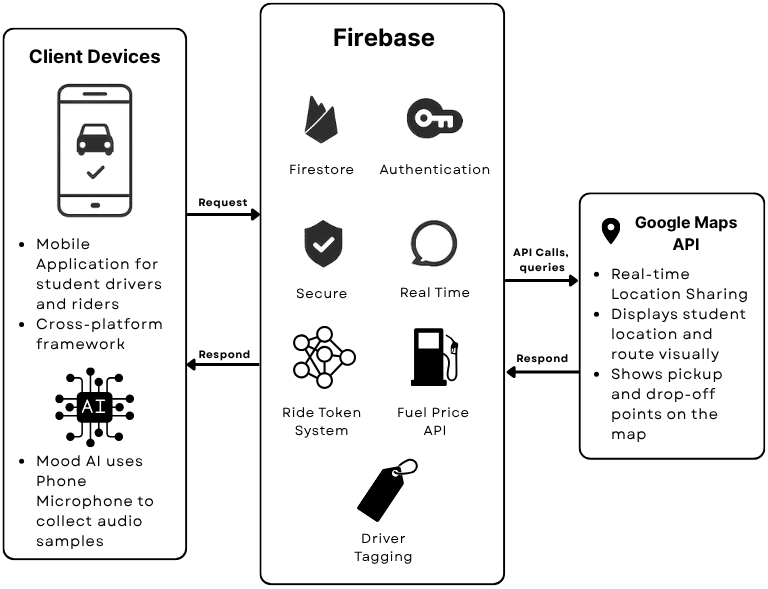
\includegraphics[width=0.54\textwidth]{images/conceptual.png} % Adjust width as needed
    \caption{Conceptual Framework}
    \label{fig:conceptual}
\end{figure}

SanCarGo is a mobile ridesharing system designed to connect student-drivers and student-passengers traveling to or from the Bunzel Building at the University of San Carlos Talamban Campus (USC-TC). The system uses the user’s location, trip direction, selected ride points, available vehicle capacity, and the passenger's mood and vehicle preferences to support route planning and ride-request processing. Its outputs include a displayed route, ride-request status, match information, and trip updates.

The application was developed using Flutter for Android and iOS. Firebase Authentication manages user sign-in, while administrative approval and role-based checks govern access to ride functions. Cloud Firestore stores application data, including user profiles, ride requests, driver availability, and ride records. Firebase Cloud Functions perform server-side operations such as creating requests and accepting rides. Google Maps displays locations and routes, while routing services provide route geometry and travel estimates.

The system was designed to accommodate routes and ride points beyond USC-TC. However, for this study, testing and demonstration are limited to selected points within the campus. The Bunzel Point serves as the fixed campus terminal and lies inside the operational geofence. The remaining study points lie outside that geofence but within USC-TC.


An additional layer of personalization is introduced through a Mood-Based AI system. This system rates the energy of the sound in the car, whether music or speech, as Lively, Calm, or Quiet, using two small pretrained models that run on the driver's phone and two lightweight arousal heads. Passengers indicate the moods they accept when they request a ride, and the system incorporates this input during the driver-passenger matching process. This enhances comfort, improves rider satisfaction, and supports better ride experience alignment.

The Ride Token and CES point system (Section~\ref{sec:tokens}) rewards student drivers for completed rides with non-monetary incentives, fostering engagement and volunteerism.

For real-time communication, Firebase Cloud Messaging facilitates immediate and reliable exchange of information between riders and drivers, such as ride requests and acceptance confirmations.


\section{System Features}

SanCarGo provides features for requesting, coordinating, and monitoring shared rides within a restricted student community:
\begin{itemize}
    \item \textbf{Ride requests and acceptance}: Passengers request a ride using designated ride points. Available drivers can review and accept eligible requests, subject to server-side checks.
    \item \textbf{Trip-direction classification}: The application classifies trips as inbound or outbound according to the user’s position relative to the Bunzel Building geofence.
    \item \textbf{Route generation and rerouting}: The application displays a route between the trip’s origin and destination and requests an updated route when the driver deviates sufficiently or moves a specified distance.
    \item \textbf{Ride-point matching}: The driver interface compares relevant ride points with the remaining route. Acceptance is subject to additional checks, including proximity to the pickup point, capacity, direction, and queue order.
    \item \textbf{Location tracking}: During a trip, location updates support route display and allow a matched passenger to follow the driver’s position.
    \item \textbf{Notifications and chat}: The application provides push notifications for selected ride events and an in-app communication channel for matched users. Availability depends on device configuration and connectivity.
    \item \textbf{Destination selection and early drop-off}: For an outbound trip, the driver can select a destination through place search or a map pin. A passenger may request an early drop-off for the driver to confirm.
    \item \textbf{Ride history, feedback, and reports}: Users can review ride records and submit ratings or reports through the application.
    \item \textbf{Mood-based matching}: Passengers choose the moods they accept, and the driver's phone rates the sound in the car as Lively, Calm, or Quiet (Section~\ref{sec:ai}). The mood is applied as a filter when a driver accepts a request.
    \item \textbf{Ride Tokens and CES points}: For student drivers, the system tracks accumulated Ride Tokens and converts them into CES points (Section~\ref{sec:tokens}), which rewards their contribution to shared transportation.
    \item \textbf{Emergency alert}: The application provides an alert that records the event and notifies administrators. It should not be described as a direct connection to emergency responders.
    \item \textbf{Account verification and administration}: Registration requires verification and administrative review. Administrators can review registrations, manage users and ride points, review Ride Token claims, set the fuel price and semester period that drive the Ride Token system, and examine reports and ride records.
    \item \textbf{Connectivity and error handling}: The application indicates loss of connectivity and records supported errors through Firebase Crashlytics. Server-dependent actions, including request creation and acceptance, require a connection.
\end{itemize}
These features support ride coordination and administrative oversight. Their presence alone does not establish improved safety, reduced emissions, or reduced travel costs; such outcomes require separate evidence.


\section{User Roles}

SanCarGo defines three principal user roles: passenger, driver, and administrator. Access to functions and data is governed by authentication, approval status, role checks, and the applicable Firebase Security Rules. Table~\ref{tab: user roles} shows the features each role can access, and Figure~\ref{fig: use case} shows the use cases.

{
\renewcommand{\arraystretch}{1.25}
\begin{longtable}{|>{\raggedright\arraybackslash}p{6.2cm}|c|c|c|}
\caption{User Types and their Feature Access}\label{tab: user roles}\\
\hline
\textbf{Feature} & \textbf{Passenger} & \textbf{Driver} & \textbf{Admin} \\
\hline
\endfirsthead
\multicolumn{4}{l}{\small\textit{Table 3.1 (continued)}}\\
\hline
\textbf{Feature} & \textbf{Passenger} & \textbf{Driver} & \textbf{Admin} \\
\hline
\endhead
\hline
\endfoot
User Registration and Login  & \cmark & \cmark & \cmark \\ 
        USC Email Verification  & \cmark & \cmark & \cmark \\ 
        Profile Management  & \cmark & \cmark & \cmark \\ 
        Request a Ride  & \cmark & \xmark & \xmark \\ 
        Accept/Reject Ride Requests  & \xmark & \cmark & \xmark \\ 
        Notification of Match  & \cmark & \cmark & \xmark \\ 
        Live Ride Tracking & \cmark & \cmark & \xmark \\ 
        Navigation Assistance (Google Maps API) & \cmark & \cmark & \xmark \\ 
        Ride Token Earning System & \xmark & \cmark & \xmark \\ 
        Ride Review and Rating & \cmark & \cmark & \xmark \\  
        In-App Chat with Matched User & \cmark & \cmark & \xmark \\ 
        Emergency Alert Button & \cmark & \cmark & \xmark \\ 
        Mood Preference Selection & \cmark & \xmark & \xmark \\ 
        AI Mood Detection (Music-Based) & \xmark & \cmark & \xmark \\ 
        Mood-Based Matching System & \cmark & \cmark & \xmark \\ 
        
        Approve/Deny Registrations & \xmark & \xmark & \cmark \\ 
        Manage Rides and Users & \xmark & \xmark & \cmark \\ 
        Review Ride Token Claims & \xmark & \xmark & \cmark \\ 
        Manage Ride Points, Fuel Price, and Semester Period & \xmark & \xmark & \cmark \\ 
        View Ride Logs and Transaction History & \cmark & \cmark & \cmark \\ 
        Suspend/Remove Users & \xmark & \xmark & \cmark \\ 
        Generate User Reports & \xmark & \xmark & \cmark \\
\end{longtable}
}

Passenger. A passenger can submit a ride request, select an available ride point, the moods they accept, and a vehicle preference, monitor the request, view the matched driver’s location during the trip, communicate with the driver, and provide feedback or submit a report.

Driver. An approved driver can specify availability and passenger capacity, select an outbound destination when applicable, view eligible requests, accept requests, and manage pickup and trip completion. A driver can earn Ride Tokens for completed rides and can also communicate with matched passengers and submit feedback or reports.

Administrator. An administrator reviews registration submissions and supporting documents, manages users and approved ride points, and reviews operational records and reports. Administrative permissions allow access to information needed for these tasks and should be restricted to authorized accounts.

A role-based design limits access according to the operation and record involved; it does not eliminate the need to test the rules and review their deployed configuration.

\begin{figure}[htbp]
    \centering
    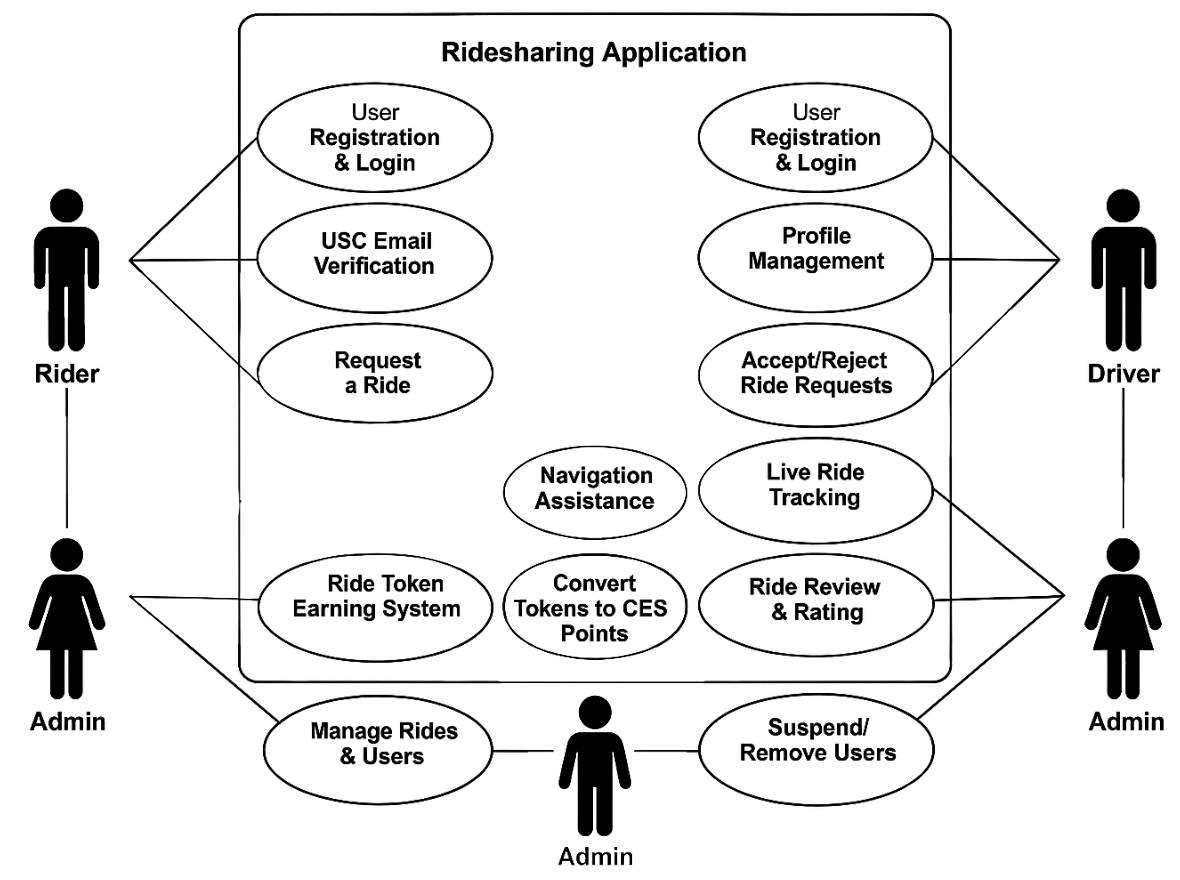
\includegraphics[width=0.75\textwidth]{images/use case.png}
    \caption{Use case diagram of the ridesharing application}
    \label{fig: use case}
\end{figure}

\section{Software Framework and Tools}
\label{sec:tools}

SanCarGo follows a client-server architecture. The Flutter mobile application provides the user interface, location and map interactions, while Firebase services support authentication, data storage, server-side processing, and notifications.
Table~\ref{tab: tools} lists the tools and technologies used.

\begin{table}[htbp]
    \centering
    \caption{Development Tools and Technologies}
    \small
    \renewcommand{\arraystretch}{1.2}

    \begin{tabular}{|>{\raggedright\arraybackslash}p{0.20\textwidth}|>{\raggedright\arraybackslash}p{0.26\textwidth}|>{\raggedright\arraybackslash}p{0.45\textwidth}|}
        \hline
        \textbf{Component} & \textbf{Technology Used} & \textbf{Justification} \\ 
        \hline
        Frontend & Flutter (Dart) & Cross-platform development (iOS \& Android) \\ 
        
        Backend & Firebase Firestore & Stores ride requests, user information, location data, tokens, weekly fuel price data, and route history in real-time. \\ 

        Authentication & Firebase Auth & Secure login with USC email verification \\ 
        
        Mapping \& GPS & Google Maps SDK; Google Routes API (through a Cloud Function), with OSRM as fallback; Google Places API (New) & Map display and location tracking on the device; route geometry, distance, and duration computed on the server so the API key stays out of the app; typed destination search. \\ 
        
        Proximity Detection \& Matching & Firebase Cloud Functions & Classify trip direction, create ride requests, perform the server-side checks when a driver accepts a request, calculate Ride Tokens, and refresh the fuel price. \\ 

        Notifications & Firebase Cloud Messaging & Push alerts for requests, ride status, chat messages, and administrator decisions. \\ 

        Reliability \& Security & Firebase Crashlytics, connectivity\_plus, Firebase App Check, Firebase Security Rules & Crash reporting, offline indicator, app verification, and role-based access to data and uploaded documents. \\ 
        
        Mood-Based AI System & YAMNet (TensorFlow Lite) + x-vector (ONNX) + Firebase & Rates the arousal of the sound in the driver's car as Lively, Calm, or Quiet. YAMNet tells speech, music, and neither apart, and a speech head or a music head rates the arousal. Matching is improved by aligning the driver's mood label with the rider's preference. \\ 
        
        Audio Processing & Google Colab (training of the heads) and on-device inference in Flutter & The heads are trained in Colab on RAVDESS and DEAM and exported as small files. On the device, 5.295-second windows of 16~kHz audio are converted in memory and passed to the models. \\      
        
        Model Deployment & TensorFlow Lite and ONNX models, and head files, bundled with the app & Allows on-device inference with no connection. The models ship inside the application, so updating them requires an app update. \\ 

                Pre-release Distribution & Firebase App Distribution & Delivers Android test builds to invited UAT testers by email, without an app store listing (Section~\ref{sec:distribution}). Android Studio and Xcode build and install the Android and iOS apps directly on testing devices (Section~\ref{sec:install}). \\

        \hline
    \end{tabular}
    \label{tab: tools}
\end{table}

Android builds for user acceptance testing are delivered through Firebase App Distribution (Section~\ref{sec:distribution}), and other builds are installed directly from Android Studio and Xcode (Section~\ref{sec:install}).

The exact availability of platform services and notifications should be reported according to the devices and configurations used during testing.


\section{Mood-based AI Matching System}
\label{sec:ai}
A mood-based artificial intelligence (AI) is integrated into ride matching. It listens to the sound inside the driver's vehicle on the driver's phone, reports one label at a time, and the label is matched with the moods that the passenger accepts. This section presents the AI from the requirements and the theoretical design down to its implementation, and then the plan for evaluating it. The results are in Section~\ref{sec:ai-results}. The backend and device architecture are in Section~\ref{sec:tools}.

\subsection{Purpose and Requirements}
\label{sec:ai-purpose}
The AI rates the arousal, which is the energy, of the sound inside the vehicle and reports it as one of three moods. In this study, mood refers to the energy of the sound and not to the emotional state of a driver or passenger, and the AI does not judge anyone's mood.
\begin{itemize}
    \item \textbf{Lively:} high-energy music or speech.
    \item \textbf{Calm:} low-energy music or speech.
    \item \textbf{Quiet:} no music or speech event, such as silence, engine noise, air-conditioner noise, or passing traffic.
\end{itemize}
Passengers choose the moods they accept according to the ride they want: Quiet for a silent ride, for example to study; Calm for calm music or soft talk; and Lively for high-energy music or talk. These ride atmospheres are assumptions of the proponents, because no survey of music preferences was conducted. They are consistent with the studies in Section~\ref{sec:lit-music}~\cite{north2004uses,constine2019uber}. Speech receives a mood in the same way as music, because a driver may play a podcast or talk radio, and a car with a podcast would otherwise read as Quiet and be matched with a passenger who wants a quiet ride. The definitions rest on the studies of Chapter~2 and on the measurements of Chapter~4, because no external experts were available. From these purposes, the AI must meet the requirements in Table~\ref{tab:ai-req}.

\begin{table}[htbp]
    \centering
    \caption{Requirements of the mood AI}\label{tab:ai-req}
    \small
    \renewcommand{\arraystretch}{1.2}
    \begin{tabular}{|c|>{\raggedright\arraybackslash}p{.80\textwidth}|}
        \hline
        \textbf{No.} & \textbf{Requirement} \\
        \hline
        R1 & Rate the energy of the sound in the car as Lively, Calm, or Quiet. \\
        \hline
        R2 & Rate music and speech on the same axis. \\
        \hline
        R3 & Run on the driver's phone and work without an internet connection. \\
        \hline
        R4 & Keep the audio on the phone: listen only while the driver is available, never on a motorcycle, and store and send only the mood label. \\
        \hline
        R5 & Follow the sound of the car without the label flickering. \\
        \hline
        R6 & Never stop a ride: an unknown or missing label must not block a match. \\
        \hline
    \end{tabular}
\end{table}

\subsection{Theoretical Design}
\label{sec:ai-theory}
\textbf{Why audio.} The sound in the car was chosen as the matching attribute for three reasons. The driver's phone can sense it automatically while the driver is available, without extra input. It can be processed on the phone, so no recording is stored or sent, which fits the on-device approach reviewed in Section~\ref{sec:lit-ondevice}~\cite{zhao2022survey}. Small models can classify it within mobile constraints~\cite{lane2015deep}. A driver-chosen tag would be simpler, but it depends on the driver remembering to update it and reporting it honestly, whereas audio reflects what is playing at the time.

\textbf{Why arousal.} Studies of affect, environments, and music describe sound on an arousal axis~\cite{russell1980circumplex,russell1980environments,panda2023audio}, and no study gives loudness or tempo cutoffs for a vehicle (Section~\ref{sec:lit-audio}). Arousal also applies to speech and music alike (R2).

\textbf{Why three moods.} The proponents weighed three levels against two levels, four or five levels, music genres, emotion categories such as happy and sad, and a continuous energy score. Three levels were chosen for four reasons.
\begin{enumerate}
    \item \textbf{A passenger must find a driver quickly.} The more moods there are, the fewer available drivers fall in each one, so the chance that at least one matches a passenger falls. This is the principle of thickness~\cite{roth2008market}. Table~\ref{tab:ai-chance} shows the effect when the drivers are spread evenly over the moods and the passenger accepts one mood. The values are illustrative, since real tastes are uneven, and a passenger can also select more than one mood or No Preference, which raises the chance.
    \item \textbf{People agree less on finer categories.} Agreement falls as mood categories become finer~\cite{hu2008mirex,gomez2019emotions}, and low agreement limits how well a model can match human ratings.
    \item \textbf{Small mood sets are standard.} The studies of Section~\ref{sec:lit-music} used small sets of mood clusters~\cite{hu2008mirex,hu2007simplified}.
    \item \textbf{Each level matches a passenger's choice.} Two levels would place a silent ride and calm sound together, so a passenger who wants silence could be matched with a driver who plays music or talk.
\end{enumerate}

\begin{table}[htbp]
    \centering
    \caption{Chance that a passenger finds at least one matching driver, $1-(1-1/k)^n$ for $n$ available drivers and $k$ moods}\label{tab:ai-chance}
    \small
    \renewcommand{\arraystretch}{1.2}
    \begin{tabular}{|l|c|c|c|}
        \hline
        \textbf{Moods ($k$)} & \textbf{3 drivers} & \textbf{5 drivers} & \textbf{10 drivers} \\
        \hline
        2 & 88\% & 97\% & 99.9\% \\
        \hline
        3 (this study) & 70\% & 87\% & 98\% \\
        \hline
        5 & 49\% & 67\% & 89\% \\
        \hline
        10 (for example, genres) & 27\% & 41\% & 65\% \\
        \hline
    \end{tabular}
\end{table}

Genres were rejected because they split the drivers into groups that are too small (Table~\ref{tab:ai-chance}) and a genre is not the same as energy. Emotion categories describe people, which a microphone cannot measure. A continuous energy score is harder for a passenger to choose from and is left for future work.

\textbf{Two stages, one head for each kind of sound.} A model of arousal transfers within one kind of sound but largely fails across kinds of sound~\cite{zhang2026generalisation}, and arousal is shared between speech and music only in part~\cite{coutinho2014transfer}. The design therefore first tells what kind of sound a window holds, and then applies the arousal head of that kind, so that each head is used only on the kind of sound it was trained on.

\textbf{A stable label.} Rating one window at a time gives a label that can flip on a single odd window. The stored label therefore changes only after two identical new labels in a row, a simple form of the two-threshold rule that is used to stop unstable labels from flipping~\cite{cances2019postprocessing}.

\textbf{A fail-open filter.} The AI is an optional layer on the ridesharing function, so it must not be able to stop a ride (R6). A request is refused on mood grounds only when the driver's label is known and the passenger has chosen a mood set that does not include it. Excluding every driver whose label is unknown would block rides whenever the classifier is unsure or the microphone is unavailable, and it would thin the pool of drivers. Ranking compatible drivers higher would limit the cost of a wrong label, but it would show passengers drivers whose mood they did not choose, so it is recommended for future work (Section~\ref{sec:recs}).

\subsection{System Overview}
\label{sec:ai-overview}
Figure~\ref{fig:ai-flow} shows the flow. The microphone gives a continuous stream that is cut into windows. For each window, the sound-type step decides between speech, music, and neither (Section~\ref{sec:ai-window}). The head of that kind of sound gives an arousal reading and a cutoff turns it into Lively or Calm (Section~\ref{sec:ai-heads}). The confirm rule updates the stored label, which is saved in the driver's availability record (Section~\ref{sec:ai-runtime}). The matchRide function compares the stored label with the moods the passenger accepts (Section~\ref{sec:moodmatch}). Everything before the saved label runs on the phone.

\begin{figure}[htbp]
    \centering
    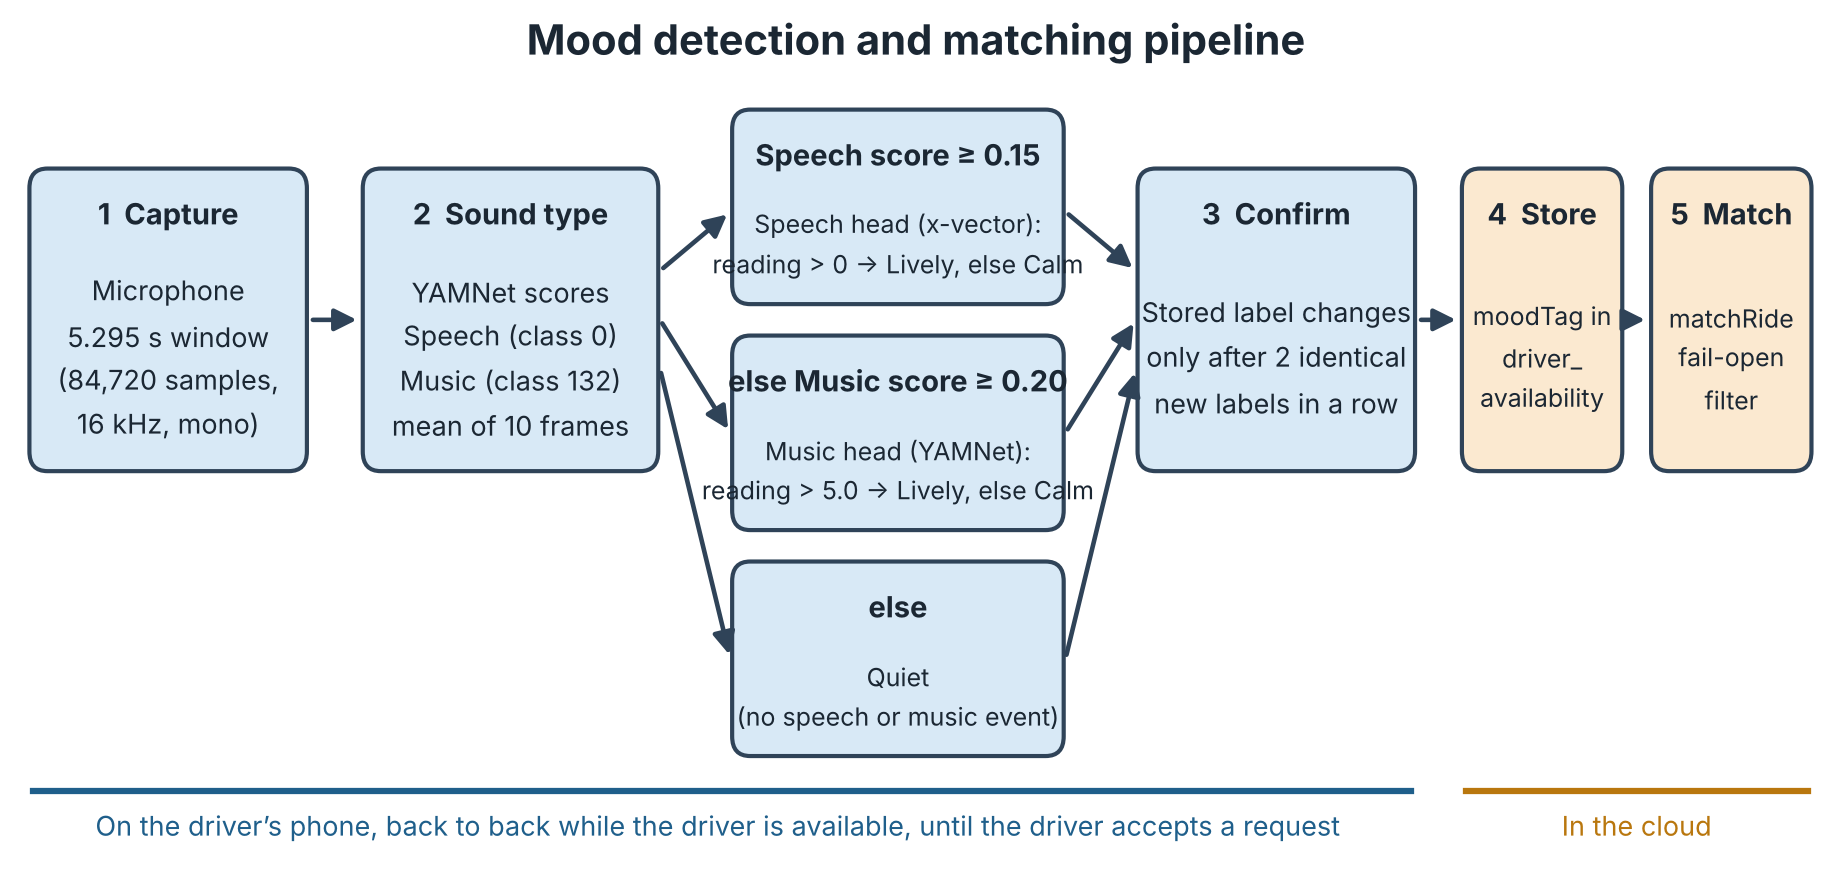
\includegraphics[width=1.0\textwidth]{images/ai_flow.png}
    \caption{Flow of the mood AI from the microphone to the matching function.}
    \label{fig:ai-flow}
\end{figure}

The basis of every value is stated where it is introduced as a study, a range that studies give, or a choice of the proponents with its reason, because studies justify methods and axes far more often than exact constants such as window lengths and cutoffs.

\subsection{Data Sources}
\label{sec:ai-data}
The AI uses two pretrained models and two small heads that the proponents trained. YAMNet~\cite{plakal2019yamnet}, a sound-event model trained on AudioSet~\cite{gemmeke2017audioset}, and an x-vector speaker-recognition model~\cite{snyder2018xvectors} were not trained by the proponents. The heads were trained on the data of Table~\ref{tab:ai-sources}, and the other sets were used only for tuning and testing.

\begin{table}[htbp]
    \centering
    \caption{Data sources and their use}\label{tab:ai-sources}
    \small
    \renewcommand{\arraystretch}{1.2}
    \begin{tabular}{|>{\raggedright\arraybackslash}p{.17\textwidth}|>{\raggedright\arraybackslash}p{.15\textwidth}|>{\raggedright\arraybackslash}p{.46\textwidth}|>{\raggedright\arraybackslash}p{.12\textwidth}|}
        \hline
        \textbf{Use} & \textbf{Source} & \textbf{Content} & \textbf{Licence} \\
        \hline
        Speech head, training & RAVDESS~\cite{livingstone2018ravdess} & 1,440 speech files from 24 actors; 1,248 clips are used after the calm clips are left out & CC BY-NC-SA 4.0 \\
        \hline
        Music head, training & DEAM~\cite{aljanaki2017deam} & 1,744 excerpts of 45 seconds, cut into 15,696 windows of 5.295 seconds (about 9 for each song), each labeled with the mean arousal of its song on a scale of 1 to 9 & CC BY-NC-SA 4.0 \\
        \hline
        Music head, held-out test & PMEmo~\cite{zhang2018pmemo} & 767 chorus clips, never used for training & CC BY-NC-SA 4.0 \\
        \hline
        Sound-type cutoffs, mixing, and noise tests & MUSAN~\cite{snyder2015musan} & Speech, music, and noise recordings, with no arousal ratings, so it was not used to train a head & CC BY 4.0 \\
        \hline
    \end{tabular}
\end{table}

DEAM supplies music that people rated for arousal, and RAVDESS supplies speech by actors who read two fixed sentences in several emotions (Section~\ref{sec:lit-audio}). RAVDESS is acted speech and not natural speech, which is a limit of the speech head (Section~\ref{sec:ai-limits}). The best-matching speech data, MSP-Podcast, needs an agreement signed by an institution, and the proponents did not pursue it. PMEmo is licensed for non-commercial use only, which fits a non-commercial thesis, and it is used for evaluation only. The audio of the sets is not part of the application.

\subsection{Window and Sound-Type Step}
\label{sec:ai-window}
\textbf{Window.} The AI rates one window of audio at a time. A window is 84,720 samples at 16~kHz, which is 5.295 seconds and exactly 10 YAMNet frames (each 0.975 seconds long, with a new one every 0.48 seconds), the window on which the cutoffs of the sound-type step were tuned. It is slightly above the range of 1 to 5 seconds that studies report for arousal~\cite{sun2023segmented}, so its basis is a range from a study, set together with the update interval (Section~\ref{sec:ai-results}), and not a value that a study proves best. Windows follow each other back to back.

\textbf{Sound type.} YAMNet scores the window and gives, for each of its 10 frames, a score for each of its 521 sound classes and an embedding of 1,024 numbers. The speech score is the mean over the frames of class 0 (Speech), and the music score is the mean of class 132 (Music). A window holds speech when the speech score is at least 0.15, and music when the music score is at least 0.20. The cutoffs were found by a search on MUSAN tuning data, in line with the practice of setting thresholds on validation data~\cite{cances2019postprocessing}, and they lie on a plateau: any value from 0.10 to 0.30 scored within 0.01 of the best (Section~\ref{sec:ai-results}). The YAMNet file that runs in the application is a TensorFlow Lite model of 15.0~MB that uses only the built-in operations of the runtime.

\textbf{Decision rule.} Speech is checked first:
\begin{enumerate}
    \item If the speech score is at least 0.15, the speech head decides, and the label is Lively or Calm.
    \item Otherwise, if the music score is at least 0.20, the music head decides, and the label is Lively or Calm.
    \item Otherwise, the label is Quiet.
\end{enumerate}

\textbf{Mixed audio.} The pipeline does not separate one source from the other. When a window holds both, the speech is rated and the music is not. The order is a choice of the proponents. No study measures which source should be rated when both are clearly audible, and the literature gives only indirect support: listeners rank speech among the most important sounds, and models built for a single source fail on mixtures~\cite{liu2025salience,laugs2020mixed}. Music that is more than 36.4~dB below the speech is treated as inaudible, following the lowest level at which background music was still barely audible in television~\cite{batlleroca2023background}.

\subsection{Arousal Heads}
\label{sec:ai-heads}
\textbf{Form.} Each head is a linear layer on a frozen embedding, which is the standard way to use a pretrained embedding~\cite{niizumi2023byola,koh2021embeddings}. A head reads the embedding $x$ of a window and gives one arousal reading $r$ as in Equation~(\ref{eq:head}), where $x_j$ is feature $j$ of the embedding, $\mu_j$ and $s_j$ are the mean and the scale of that feature in the training data, $w_j$ is its coefficient, and $b$ is the intercept. Both heads compute the same sum, and only their numbers differ.
\begin{equation}\label{eq:head}
    r = b + \sum_j \frac{x_j - \mu_j}{s_j}\, w_j
\end{equation}

\textbf{Training.} Training was done in Google Colab, and the numbers were exported to files that the application bundles. Each head is a regularized linear regression, trained on labels that people or published anchors give, so nothing in the AI is clustered or learned without labels.

\textbf{Speech head.} The embedding is the 512 numbers that the x-vector model gives for the raw audio of one window. The x-vector was chosen because speaker-recognition embeddings beat YAMNet for emotion categories~\cite{phukan2023embeddings}, and the choice was checked against two other embeddings (Section~\ref{sec:ai-results}). The head was trained on the 1,248 RAVDESS clips that remain after the calm clips are left out, with a regularization strength of 100. Each emotion was turned into an arousal value with the anchors of Zhou et al.~\cite{zhou2023arousal}: angry 0.59, fearful 0.60, happy 0.51, disgust 0.35, sad $-0.27$, surprised 0.67, and neutral 0. RAVDESS calm has no published anchor, so those clips were left out and no value was invented for them. The cutoff is 0, the neutral origin of the axis: a reading above 0 is Lively and any other reading is Calm. Validation leaves one actor out at a time~\cite{antoniou2023speech}, so no actor in a test was seen in training.

\textbf{Music head.} The embedding is the 1,024 numbers of each of the 10 YAMNet frames of a window, pooled over the frames by the mean and by the maximum, which gives 2,048 numbers with the mean first~\cite{koh2021embeddings}. The head was trained on the 15,696 DEAM windows, each labeled with the mean arousal of its song, with a regularization strength of 1,000. The windows have the same length as the windows that the application rates. The cutoff is 5.0, the midpoint of the scale of 1 to 9: a reading above 5.0 is Lively and any other reading is Calm. It is a working value of the proponents (Sections~\ref{sec:ai-results} and~\ref{sec:ai-limits}). Validation uses 10 folds in which whole songs are held out, so the windows of one song never sit on both sides of a split.

\subsection{Runtime Classification and Driver Tagging}
\label{sec:ai-runtime}
\textbf{Pipeline.} The whole classifier runs on the driver's phone, in Flutter, and only a mood word is sent to the server. The application cuts the audio stream into windows, converts each to numbers in memory, runs YAMNet and, when speech is present, the x-vector model, and applies the heads and the decision rule. If the previous window is still being analyzed, the next one is skipped. After an error in the stream, the application tries again after 5 seconds. If the driver denies the microphone permission, the application stops trying and no label is produced, but the driver can still go available.

\textbf{Confirm rule.} The label of each window is the raw label. The stored label changes only after two identical new raw labels in a row. The first raw label is taken as it is, so the screen shows ``Sensing mood'' until the first window is finished. The value of two comes from a simulation (Section~\ref{sec:ai-results}) with a target that the proponents set, and not from a study.

\textbf{When the microphone is on.} The microphone is used only while the driver is marked available, started and stopped by the Available switch. It is never used for motorcycle drivers, because a motorcycle has no cabin to sample: no permission prompt appears and no label is written. A passenger who prefers motorcycles sees a short note in place of the mood selector, and the preference is stored as Any.

\textbf{Accept lock.} The group decided that the driver is locked to one mood, so that every passenger in the car shares the same mood preference. The lock starts when the driver accepts a request and not at pickup, so the mood that matched the first passenger cannot drift before pickup and hide the next passenger who wanted the same mood. When the lock starts, the microphone stops and the stored label stays as it was for the rest of the trip. If the driver cancels every accepted request before confirming a pickup, the lock is lifted and the microphone senses a mood afresh. Cancelling one of two accepted passengers keeps the lock, and if an accept fails, the microphone resumes. When the driver goes offline, the availability record is deleted, and a new session starts at ``Sensing mood''.

\textbf{What is stored and sent.} One field is written to the driver's availability record in Firestore (Section~\ref{sec:tools}): the label, stored as \texttt{loud}, \texttt{chill}, or \texttt{quiet} for Lively, Calm, or Quiet, with the time it was updated, and only when the confirmed label changes. The raw audio, the features, and the embeddings are never written to disk or uploaded. A driver who is not available has no record (UNAVAILABLE). A driver who is available but has not yet received a label has a record with no label (UNCLASSIFIED). The record is recreated each time a driver goes available, so a label from an earlier trip is never carried over.

\textbf{Consent.} Before the operating system asks for microphone access, the application shows a plain-language dialog. It says that the application analyzes clips of about 5 seconds, that the microphone indicator stays on, including in the background, that the audio is analyzed on the phone and never recorded, saved, or uploaded, that the microphone can hear conversation in the car, and that only the mood word leaves the phone. A separate notice, ``Your music may be interrupted'', appears when the driver starts a ride. It says that the microphone can pause or lower the music, especially over Bluetooth, that the mood is locked once the driver accepts a passenger, and that the audio is processed on the phone and never uploaded.

\textbf{Platform behavior.} Table~\ref{tab:ai-mic} gives how the microphone is handled on each platform. The pause of the music on iPhone is a known limitation that is reduced and not removed (Section~\ref{sec:ai-limits}).

\begin{table}[htbp]
    \centering
    \caption{Microphone handling on each platform}\label{tab:ai-mic}
    \small
    \renewcommand{\arraystretch}{1.2}
    \begin{tabular}{|>{\raggedright\arraybackslash}p{.17\textwidth}|>{\raggedright\arraybackslash}p{.73\textwidth}|}
        \hline
        \textbf{Platform} & \textbf{Behavior} \\
        \hline
        Android & Runs as a foreground service of the microphone type, and the microphone is closed during any rest between windows. \\
        \hline
        iPhone & The audio session is set to play and record, mixed with other audio, and the stream stays open between windows. It needs iOS 16 or later, because the runtime of the speech model requires it. \\
        \hline
        iPhone music & Other audio that is playing pauses for less than a second when the microphone starts and again when it stops, and then resumes by itself. After the microphone stops, the application tells other apps that it has released the audio session, which lets the music resume. \\
        \hline
    \end{tabular}
\end{table}

\subsection{Matching with the Passenger's Preference}
\label{sec:moodmatch}
When requesting a ride, passengers select the moods they accept (any combination of Lively, Calm, and Quiet) or choose No Preference, which is stored as an empty list, with the ride request in Firestore. Mood is applied as a fail-open filter at the point of acceptance. When a driver accepts a request, the matchRide Cloud Function checks the request against the driver's stored label, using data it reads itself. A request is refused on mood grounds only when the passenger has chosen a specific subset of moods and the driver's label is known and outside that subset. A passenger with No Preference or all three moods selected, and any driver whose label is missing or unreadable, always passes. A wrong label can therefore delay a match for a passenger with a specific preference, but an unknown label never blocks one. The driver's screen applies the same check to decide which requests to show.

Table~\ref{tab:ai-accept} gives the checks that matchRide makes, in order, when a driver accepts a request. The first check that is not met rejects the acceptance. The vehicle-type preference of the passenger is applied with the same fail-open rule as mood. The checks marked HF are the hard filters of the use-case catalogue. Route alignment (HF-3) is applied on the driver's screen as a display filter, because the server stores the driver's location but not the route, so a request is shown only when its pickup lies within the route-match distance of the remaining route (Table~\ref{tab:rules-by-setting}).

{
\small
\setlength{\tabcolsep}{4pt}
\renewcommand{\arraystretch}{1.2}
\begin{longtable}{|>{\raggedright\arraybackslash}p{.16\textwidth}|>{\raggedright\arraybackslash}p{.50\textwidth}|>{\raggedright\arraybackslash}p{.24\textwidth}|}
\caption{Conditions checked when a driver accepts a request}\label{tab:ai-accept}\\
\hline
\textbf{Check} & \textbf{Condition to pass} & \textbf{Result if not met} \\
\hline
\endfirsthead
\hline
\textbf{Check} & \textbf{Condition to pass} & \textbf{Result if not met} \\
\hline
\endhead
\endfoot
Request state (HF-7) & The request is still pending, is not the driver's own, and was made in the current request format. & Rejected \\
\hline
Request data & The request has a valid direction (inbound or outbound) and a valid pickup coordinate. & Rejected \\
\hline
Driver state (HF-1, HF-2) & The driver is approved and not suspended, is available on the same direction as the request, and has a known location. & Rejected \\
\hline
Campus fence & An inbound driver is off campus, and an outbound driver is on campus. & Rejected \\
\hline
Seats (HF-4) & At least one passenger seat remains. & Rejected \\
\hline
Distance (HF-5) & The driver is within the acceptance distance of the pickup point in a straight line (Table~\ref{tab:rules-by-setting}). & Rejected \\
\hline
Mood & The passenger's accepted moods are empty or include all three (Any), or the driver's label is unknown, or the label is on the passenger's list. & Rejected only when the label is known and not on a partial list \\
\hline
Vehicle & The passenger has no preference, or the driver's vehicle kind is unknown, or it is the kind the passenger asked for. & Rejected only when the kind is known and different \\
\hline
Queue & The request is the oldest pending request at its queue point (first in, first out). & Rejected \\
\hline
Destination & For an outbound trip, the driver has chosen a final destination. & Rejected \\
\hline
\end{longtable}
}

Requests are served first-in, first-out. A passenger's place in the queue is fixed by the time the passenger first joined and never resets when the passenger edits their preferences. Passengers cannot widen their own mood selection, because free multi-selection weakens match quality. Instead, if no match is found after roughly two minutes, the system prompts the passenger to accept additional moods, and the search continues with the wider set.

\subsection{Evaluation Plan}
\label{sec:ai-eval}
Table~\ref{tab:ai-verify} states how each requirement is verified, and Table~\ref{tab:ai-tests} gives the data and the method of each test. The results are in Section~\ref{sec:ai-results}. Where a published figure exists, it is reported beside the result as a reference point and not as a target, because the data differ. The tests of the application and of the matching function are part of the testing plan in Section~\ref{sec:phases}.

\begin{table}[htbp]
    \centering
    \caption{Requirements and how each is verified}\label{tab:ai-verify}
    \small
    \renewcommand{\arraystretch}{1.2}
    \begin{tabular}{|c|>{\raggedright\arraybackslash}p{.46\textwidth}|>{\raggedright\arraybackslash}p{.34\textwidth}|}
        \hline
        \textbf{No.} & \textbf{Verified by} & \textbf{Results in} \\
        \hline
        R1 & Sound-type test, music head, speech head, rating check on car recordings & Sections~\ref{sec:ai-soundtype}, \ref{sec:ai-music}, \ref{sec:ai-speech}, and~\ref{sec:ai-rating} \\
        \hline
        R2 & Speech head, mixed audio & Sections~\ref{sec:ai-speech} and~\ref{sec:ai-mixed} \\
        \hline
        R3 & Models on the phones & Section~\ref{sec:ai-phones} \\
        \hline
        R4 & Flutter tests, system case S-F3 & Section~\ref{sec:ai-matchtests} \\
        \hline
        R5 & Simulation of the confirm rule and update interval & Section~\ref{sec:ai-confirm} \\
        \hline
        R6 & matchRide verification script, system case S-C5 & Section~\ref{sec:ai-matchtests} \\
        \hline
    \end{tabular}
\end{table}

{
\small
\setlength{\tabcolsep}{4pt}
\renewcommand{\arraystretch}{1.2}
\begin{longtable}{|>{\raggedright\arraybackslash}p{.12\textwidth}|>{\raggedright\arraybackslash}p{.22\textwidth}|>{\raggedright\arraybackslash}p{.36\textwidth}|>{\raggedright\arraybackslash}p{.20\textwidth}|}
\caption{Tests of the mood AI: data, method, and measures}\label{tab:ai-tests}\\
\hline
\textbf{Test} & \textbf{Data} & \textbf{Method} & \textbf{Measures} \\
\hline
\endfirsthead
\hline
\textbf{Test} & \textbf{Data} & \textbf{Method} & \textbf{Measures} \\
\hline
\endhead
\endfoot
Sound-type step & MUSAN. Cutoffs tuned on fma, librivox, and free-sound; tested on jamendo, rfm, hd-classical, fma-western-art, us-gov, and sound-bible, which were never used for tuning. & Windows of 1, 3, and 5 seconds, repeated with noise added at 20, 10, 5, and 0~dB. MUSAN noise is not the noise of a car. & Average of three recalls: speech, music, and neither. \\
\hline
Music head & DEAM, and the 767 PMEmo clips, which were never used for training. & 10 folds with songs held out; the reading of a song is the mean over its windows. Three heads at the cutoff of 5.0: the shipped head (trained and read on windows), a head trained on whole excerpts and read on the excerpt, and the same head read on windows. The cutoff of 5.0 assumes that the midpoints of the DEAM scale and the PMEmo scale (0.5) correspond. & Spearman correlation, Calm found, Lively found, balanced accuracy (their average), AUC on PMEmo, bootstrap intervals. \\
\hline
Speech head & RAVDESS, 24 actors; 150 MUSAN speech clips of 10 seconds for stability. & Leave one actor out~\cite{antoniou2023speech}. Three embeddings (x-vector, ECAPA, and YAMNet with the mean and the maximum), each with a linear head and with a small network of one hidden layer of 128 units. Stability: the first window, the last window, and their mean against the whole clip. & CCC with the anchors, averaged over the actors; Calm found; Lively found; balanced accuracy. Stability measures stability and not accuracy. \\
\hline
Mixed audio & 150 pairs of speech and music. & The music was mixed from 12~LU above the speech down to 36.4~dB below it, and the test was repeated with RMS in place of LU to check that the finding does not depend on the measure of loudness. & How often the sound-type step hears each source; how often adding one source changes the label of the head of the other; how often the two orders give different labels. \\
\hline
Confirm rule and update interval & Simulation from a saved pool of real window labels (below). & $N$ from 1 to 6, and update intervals of 5.295 and 10 seconds. & False flips, reversals, lag, accuracy. \\
\hline
Models on the phones & 10 golden clips, one Android phone, and one iPhone. & Converted models against the original models; the clips run through the application and compared with the notebook, with a tolerance of 0.001; live use in a quiet room, with music, and with speech. & Largest differences in scores, embeddings, and readings; time for each window. Timings are of debug builds and are not benchmarks. \\
\hline
Rating check & 30 recordings made inside a car (below). & Labels of the AI against the labels of two blind raters. & Cohen's kappa; Fleiss' kappa; share of agreed clips matched. \\
\hline
Matching and privacy & The matchRide function, the Flutter code, and the application. & The Cloud Functions verification script, the Flutter tests, and system cases S-C5 and S-F3. & Pass or fail of each check. \\
\hline
\end{longtable}
}

\textbf{Simulation of the confirm rule.} The confirm rule and the update interval were chosen with a simulation, in the manner of the trade-off method of Janko and Lu{\v{s}}trek~\cite{janko2021energy}, with accuracy and lag in place of energy because no energy was measured. The simulation works as follows.
\begin{itemize}
    \item \textbf{Timelines.} Each timeline lasts 1,200 seconds and is built from scenes of five kinds of sound: Lively speech, Calm speech, Lively music, Calm music, and Quiet. A scene lasts at least 10 seconds, with a length that follows a gamma distribution and averages 25, 60, or 120 seconds. 300 timelines were averaged for each setting.
    \item \textbf{Labels.} The raw labels are drawn from a saved pool of real window labels of the pipeline and passed through the confirm rule for $N$ from 1 to 6, with an update every 5.295 or 10 seconds. The truth of a scene is the reading of the pipeline on the clean clip and not a human rating.
    \item \textbf{Errors.} Errors are drawn in two ways that bracket the real car. Independent: each window is drawn on its own, the best case for the filter. By clip: one clip is used for a scene, so a clip that the pipeline gets wrong stays wrong for the whole scene, the worst case, which no value of $N$ can fix.
    \item \textbf{Metrics.} False flips for each minute (the stored label changes to a label that is not the true one), reversals for each hour (the label changes and returns to what it was within 60 seconds), lag in seconds from a real change until the stored label is right, and accuracy as the share of seconds in which the stored label is right.
    \item \textbf{Rule.} The smallest $N$ with at most 0.10 false flips for each minute, for independent errors, 60-second scenes, and updates every 5.295 seconds, fixed before the run.
    \item \textbf{Interval grid.} A separate grid compared update intervals of 5.295, 10, 15, 20, 30, 45, and 60 seconds with smoothing spans of 0, 15, 30, and 60 seconds and three two-threshold bands, over the same scene lengths. A bootstrap test with a 95\% interval was used to find the largest interval that is not clearly worse than the best.
\end{itemize}
The target of 0.10 (one false flip in ten minutes), the reversal window of 60 seconds, the scene lengths, and the 300 timelines are the proponents' own settings and not values from a study.

\textbf{Researcher rating check.} The final check compares the labels of the AI with the labels of people on recordings made inside a car. It is a sanity check and not ground truth: the researchers built the system, three raters are few, and no student ratings are part of the plan.
\begin{itemize}
    \item \textbf{Clips.} Thirty clips of 10 seconds were recorded: 16 of music, 11 of speech, and 3 of quiet. The music and the speech were drawn at random, with a fixed seed of 2026, from lists of popular songs and of podcasts, and each excerpt was taken from 1:00 of the song or 5:00 of the episode, so that it does not start on an intro. The quiet clips were recorded with the engine idling, the air conditioning on, and the road noise.
    \item \textbf{Recording.} The clips were played through the car stereo of the researcher over Bluetooth, and an iPhone 16 recorded them inside the car, in a cup holder behind the gear selector.
    \item \textbf{Raters.} Two research-team members who did not know the label of the AI rated each recording as Lively, Calm, or Quiet at home, with headphones and without talking to each other. The researcher who recorded the clips also rated them, but this rater was not blind, so that rater's results are supplementary. The primary result uses the two blind raters.
    \item \textbf{Analysis.} The label that both blind raters gave is the agreed label, and the label of the AI for a clip is the label of its first window of 5.295 seconds. Agreement between the raters is reported with Cohen's kappa, and the agreement of the three raters with Fleiss' kappa.
\end{itemize}

\subsection{Design Decisions and Refinements}
\label{sec:ai-choices}
Table~\ref{tab:ai-choices} lists each design decision, the alternatives that were weighed, and the reason. After reviewing the literature in Chapter~2, the proponents refined the design of the AI in several places, and each cell that begins with ``Proposal'' states what the proposal said. The proposal fixes no dataset or training detail, so these refinements concern the method and not any stated requirement. The last column says whether a choice comes from a study, sits within a range that studies give, or is a choice of the proponents with a reason. Evidence marked as a design reason was not tested.

{
\small
\setlength{\tabcolsep}{4pt}
\renewcommand{\arraystretch}{1.2}
\begin{longtable}{|>{\raggedright\arraybackslash}p{.14\textwidth}|>{\raggedright\arraybackslash}p{.26\textwidth}|>{\raggedright\arraybackslash}p{.17\textwidth}|>{\raggedright\arraybackslash}p{.33\textwidth}|}
\caption{Design decisions, alternatives, and refinements of the proposal}\label{tab:ai-choices}\\
\hline
\textbf{Aspect} & \textbf{Built system} & \textbf{Alternatives} & \textbf{Reason and basis} \\
\hline
\endfirsthead
\hline
\textbf{Aspect} & \textbf{Built system} & \textbf{Alternatives} & \textbf{Reason and basis} \\
\hline
\endhead
\endfoot
Names of the moods & Lively, Calm, Quiet (stored as loud, chill, quiet). Proposal: Loud, Chill, Quiet. & --- & The proponents judged that the new names better represent the mood. Decision of the proponents. \\
\hline
Definition of a mood & Perceived arousal of the sound. Proposal: loudness (70~dB and above, 50 to 70~dB) and tempo (120 and 100 beats per minute). & Loudness and tempo cutoffs, emotion categories & Arousal is the axis that studies of affect, environments, and music use, and no study gives dB or tempo cutoffs for a vehicle. Literature~\cite{russell1980circumplex,russell1980environments,panda2023audio}. \\
\hline
Matching attribute & In-car audio & Driver-chosen tag, driving style, ratings, music-app data, questionnaire & Automatic, private on the device, and describes the ride atmosphere directly. Design reason. \\
\hline
Where it runs & On the phone & Cloud server & No recording leaves the phone and no connection is needed. Literature~\cite{zhao2022survey}. \\
\hline
Number of moods & Three & Two, four or five, genres, emotions, continuous score & Larger matching pools, fewer disagreements, and a match with passenger choices. Table~\ref{tab:ai-chance}, \cite{hu2008mirex,hu2007simplified,gomez2019emotions,roth2008market}. \\
\hline
Features & Pretrained embeddings (YAMNet and an x-vector model). Proposal: amplitude, tempo, and timbre with Librosa MFCC. & --- & Pretrained models are small enough for a phone and have been tested on data that they were not trained on. Literature. \\
\hline
Structure & Sound type, then one head for each kind of sound. Proposal: one classifier. & One model for all sound & Arousal models fail across kinds of sound. Literature~\cite{zhang2026generalisation}. \\
\hline
Speech & Rated on the same axis as music. Proposal: no rule for speech. & --- & A car with talk only receives a label. Design reason. \\
\hline
Sound-type model and cutoffs & YAMNet; speech 0.15, music 0.20 & Other cutoffs, other models & Small enough for a phone, and the cutoffs lie on a plateau (0.10 to 0.30 scored within 0.01). Tested on MUSAN. \\
\hline
Speech embedding & x-vector with a linear head & ECAPA, YAMNet, small networks & Speaker-recognition embeddings beat YAMNet for emotion categories, and it scored best on CCC and balanced accuracy of the six variants. Literature~\cite{phukan2023embeddings}; tested. \\
\hline
Music embedding & YAMNet mean and maximum with a linear head & Whole-excerpt training & Pooling by mean and maximum works well, and the two training choices cannot be told apart at song level. Literature~\cite{koh2021embeddings}; tested. \\
\hline
Cutoffs of the heads & Speech 0; music 5.0 & Other values & Neutral is the origin of the axis, and 5.0 is the midpoint of the scale. Proponents' choice; working values. \\
\hline
Mixed audio & Speech first & Music first, rate both & Listeners rank speech highly, and the speech reading changes less when music is added. Indirect support~\cite{liu2025salience,laugs2020mixed}; tested. \\
\hline
Listening cycle & 5.295~s windows, back to back. Proposal: 10~s snippets with an update every 30~s. & 10~s, longer intervals & Equals 10 YAMNet frames and sits near a range that studies report, and accuracy fell with each longer interval in the simulation. Range from a study~\cite{sun2023segmented}; tested. \\
\hline
Stored label & Two identical labels in a row & Each window alone, larger $N$ & Cuts false flips about tenfold at a cost of about 5.8~s of lag. Simple form of~\cite{cances2019postprocessing}; simulation. \\
\hline
Timing of the mood & Locked when the driver accepts. Proposal: the mood may change during a trip. & Changes during the trip & Every passenger in the car shares one preference. Decision of the group. \\
\hline
Passenger's preference & Any set of moods; an empty set means Any. Proposal: one preferred mood, matched when the driver's tag equals it. & --- & Matching design of the group. \\
\hline
Use in matching & Fail-open filter & Always exclude on a mismatch, rank drivers & Cannot block a ride when the label is unknown or the passenger has no preference. Design reason. \\
\hline
Motorcycles & Never run the microphone. Proposal: treated like cars. & Treat like cars & No cabin to sample. Design reason. \\
\hline
\end{longtable}
}

\section{Routing System}
\label{sec:routing}

The routing system classifies trips relative to an operational polygon around the Bunzel Building. A user located inside or on the polygon is classified as outbound; a user outside the polygon is classified as inbound. This polygon is smaller than the USC-TC campus boundary. Consequently, a user may be outside the Bunzel geofence while still inside the campus.

Bunzel Point is the fixed terminal for the study: inbound requests end at Bunzel, while outbound requests begin there. The other points selected for testing and demonstration are USC TC Portal, SMED/Dorm, SAS, RH Building, LRC Building, MR Hall, SAFAD, and TC Church. These points are within USC-TC but outside the Bunzel geofence.

The application maintains a local copy of the polygon for an immediate direction indication and offline fallback. The server also classifies the passenger’s supplied current location when creating a request. For an inbound request, the server requires the destination to be at the Bunzel anchor and the passenger to be within the inbound request distance of the selected pickup point (Table~\ref{tab:rules-by-setting}). For an outbound request, the server requires the pickup to be at the Bunzel anchor.

The route service requests route geometry, distance, and duration through the Google Routes API; OSRM provides a fallback. During driving, the application can request a new route when the driver is at least 75~m from the current route or has moved at least 50~m since the previous calculation, subject to a minimum interval of 15 seconds. These thresholds are implementation settings rather than evidence of routing accuracy.

Testing and demonstration used both real devices with physical movement and simulated locations, and the results of the two methods are reported separately.

\begin{figure}[htbp] % 'h' means "here" (suggested placement)
    \centering
    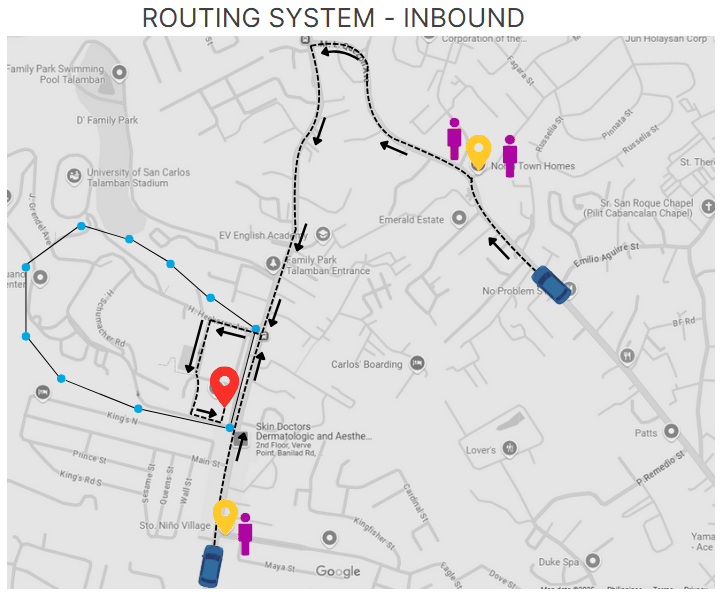
\includegraphics[width=0.54\textwidth]{images/Proximity zone inbound.png} % Adjust width as needed
    \caption{Estimated Proximity Zone for Inbound USC-TC Ride}
    \label{fig: Proximity zone inbound}
\end{figure}

\begin{figure}[htbp] % 'h' means "here" (suggested placement)
    \centering
    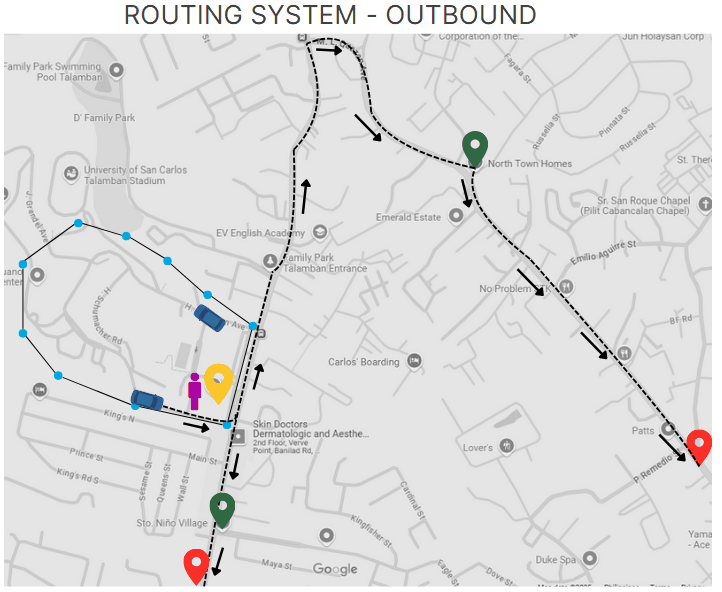
\includegraphics[width=0.54\textwidth]{images/Proximity zone outbound.png} % Adjust width as needed
    \caption{Estimated Proximity Zone for Outbound USC-TC Ride}
    \label{fig: Proximity zone outbound}
\end{figure}

\begin{figure}[htbp] % 'h' means "here" (suggested placement)
    \centering
    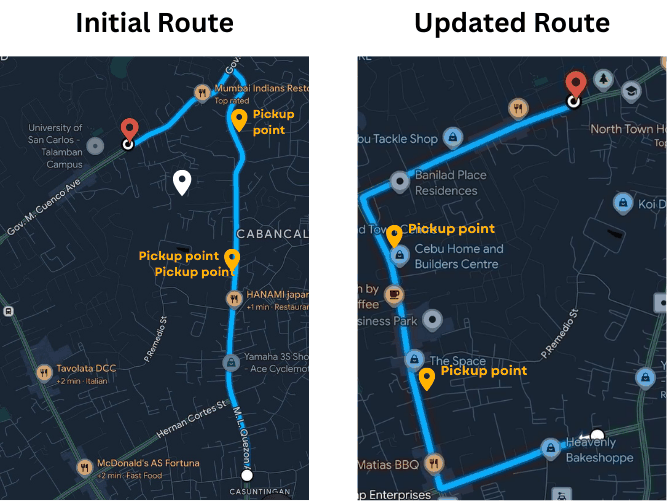
\includegraphics[width=0.92\textwidth]{images/Routing Figure.png} % Adjust width as needed
    \caption{Routing Example}
    \label{fig:routing}
\end{figure}

A core feature of the routing system is its ability to detect deviations from the suggested route and automatically generate a new optimized path in real time. A routing example is shown in Figure~\ref{fig:routing}. This applies to both inbound and outbound trips. For inbound travel to USC Talamban Campus, the application initially calculates an optimized route from the student driver’s current location to the campus, incorporating predefined pickup points situated along major roads and bus stops. As the driver begins the journey, the system constantly monitors their GPS position. If the driver takes a turn or route that deviates from the suggested path, the Google Routes API (through the \texttt{computeRouteAsia} Cloud Function) is called to recalculate a new route to the original destination—USC Talamban Campus—while still attempting to pass through as many nearby pickup points as possible. This dynamic rerouting, demonstrated in Figures~\ref{fig: generated route} and~\ref{fig: recalculated route} ensures minimal disruption to the ride-matching process, while allowing the driver to navigate based on real-time road conditions or personal preferences.

\begin{figure}[htbp] % 'h' means "here" (suggested placement)
    \centering
    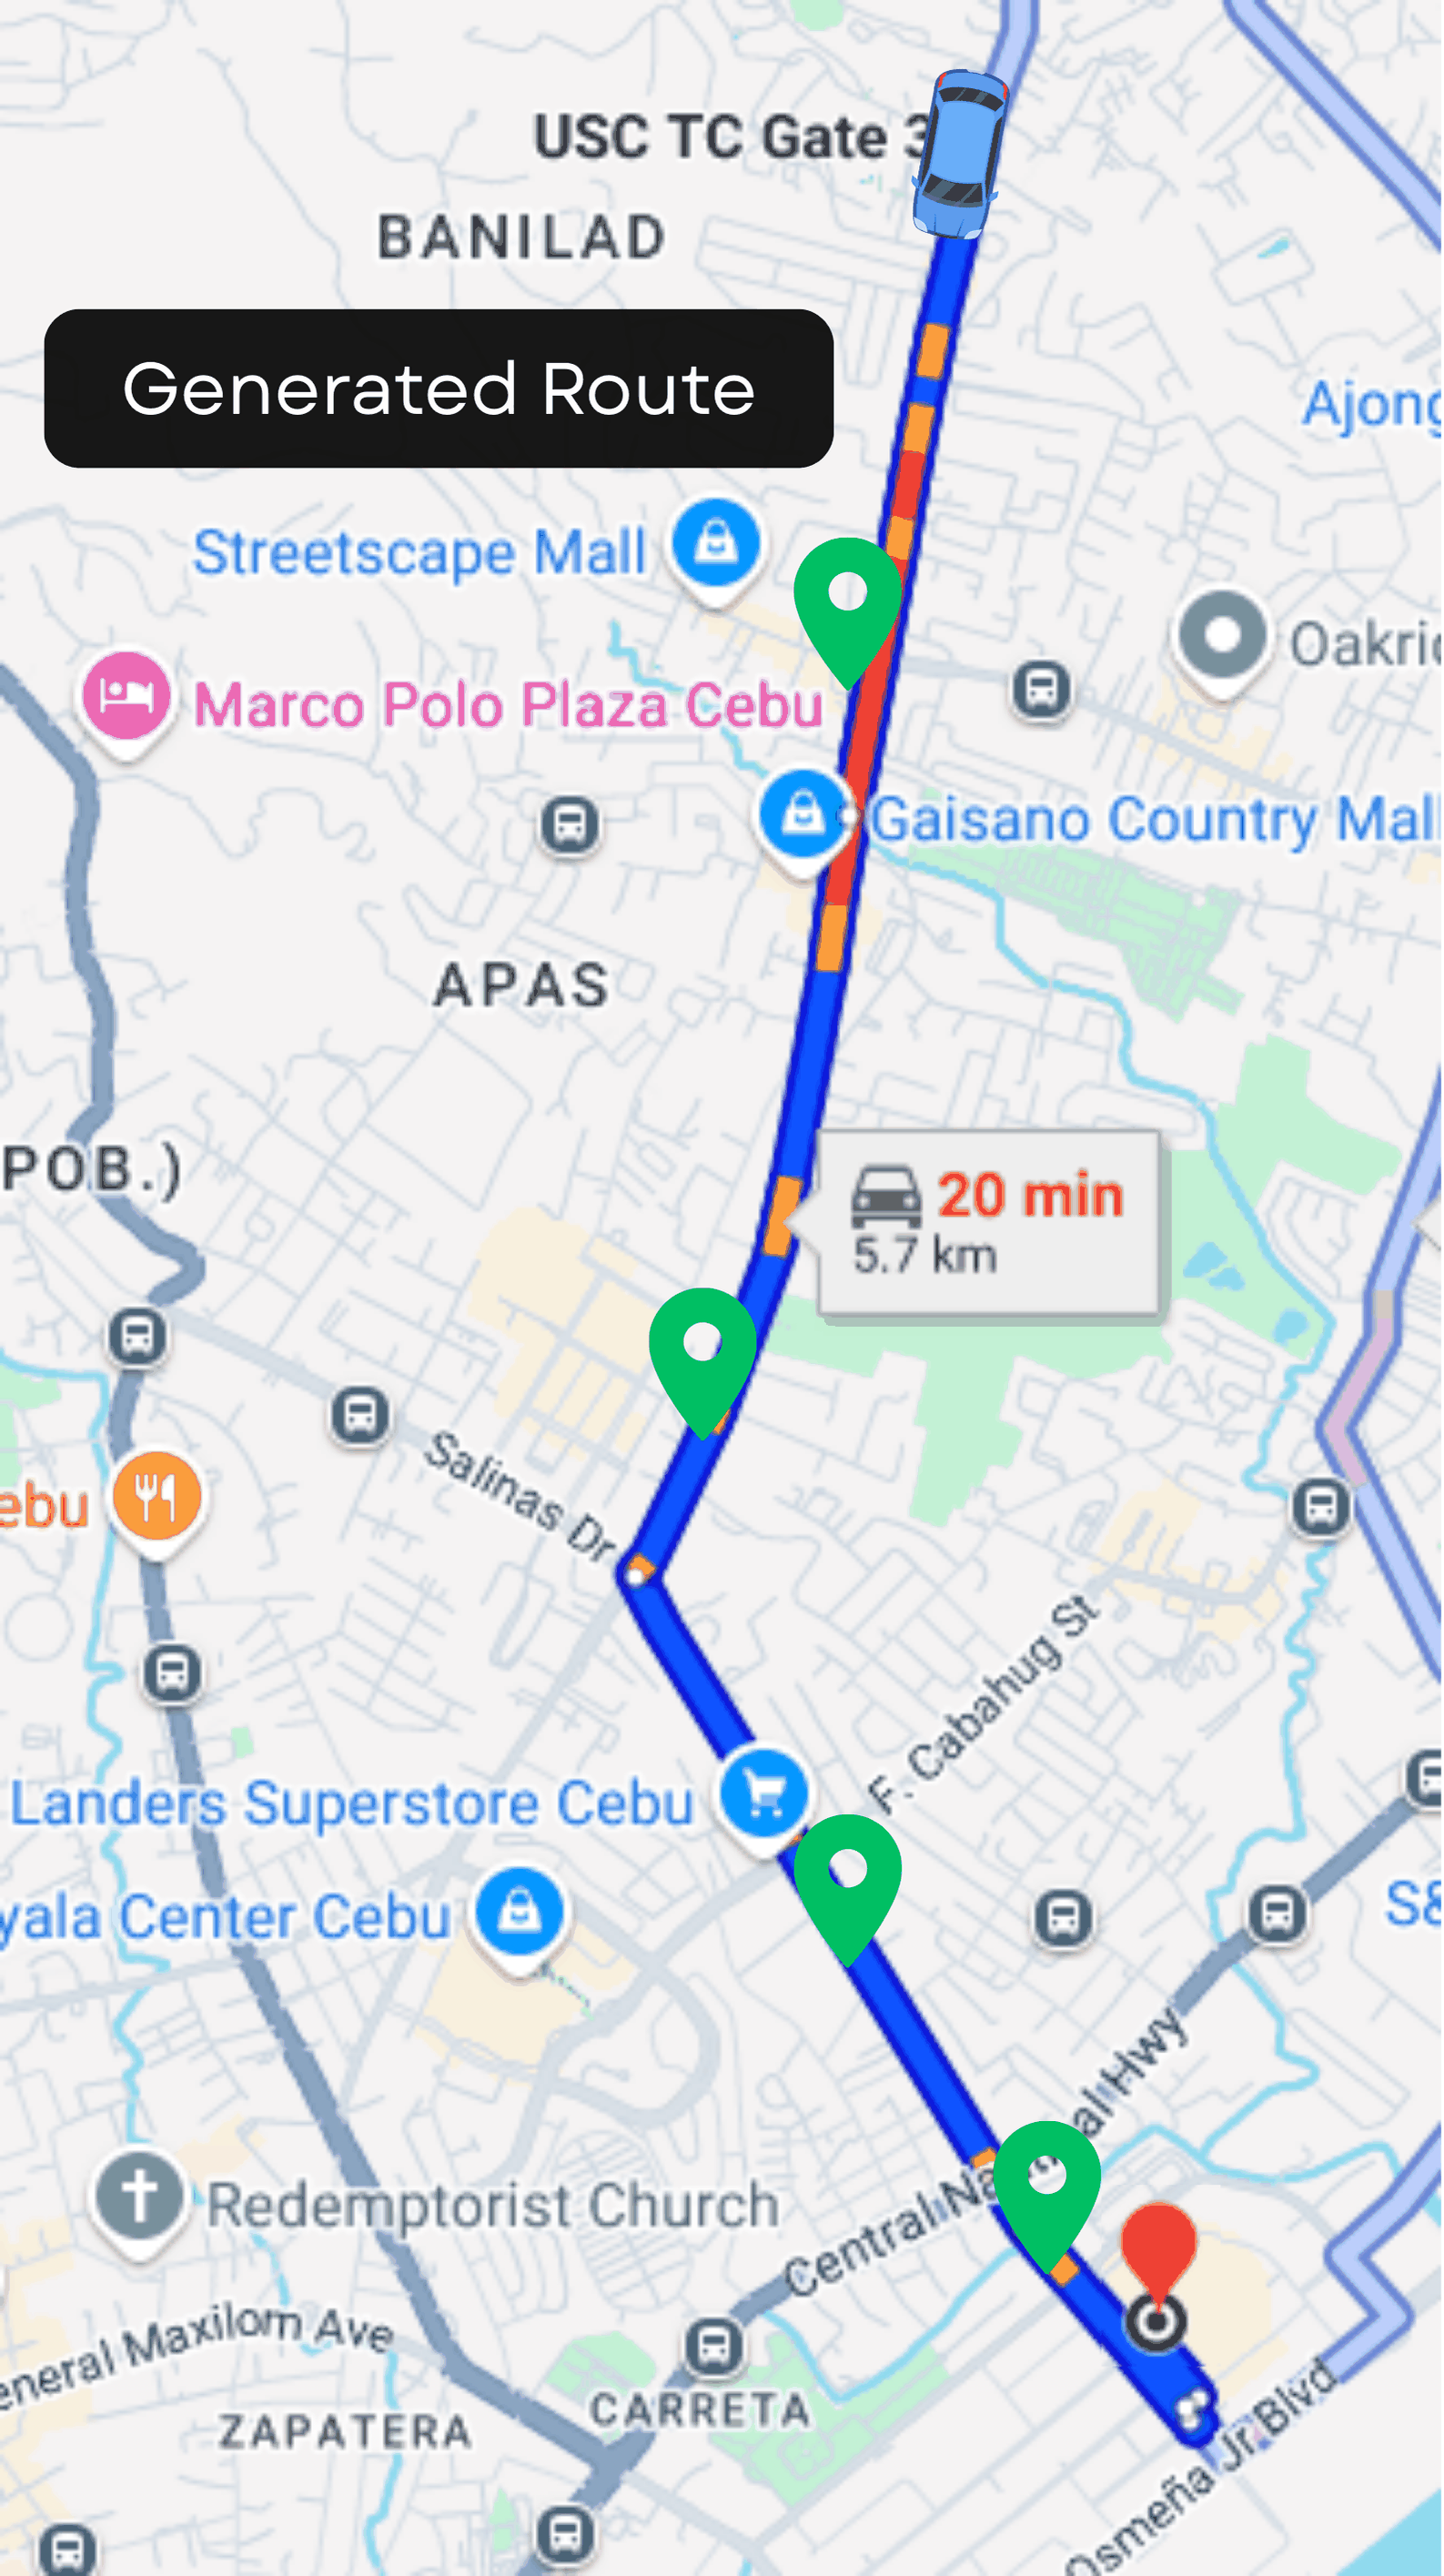
\includegraphics[width=0.48\textwidth]{images/outbound route.png} % Adjust width as needed
    \caption{Sample Optimized Route (Outbound TC)}
    \label{fig: generated route}
\end{figure}

\begin{figure}[htbp] % 'h' means "here" (suggested placement)
    \centering
    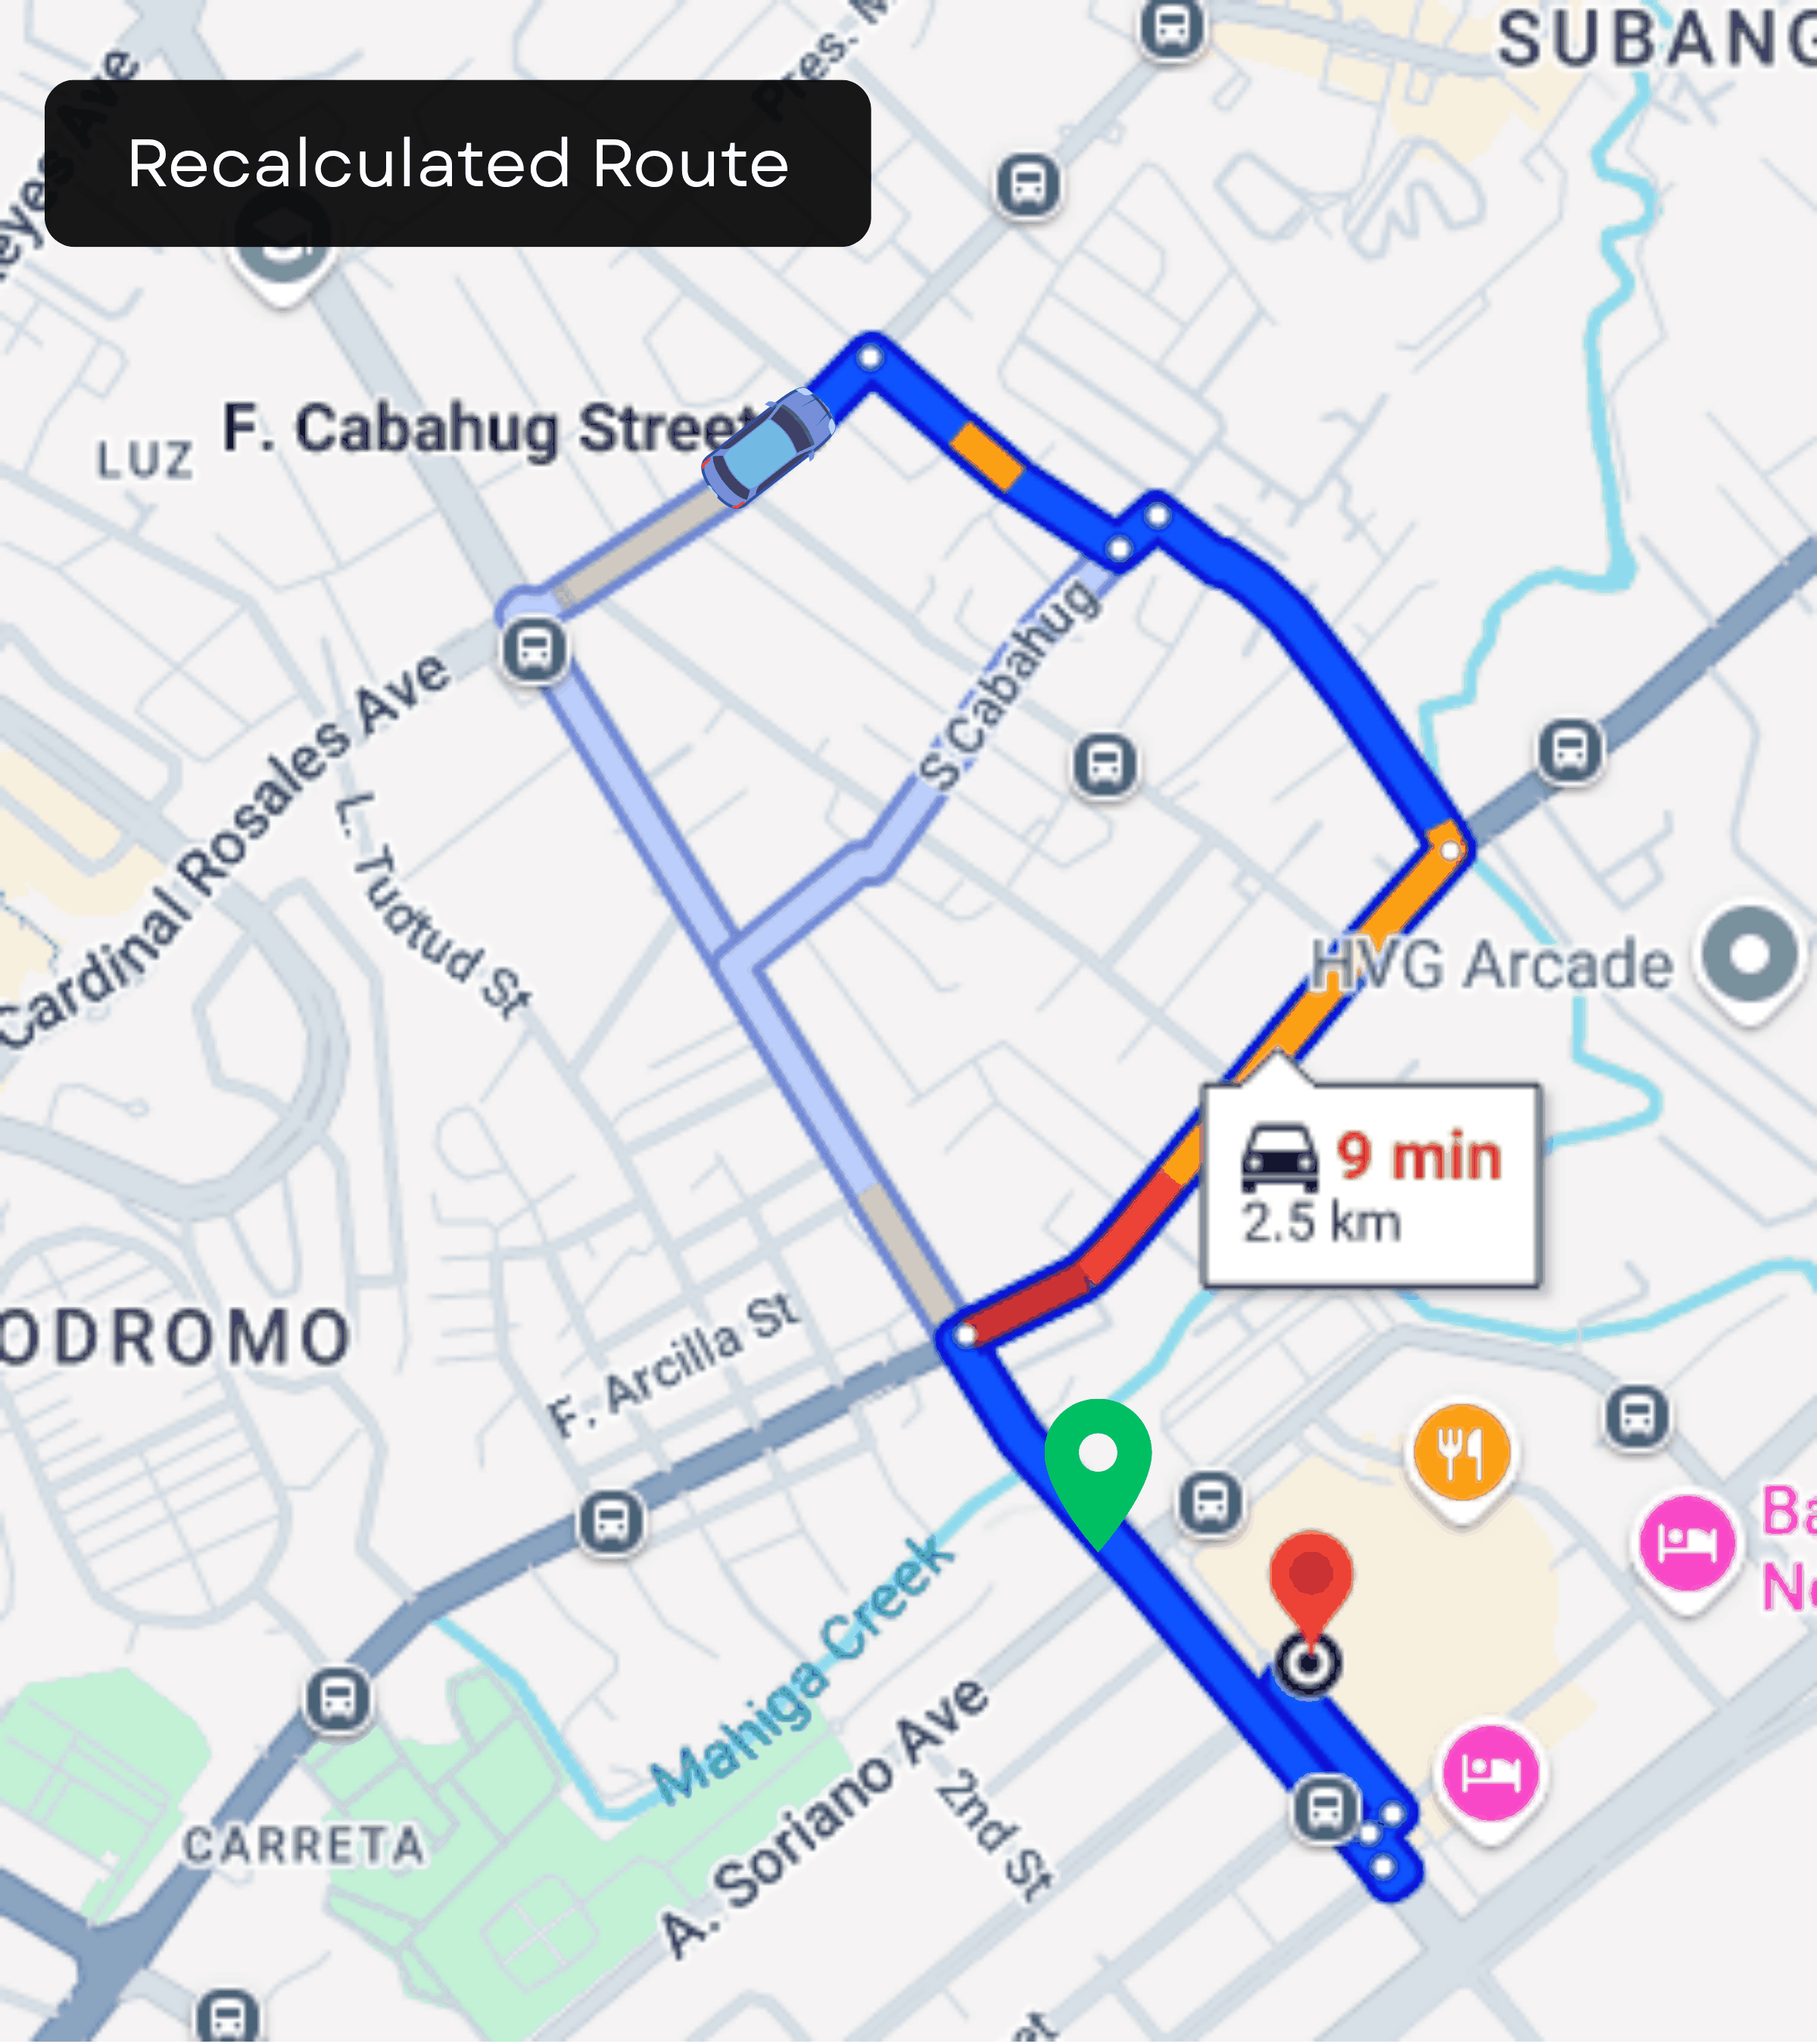
\includegraphics[width=0.48\textwidth]{images/recalculated outbound.png} % Adjust width as needed
    \caption{Sample Recalculated Route after Driver Deviates (Outbound TC)}
    \label{fig: recalculated route}
\end{figure}


\section{Ride-matching Algorithm}
\label{sec:matching}
\begin{figure}[htbp] % 'h' means "here" (suggested placement)
    \centering
    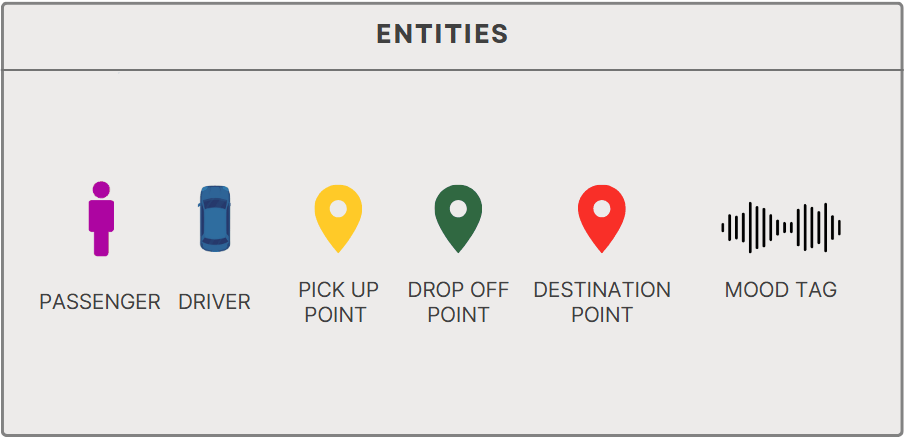
\includegraphics[width=0.54\textwidth]{images/Entities.png} % Adjust width as needed
    \caption{Ride-matching Entities}
    \label{fig: entities}
\end{figure}
As shown in Figure~\ref{fig: entities} the ride-matching algorithm operates based on the interaction of the following entities:
\begin{itemize}
    \item Pickup/Drop-Off Point: All passenger interactions are anchored to fixed pickup/drop-off points.
    \item Destination Point: The target location of the trip (e.g., USC Talamban Campus or end point of the driver). 
    \item Driver: Students who offer rides. Each driver follows an optimized route.
    \item Passenger: Students requesting transport
\end{itemize}

These entities collectively influence the algorithm’s decision-making—who gets matched, when, and where—based on location data, proximity zones, and real-time route optimization.

\vspace{1em}
\subsection{Inbound Ride-Matching System Logic}
\indent For inbound trips heading toward USC Talamban Campus, the system applies a structured ride-matching flow that prioritizes driver control, optimized routing, and context-aware notifications. 
Once a student driver marks themselves available, the application immediately generates an optimized route using the Google Routes API through a Cloud Function. Along this route, the system displays predefined pickup points—locations where passengers have submitted requests and are actively waiting. A sample route be seen in Figure~\ref{fig: sample inbound ride matching}.

\begin{figure}[htbp] % 'h' means "here" (suggested placement)
    \centering
    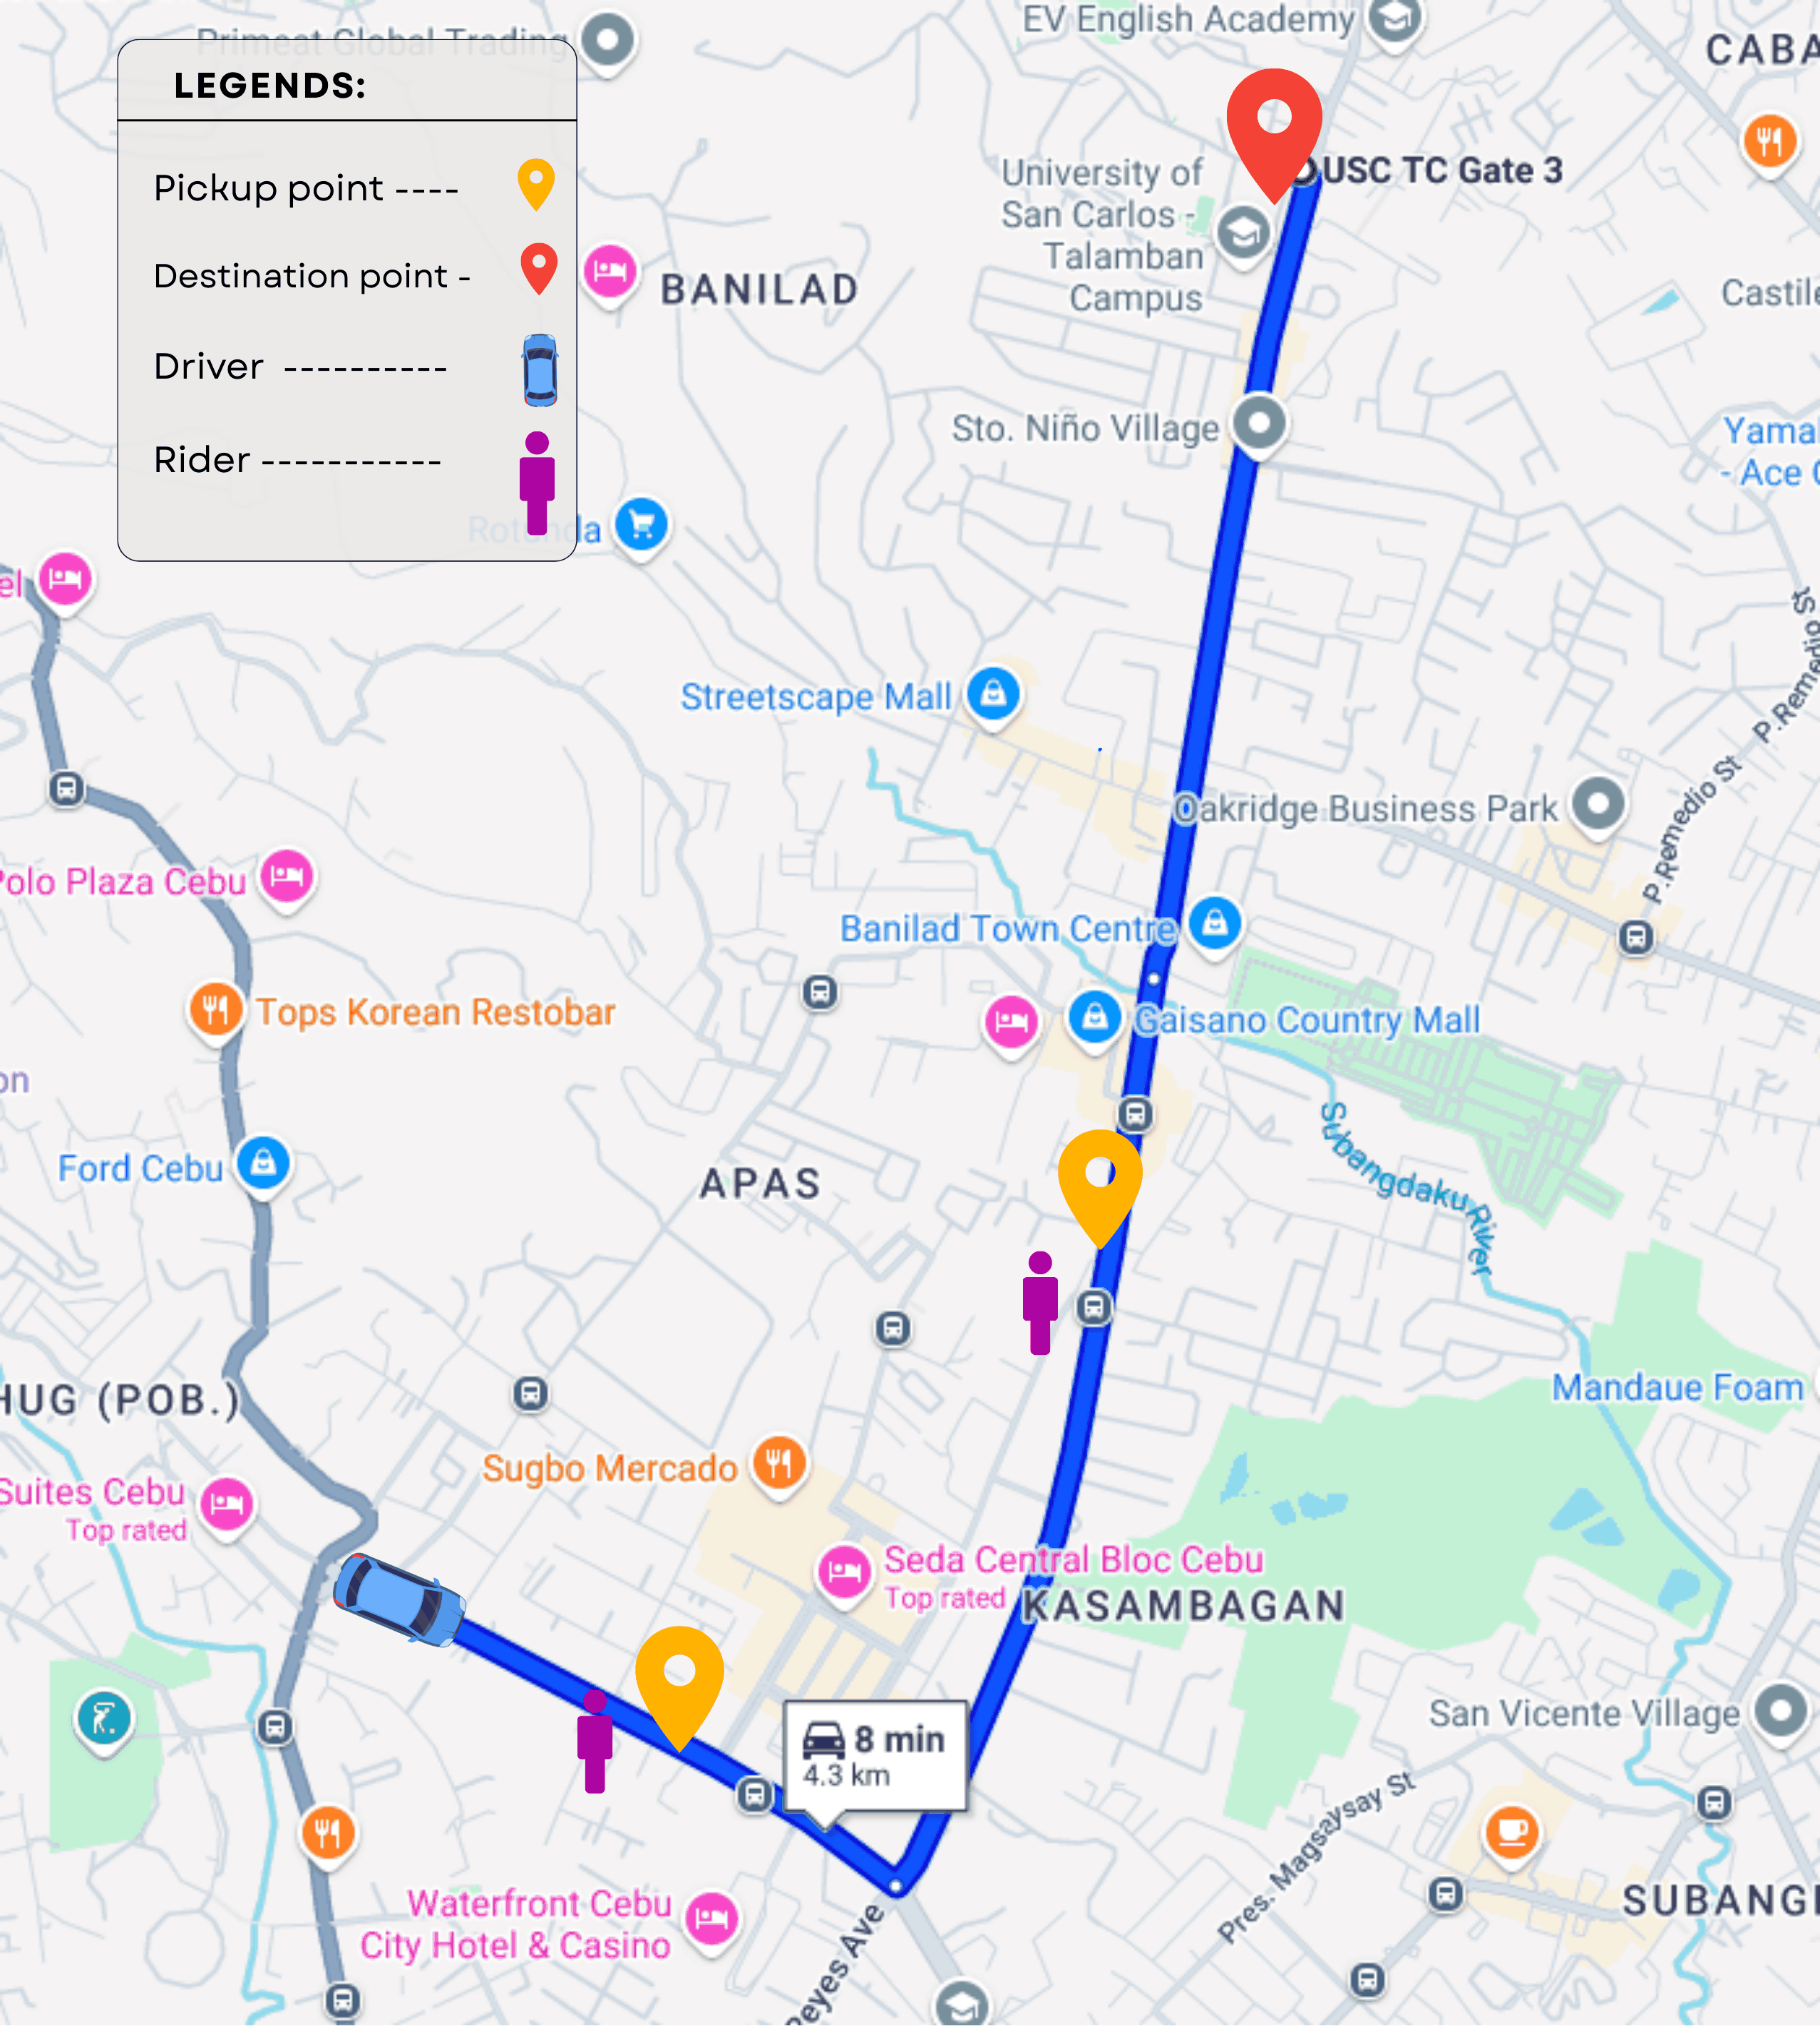
\includegraphics[width=0.6\textwidth]{images/RIDE MATCHING FIGURES.png} % Adjust width as needed
    \caption{Sample Inbound Ride-Matching System Logic}
    \label{fig: sample inbound ride matching}
\end{figure}

The driver interface presents requests associated with pickup points near the remaining route. Route proximity is a client-side display filter; it is not independently verified by the server when a request is accepted.

\begin{figure}[htbp] % 'h' means "here" (suggested placement)
    \centering
    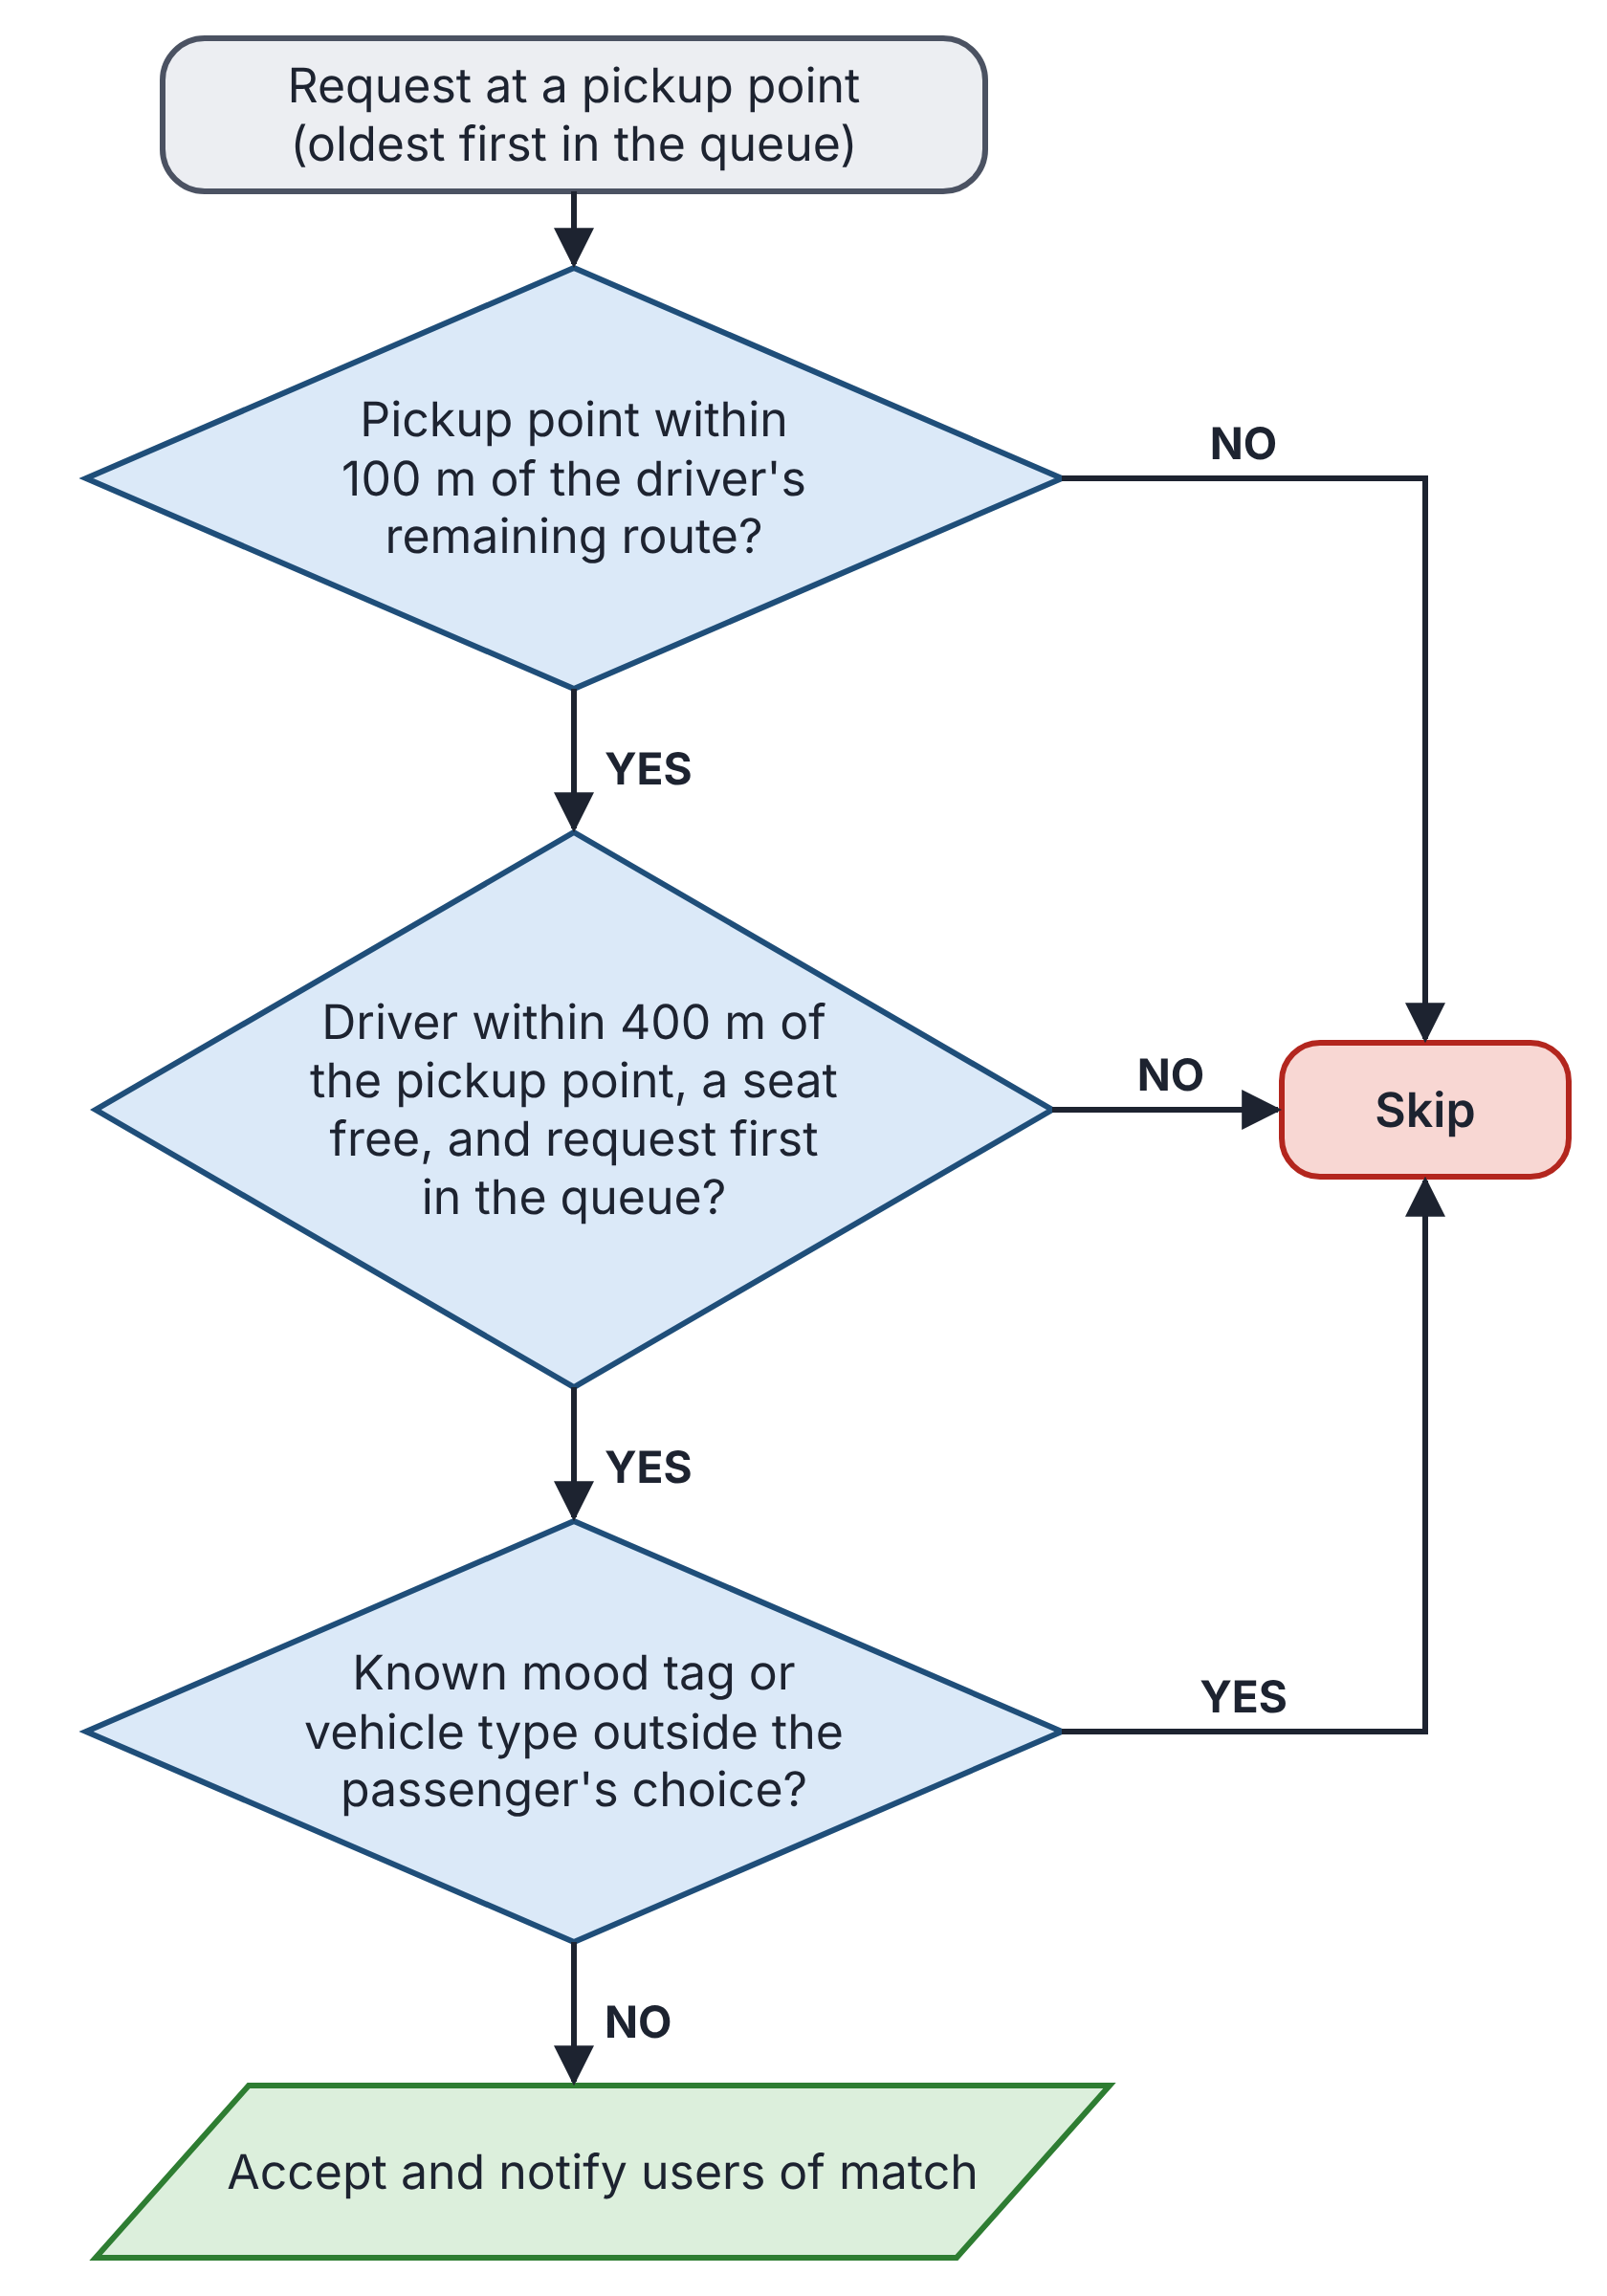
\includegraphics[width=0.6\textwidth]{images/Conditions.png} % Adjust width as needed
    \caption{Matching Conditions Logic}
    \label{fig: matching conditions}
\end{figure}

On the driver's screen, route alignment uses the route-match distance from the relevant ride point to the remaining route (Table~\ref{tab:rules-by-setting}). Requests at the same queue point and direction are ordered by creation time. On acceptance, the \texttt{matchRide} Cloud Function checks that the request is pending, the driver is available and approved, the trip direction and position relative to the geofence agree, and a seat remains. The driver's straight-line distance from the pickup must be no more than the acceptance distance of the trip's direction (Table~\ref{tab:rules-by-setting}). The function also checks queue order and vehicle preference before updating the request and capacity in a transaction. An unknown vehicle type is treated as compatible. The server does not independently recheck the route-proximity filter because it does not have the route polyline.

The distances of these checks depend on the setting. The design setting is real-life commuting, which is what the system was designed for. The controlled setting was used only for testing and demonstration, and it uses a smaller geofence and shorter distances. The values of the design setting were used mostly in the alpha testing, the beta testing, and the dry run before the UAT, and the values of the controlled setting were used in the UAT. Table~\ref{tab:rules-by-setting} gives both.

\begin{table}[htbp]
    \centering
    \caption{Distance and Area Rules by Setting}
    \label{tab:rules-by-setting}
    \small
    \renewcommand{\arraystretch}{1.25}
    \begin{tabular}{|>{\raggedright\arraybackslash}p{0.27\textwidth}|>{\raggedright\arraybackslash}p{0.30\textwidth}|>{\raggedright\arraybackslash}p{0.30\textwidth}|}
        \hline
        \textbf{Rule} & \textbf{Design setting (real-life commuting)} & \textbf{Controlled setting (testing and demonstration)} \\
        \hline
        Geofence area & A polygon around the USC-TC campus & A smaller polygon around the Bunzel building \\
        \hline
        Trip direction & Inside the geofence: outbound. Outside: inbound. & Inside the Bunzel geofence: outbound. Outside: inbound. \\
        \hline
        Inbound request distance (passenger to the selected pickup point) & Within 100 m & Within 20 m \\
        \hline
        Outbound request (passenger) & Inside the campus geofence and within 100 m of Bunzel & Inside the Bunzel geofence \\
        \hline
        Route-match distance (point to the driver's route) & Within 100 m & Within 30 m \\
        \hline
        Acceptance distance, inbound (driver to the pickup point) & Within 400 m & Within 100 m \\
        \hline
        Acceptance distance, outbound (driver to the pickup point) & Within 400 m & Within 400 m \\
        \hline
        Pickup confirmation & No distance check after acceptance & No distance check after acceptance \\
        \hline
        Inbound ride completion & Inside the campus geofence or within 150 m of Bunzel & Inside the Bunzel geofence or within 150 m of Bunzel \\
        \hline
        Outbound drop-off confirmation & Within 150 m of the passenger's destination & Within 30 m of the passenger's destination \\
        \hline
    \end{tabular}
\end{table}

Two further limits keep the interaction safe and relevant. An inbound passenger can only request a pickup point that is within the inbound request distance of their position. A driver is shown a request only when its pickup point is within the route-match distance of the remaining route, and can accept it only when the driver is within the acceptance distance of the pickup point and the passengers on board are below the vehicle's capacity. When a driver's position changes so that a waiting request becomes eligible under these checks, a Cloud Function uses the same server-side eligibility check as acceptance and sends a push notification, so the driver does not have to keep the screen open. To limit distraction, an inbound driver is prompted only when a passenger is 60 to 100~m ahead; the original design used a window of 300 to 400~m. When the match is accepted, the server also copies each side's display name and rating, and the driver's vehicle type and plate number, onto the request so that the two riders can recognize each other.

This logic is consistent with optimization practices found in ride-hailing literature, where user fairness and system-level route efficiency are jointly considered to balance service quality and operational practicality \cite{cao2021optimization}. Additionally, minimizing cognitive load on drivers through controlled notifications aligns with research showing that poorly timed prompts can contribute to distracted driving and reduce overall safety—particularly among younger, less experienced drivers such as university students \cite{xing2024understanding,oviedo2018young}. By showing a driver only requests that are on the route, close enough to accept, and within capacity, and by notifying only when a request becomes eligible, the system limits unnecessary prompts while maintaining real-time responsiveness in a multi-user environment.

\vspace{1em}

\begin{figure}[htbp] % 'h' means "here" (suggested placement)
    \centering
    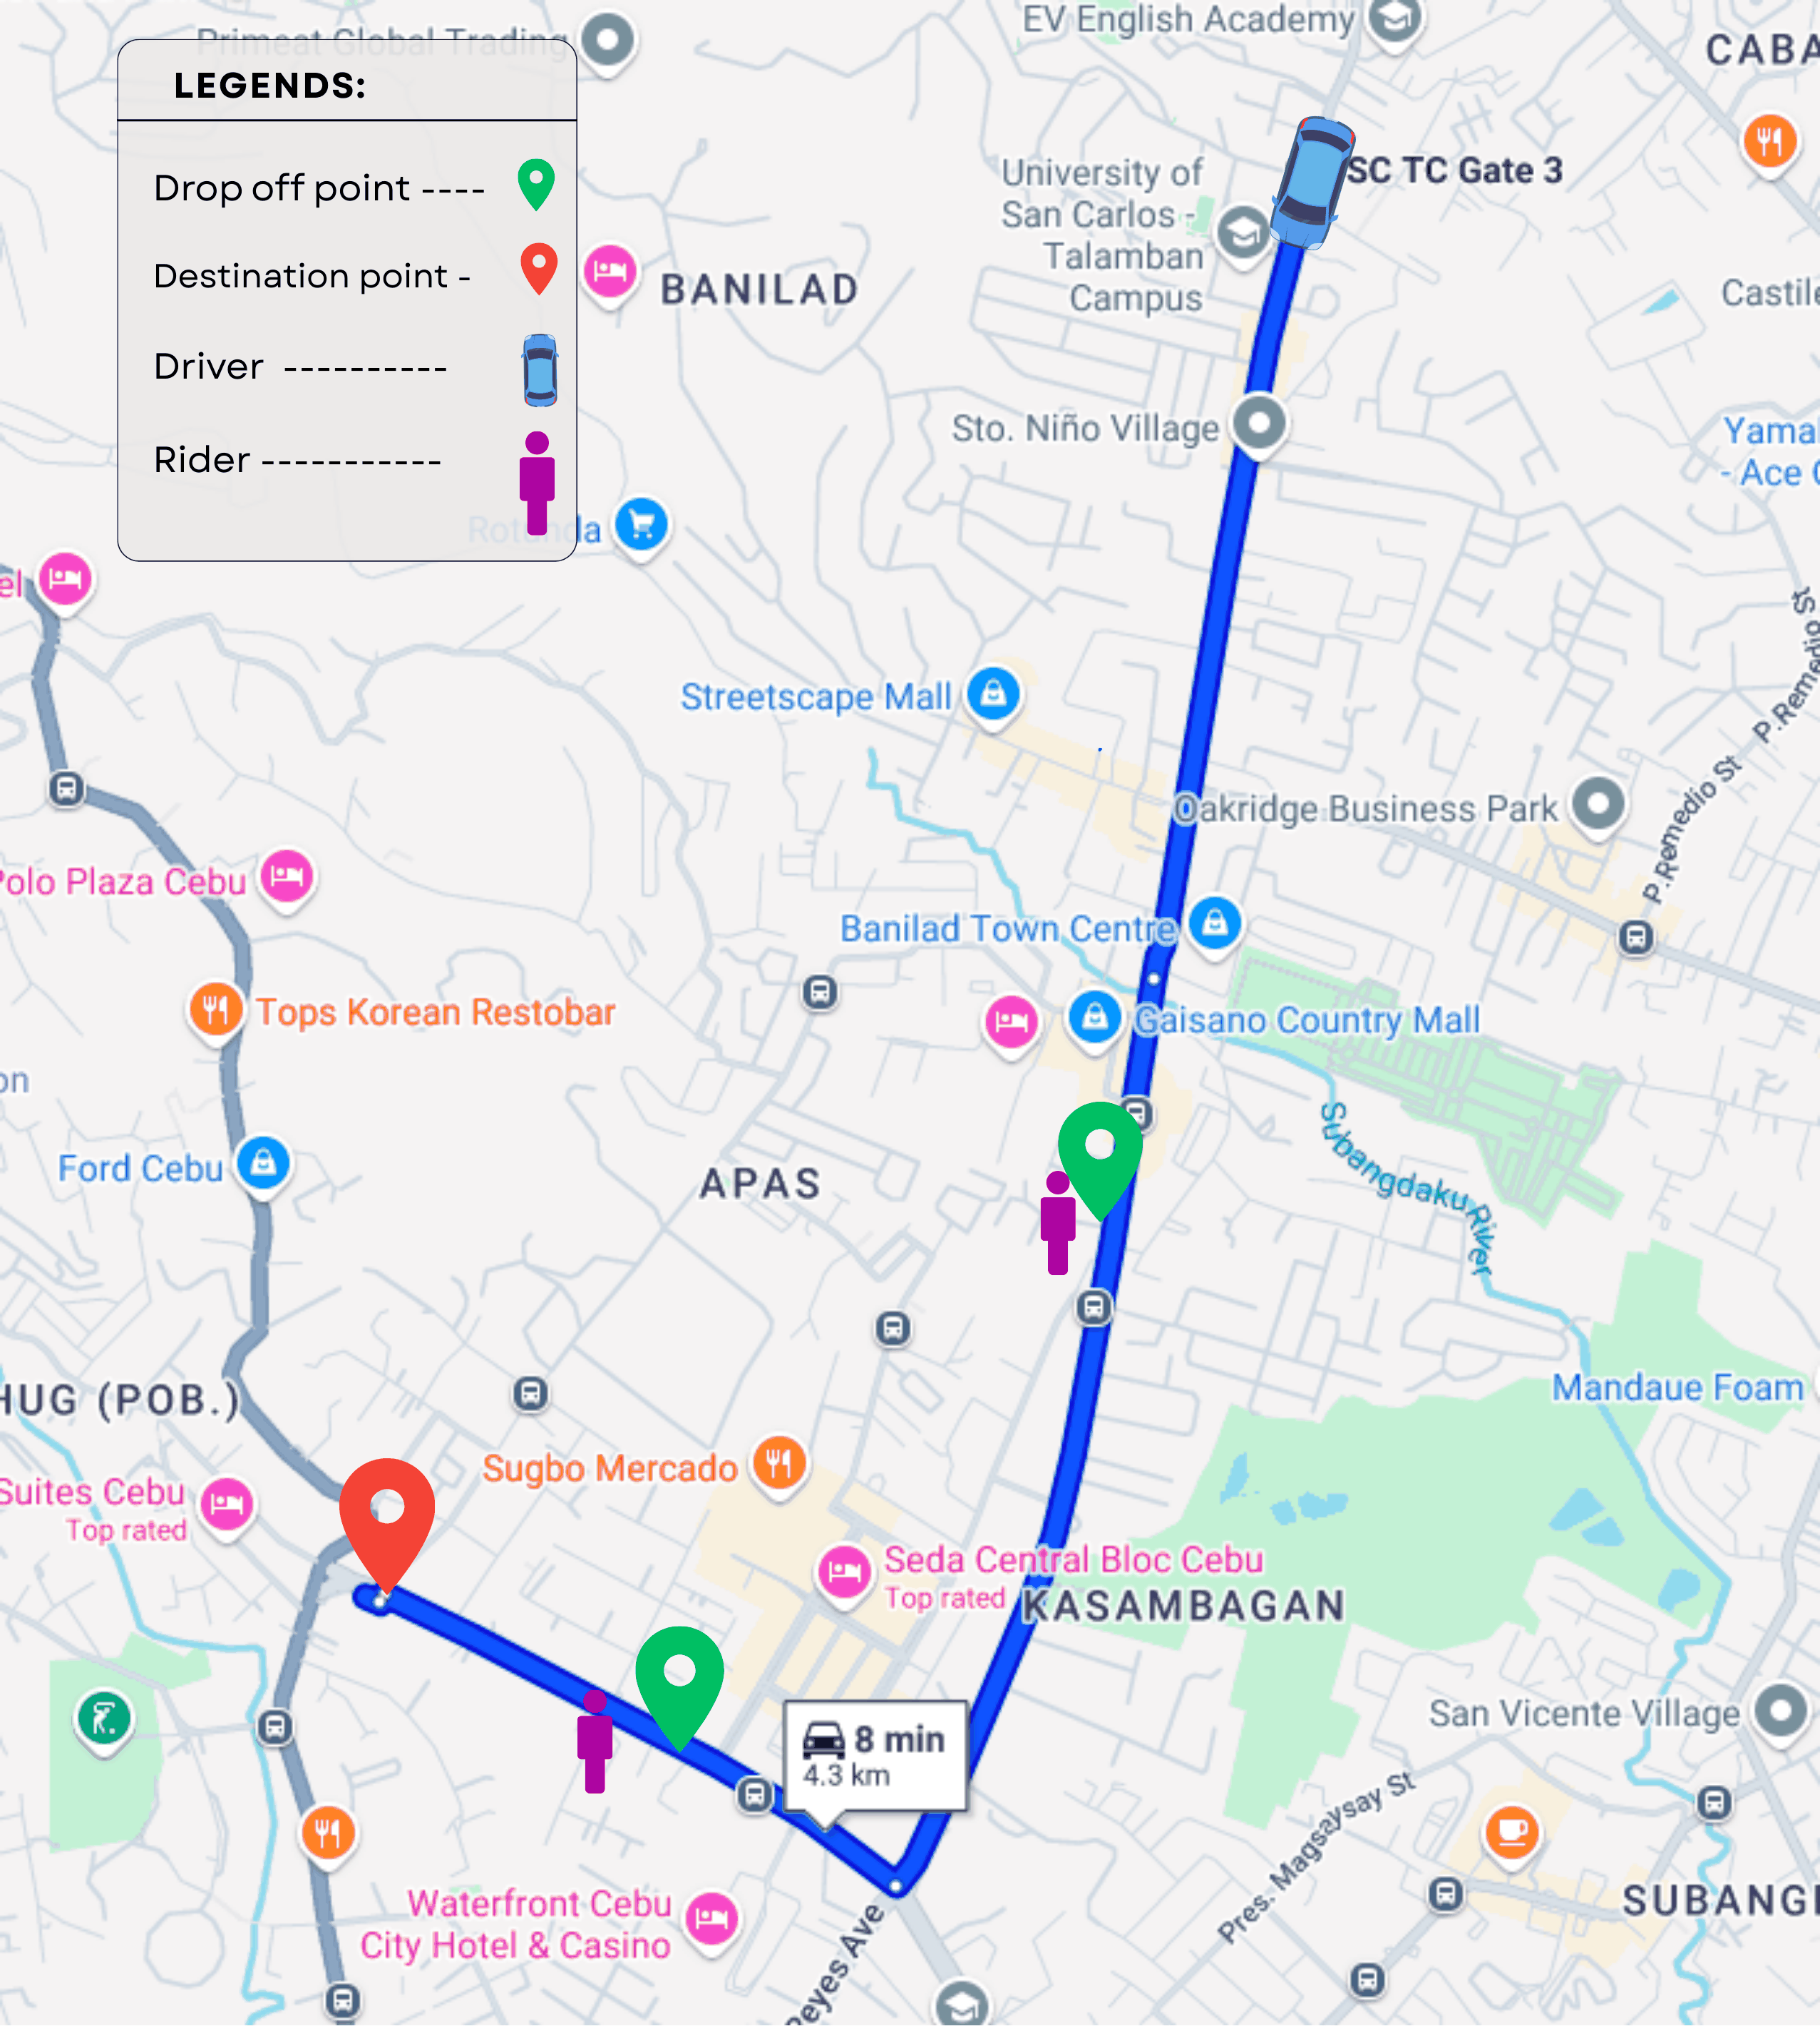
\includegraphics[width=0.6\textwidth]{images/OUTBOUND.png} % Adjust width as needed
    \caption{Sample Outbound Ride-Matching System Logic}
    \label{fig: sample outbound ride matching}
\end{figure}

\subsection{Outbound Ride-Matching System Logic} 
\indent For outbound rides, the journey begins at the Bunzel Lobby dispatch point inside the USC Talamban Campus. In this scenario, the driver first selects their intended end destination—typically near their home or an area they plan to pass through after school—either by typing it in a search field or by dropping a pin on the map. An example scenario is shown in Figure~\ref{fig: sample outbound ride matching}.

Once the driver has chosen a destination, the algorithm generates an optimized route using the Google Routes API, mapping the path from Talamban Campus to the selected endpoint. Along this route, the system automatically scans for predefined drop-off points that fall within or closely align with the optimized path.

The application then presents the list of eligible drop-off points to the driver, each showing how many passengers have active requests to be dropped off at that specific location. This gives the driver the ability to assess demand along their chosen path.

The driver then accepts passenger requests for specific drop-off points that they are willing to accommodate. Once confirmed, the system updates the ride plan, grouping passengers by shared drop-off locations, while continuously monitoring route progress and rerouting if necessary due to detours or road conditions.

A passenger's client cannot tell which drivers are available or where they are heading, so when a request at a drop-off point is not accepted, the alternative drop-off points offered to the passenger are ranked on the server by the \texttt{suggestAlternativeDropOffs} function. It reads the destinations of the currently available outbound drivers and ranks the other approved points by how close they are to those destinations, so that the passenger sees, for example, ``2 drivers heading this way''. The function only reads data; it never decides whether a request can be accepted, which remains the job of \texttt{matchRide}. A passenger who needs to leave before the final drop-off can request an early drop-off, and the driver is notified.

The outbound ride-matching system at USC Talamban Campus leverages advanced commute management strategies, similar to those employed by platforms like CommuteHub from RideAmigos [1]. This system ensures efficient ride sharing by matching passengers with drivers whose routes include their drop-off points, aligning with best practices in transportation demand management (TDM) that emphasize streamlined trip planning and coordination to reduce congestion and enhance user experience \cite{rideamigosHomepage,wsutdm}. By integrating personalized mobility options and optimizing drop-offs, the system provides drivers with control over their routes while minimizing detours \cite{rideamigosHomepage}.

% \uishot[width]{file-name-without-extension}{caption under the screen}
\providecommand{\uishot}[3][0.23\textwidth]{%
  \begin{minipage}[t]{#1}\centering
    \IfFileExists{images/ui/#2.png}%
      {\includegraphics[width=\linewidth]{images/ui/#2.png}}%
      {\fbox{\parbox[c][6.2cm][c]{\dimexpr\linewidth-2\fboxsep-2\fboxrule\relax}{\centering\footnotesize Screenshot pending:\\[2pt]\texttt{#2}}}}\\[3pt]
    {\footnotesize #3}
  \end{minipage}}

% \flowimg{width as a fraction of the text width}{flowchart file name without extension}
\providecommand{\flowimg}[2]{%
  \IfFileExists{images/#2.png}%
    {\includegraphics[width=#1\textwidth,height=0.80\textheight,keepaspectratio]{images/#2.png}}%
    {\fbox{\parbox[c][7cm][c]{0.8\textwidth}{\centering Flowchart pending:\\[2pt]\texttt{#2}}}}}

% \flowsplit{caption}{label}{chart name}: a compact swimlane flowchart (images/compact-flowcharts/<name>.png),
% set as one figure at full text width so that it fits on a single page.
\providecommand{\flowsplit}[3]{%
  \begin{figure}[htbp]\centering
    \includegraphics[width=\textwidth,height=0.82\textheight,keepaspectratio]{images/compact-flowcharts/#3.png}
    \caption{#1}\label{#2}
  \end{figure}}

\section{System Flow}
\label{sec:flow}
This section follows a user through the application. Each flow is shown twice: as a flowchart that gives the logic, and as screenshots of the actual application that show what the user sees at each step. The flowcharts use one colour per role (blue for steps shared by every user, green for drivers, yellow for passengers, and red for administrators). Circles name the screen a flow starts from or continues to.

\subsection{User Registration and Login}
A new user first sees a short welcome carousel, shown once per device (Figure~\ref{fig:ui-register}a). Registration then takes place in the steps of Figure~\ref{fig: registration}. The user chooses Passenger or Driver and enters a name, a USC email address ending in \texttt{@usc.edu.ph}, and a password (Figure~\ref{fig:ui-register}b). Drivers also declare their vehicle class, vehicle type, fuel type, and number of seats. The required documents are then uploaded (Figure~\ref{fig:ui-register}c): the USC School ID and Study Load for every user, plus the driver's license, OR/CR, and campus Motor Vehicle Pass for drivers, and proof of a second helmet for motorcycle drivers (Section~\ref{sec:safety}). Before submitting, the user accepts the terms and the liability waiver. A verification link is sent to the email address, and an administrator reviews the documents before the account can be used. Until then, and if the registration is denied or the account is suspended, the user sees a status screen with the reason (Figure~\ref{fig:ui-register}d) instead of the application.

    \flowsplit{User Registration}{fig: registration}{Registration}

    \begin{figure}[htbp]
        \centering
        \uishot{reg-welcome}{(a) Welcome}\hfill
        \uishot{reg-account}{(b) Create account}\hfill
        \uishot{reg-documents}{(c) Documents}\hfill
        \uishot{reg-pending}{(d) Awaiting approval}
        \caption{Screens of the registration flow}
        \label{fig:ui-register}
    \end{figure}

Login is shown in Figure~\ref{fig: login}. The user signs in with the USC email and password (Figure~\ref{fig:ui-login}a). If the email has not been verified, the application sends the verification link again and signs the user out. If the account is not approved, the status screen is shown. Approved administrators go to the Admin Menu. Everyone else arrives at the Home screen (Figure~\ref{fig:ui-login}b), which has four tabs (Home, Rides, Chats, and Profile). A first-time user is offered a short tour that can be skipped. A driver account has a mode switch on Home that chooses between Driver and Passenger (Figure~\ref{fig:ui-login}c); a passenger account always uses Passenger mode.

    \flowsplit{User Login}{fig: login}{Login}

    \begin{figure}[htbp]
        \centering
        \uishot[0.3\textwidth]{login}{(a) Login}\hfill
        \uishot[0.3\textwidth]{home-passenger}{(b) Home (passenger mode)}\hfill
        \uishot[0.3\textwidth]{home-driver}{(c) Home (driver mode)}
        \caption{Screens of the login flow}
        \label{fig:ui-login}
    \end{figure}

\subsection{Driver's Perspective}
\label{sec:flow-driver}
Figure~\ref{fig:driver menu} shows the user flow for the Driver Menu. The driver sets the rideshare details, which are the number of seats on offer, up to the capacity of the registered vehicle (Figure~\ref{fig:ui-driver-menu}a). Each driver's vehicle category and fuel type are declared in their profile, since the Ride Token calculation depends on them (Section~\ref{sec:tokens}). The driver then taps \emph{Confirm and check my location}. The application reads the driver's GPS position and asks the server to classify it against the campus geofence (Section~\ref{sec:routing}); if the server cannot be reached, the app uses its own copy of the geofence. A driver inside USC-TC is offered an outbound trip, and a driver outside it an inbound trip (Figure~\ref{fig:ui-driver-menu}b and c).

    \flowsplit{Driver Menu}{fig:driver menu}{Driver Menu}

    \begin{figure}[htbp]
        \centering
        \uishot[0.3\textwidth]{driver-details}{(a) Rideshare details}\hfill
        \uishot[0.3\textwidth]{driver-direction-outbound}{(b) Inside USC-TC: outbound}\hfill
        \uishot[0.3\textwidth]{driver-direction-inbound}{(c) Outside USC-TC: inbound}
        \caption{Screens of the Driver Menu}
        \label{fig:ui-driver-menu}
    \end{figure}

\paragraph{Inbound USC-TC} Figures~\ref{fig: Driver Inbound} and~\ref{fig: Driver Inbound 2} show the process a student driver follows when offering rides to USC-TC. The application draws a route from the driver's location to the Bunzel Lobby (Figure~\ref{fig:ui-driver-inbound}a). When the driver switches \emph{Available} on, the application saves the driver's availability, begins sharing the driver's location, and, for cars, starts mood detection (Section~\ref{sec:ai}). Requests whose pickup point lies within the route-match distance of the route are listed, oldest first at each pickup point, and drawn on the map (Figure~\ref{fig:ui-driver-inbound}b). The driver accepts a request by tapping \emph{Accept}, or turns on \emph{Auto-accept}, in which case the application accepts the oldest eligible request itself. In both cases the server repeats the checks of Section~\ref{sec:matching} before the request is accepted. After an acceptance, the seat count drops and the route is rebuilt through the accepted pickup points (Figure~\ref{fig:ui-driver-inbound}c). At each pickup point the driver taps \emph{Confirm pickup}; the first confirmation starts the trip and live tracking for the passengers. If the driver leaves the route by 75~m or more, the route is recalculated automatically. During the trip, a passenger may ask for an early drop-off, which the driver confirms. A driver may cancel a passenger who has not yet been picked up, which frees the seat, or end the whole trip early, in which case the passengers on board are recorded as \emph{terminated early} and no Ride Tokens are earned. When every accepted passenger has been picked up, the driver taps \emph{Complete ride} (Figure~\ref{fig:ui-driver-inbound}d).

    \flowsplit{Driver Inbound to USC-TC (1 of 2): going available and accepting requests}{fig: Driver Inbound}{Driver Inbound 1}

    \flowsplit{Driver Inbound to USC-TC (2 of 2): the trip}{fig: Driver Inbound 2}{Driver Inbound 2}

    \begin{figure}[htbp]
        \centering
        \uishot{di-route}{(a) Route and Available switch}\hfill
        \uishot{di-requests}{(b) Pending requests}\hfill
        \uishot{di-accepted}{(c) Accepted pickups}\hfill
        \uishot{di-complete}{(d) Complete ride}
        \caption{Screens of the Driver Inbound flow}
        \label{fig:ui-driver-inbound}
    \end{figure}

\paragraph{Outbound USC-TC} In Figures~\ref{fig:Driver Outbound} and~\ref{fig:Driver Outbound 2}, the driver offers rides from the campus to various destinations (for example, homes or malls). The driver types a destination in the search box or drops a pin on the map (Figure~\ref{fig:ui-driver-outbound}a). The application saves the destination, draws the route from the Bunzel Lobby, and lists the approved drop-off points along that route, each with the number of passengers waiting to be dropped there (Figure~\ref{fig:ui-driver-outbound}b). After switching \emph{Available} on, the driver accepts the requests for the drop-off points they are willing to serve (Figure~\ref{fig:ui-driver-outbound}c), or uses \emph{Auto-accept}. The server checks that the driver is within 400~m of the Bunzel Lobby and applies the other conditions of Section~\ref{sec:matching}. Accepted passengers are grouped by drop-off point. At the Bunzel Lobby the driver confirms each pickup, which starts the trip. Along the route the driver confirms each drop-off when within the confirmation distance of its point (Table~\ref{tab:rules-by-setting}) (Figure~\ref{fig:ui-driver-outbound}d); when the last passenger is dropped off, the trip is complete. Early drop-offs, cancellations, and early termination work as in the inbound flow.

    \flowsplit{Driver Outbound from USC-TC (1 of 2): going available and accepting requests}{fig:Driver Outbound}{Driver Outbound 1}

    \flowsplit{Driver Outbound from USC-TC (2 of 2): the trip}{fig:Driver Outbound 2}{Driver Outbound 2}

    \begin{figure}[htbp]
        \centering
        \uishot{do-destination}{(a) Destination search}\hfill
        \uishot{do-dropoffs}{(b) Drop-off points on the route}\hfill
        \uishot{do-requests}{(c) Pending requests}\hfill
        \uishot{do-confirm}{(d) Confirm drop-off}
        \caption{Screens of the Driver Outbound flow}
        \label{fig:ui-driver-outbound}
    \end{figure}

\subsection{Passenger's Perspective}
\label{sec:flow-passenger}
Figure~\ref{fig: passenger menu} shows the user flow for the Passenger Menu. The application reads the passenger's GPS position and asks the server to classify it against the campus geofence, as for drivers. A passenger inside USC-TC is taken to the outbound screen and one outside it to the inbound screen. If location is off or not permitted, an error with a \emph{Retry} button is shown.

    \flowsplit{Passenger Menu}{fig: passenger menu}{Passenger Menu}

\paragraph{Inbound USC-TC} Figures~\ref{fig: Passenger Inbound} and~\ref{fig: Passenger Inbound 2} outline the passenger's journey to the campus. The application shows the approved pickup points near the passenger, each marked \emph{In range} or \emph{Too far} (Figure~\ref{fig:ui-pax-inbound}a). A request can only be made for a point within the inbound request distance of the passenger. The passenger then chooses which moods to accept and a vehicle preference, where \emph{Any} matches every driver (Figure~\ref{fig:ui-pax-inbound}b), and taps \emph{Request ride}. The server creates the request, sets its direction from the pickup point, and fixes the passenger's place in the first-in, first-out queue of that pickup point. The waiting screen reads \emph{Looking for a driver} (Figure~\ref{fig:ui-pax-inbound}c). If the passenger moves away from the pickup point by more than that distance while waiting, the request is cancelled automatically. After about two minutes without a match, the passenger may accept more moods or vehicle types; this edits the same request, so the queue place does not change (Section~\ref{sec:moodmatch}). When a driver accepts, the passenger is notified, can follow the driver's location on the map, and can chat with the driver (Figure~\ref{fig:ui-pax-inbound}d). If the driver cancels or ends the trip early, the passenger sees a notice and may request again. A passenger who needs to leave before the end can ask for an early drop-off, which the driver confirms.

    \flowsplit{Passenger Inbound to USC-TC (1 of 2): requesting a ride}{fig: Passenger Inbound}{Passenger Inbound 1}

    \flowsplit{Passenger Inbound to USC-TC (2 of 2): the trip}{fig: Passenger Inbound 2}{Passenger Inbound 2}

    \begin{figure}[htbp]
        \centering
        \uishot{pi-points}{(a) Pickup points}\hfill
        \uishot{pi-preferences}{(b) Mood and vehicle preference}\hfill
        \uishot{pi-waiting}{(c) Waiting for a driver}\hfill
        \uishot{pi-matched}{(d) Driver on the way}
        \caption{Screens of the Passenger Inbound flow}
        \label{fig:ui-pax-inbound}
    \end{figure}

\paragraph{Outbound USC-TC} Figures~\ref{fig: Passenger Outbound} and~\ref{fig: Passenger Outbound 2} detail how a passenger books a trip from the campus to an external destination. The passenger must be inside the geofence, and the Bunzel Lobby is the only pickup point (Table~\ref{tab:rules-by-setting}). The passenger opens the drop-off picker and selects one of the approved drop-off points (Figure~\ref{fig:ui-pax-outbound}a), sets the preferences as for inbound trips, and taps \emph{Request ride}. If no driver accepts, the passenger can try a different drop-off point; the alternatives are ranked by how many available drivers are heading that way (Figure~\ref{fig:ui-pax-outbound}b, Section~\ref{sec:matching}). Once a driver accepts, the passenger is notified (Figure~\ref{fig:ui-pax-outbound}c), is picked up at the Bunzel Lobby, and is dropped off at the chosen point.

    \flowsplit{Passenger Outbound from USC-TC (1 of 2): requesting a ride}{fig: Passenger Outbound}{Passenger Outbound 1}

    \flowsplit{Passenger Outbound from USC-TC (2 of 2): the trip}{fig: Passenger Outbound 2}{Passenger Outbound 2}

    \begin{figure}[htbp]
        \centering
        \uishot[0.3\textwidth]{po-picker}{(a) Drop-off picker}\hfill
        \uishot[0.3\textwidth]{po-different}{(b) Try a different drop-off point}\hfill
        \uishot[0.3\textwidth]{po-matched}{(c) Driver on the way}
        \caption{Screens of the Passenger Outbound flow}
        \label{fig:ui-pax-outbound}
    \end{figure}

\subsection{After the Ride}
\label{sec:flow-after}
Figures~\ref{fig:after-driver} and~\ref{fig:after-passenger} show what happens when a trip ends. For the driver, the application records the ride, and the server measures the route and calculates the Ride Tokens; the client sends only the trip identifier and never a distance or a fuel price (Section~\ref{sec:tokens}). The completion screen shows the award as pending administrator review (Figure~\ref{fig:ui-after}a). An administrator checks each claim with its per-passenger breakdown, and the result appears in the driver's Token History (Figure~\ref{fig:ui-after}b). Passengers see a completion screen with an optional rating of the driver, which can also be given later from Ride Records (Figure~\ref{fig:ui-after}c). The matched pair can keep chatting for a short time after the ride (Figure~\ref{fig:ui-after}d). Either user can report a problem, and an emergency button is available during a ride; pressing it notifies the administrators and records the user's name, role, and the time (Figure~\ref{fig:ui-after}e and f).

    \flowsplit{Driver After the Ride}{fig:after-driver}{Driver After}

    \flowsplit{Passenger After the Ride}{fig:after-passenger}{Passenger After}

    \begin{figure}[htbp]
        \centering
        \uishot[0.27\textwidth]{after-driver-complete}{(a) Driver completion screen}\hfill
        \uishot[0.27\textwidth]{after-token-history}{(b) Token History}\hfill
        \uishot[0.27\textwidth]{after-passenger-rating}{(c) Passenger rating}\\[6pt]
        \uishot[0.27\textwidth]{after-chat}{(d) Ride chat}\hfill
        \uishot[0.27\textwidth]{after-report}{(e) Report a problem}\hfill
        \uishot[0.27\textwidth]{after-emergency}{(f) Emergency button}
        \caption{Screens after and during a ride}
        \label{fig:ui-after}
    \end{figure}

\subsection{Admin}
\label{sec:flow-admin}
Figure~\ref{fig: admin menu} shows the Admin Menu. The administrator signs in with secure credentials, and the dashboard shows how many items are waiting for a decision (Figure~\ref{fig:ui-admin}a). From the dashboard, the administrator has access to the following sections:
\begin{itemize}
    \item Registrations: Admins view, approve, or deny registration requests, giving a reason when denying (Figure~\ref{fig:ui-admin}b). Student drivers must submit essential documents such as the driver's license, OR/CR, and proof of university enrollment, which admins verify before granting access. Admins can also suspend and reinstate accounts, reset access, or update user details based on flagged behavior or violations.
    \item Reports: Admins receive and review reports from passengers and drivers, flag critical issues, and take appropriate action. A separate list shows the emergency alerts that users have raised (Figure~\ref{fig:ui-admin}c).
    \item Token Claims: Admins review each Ride Token award together with the recorded distances and the per-passenger breakdown, and can recalculate it if needed (Figure~\ref{fig:ui-admin}d).
    \item Ride Logs: The system stores all completed ride data. Admins use these logs to review ride history, monitor matching behavior, and ensure compliance with guidelines.
    \item Ride Points: Admins maintain the approved pickup and drop-off points (Figure~\ref{fig:ui-admin}e).
    \item Fuel Price and Semester Period: Admins check or refresh the DOE fuel price and its sync status, and set the dates of the semester that applies the 300-token cap (Figure~\ref{fig:ui-admin}f).
\end{itemize}

    \flowsplit{Admin Menu}{fig: admin menu}{admin}

    \begin{figure}[htbp]
        \centering
        \uishot[0.27\textwidth]{admin-dashboard}{(a) Dashboard}\hfill
        \uishot[0.27\textwidth]{admin-registrations}{(b) Registrations}\hfill
        \uishot[0.27\textwidth]{admin-reports}{(c) Reports and alerts}\\[6pt]
        \uishot[0.27\textwidth]{admin-token-claim}{(d) Token claim}\hfill
        \uishot[0.27\textwidth]{admin-ride-points}{(e) Ride Points}\hfill
        \uishot[0.27\textwidth]{admin-fuel-price}{(f) Fuel Price}
        \caption{Screens of the Admin flow}
        \label{fig:ui-admin}
    \end{figure}

This flow ensures that a central authority maintains order, enforces safety protocols, and provides accountability within the USC student ridesharing ecosystem.

\section{Non-Monetary Incentive System}
\label{sec:tokens}
To encourage sustainable transportation among students, our ridesharing platform introduces a non-monetary incentive system that allows student drivers to earn %Community Extension Services (CES) 
CES Points based on their contributions to shared transportation. This system operates separately from traditional CES activities (e.g., donation drives, tree planting) by providing a passive and recurring method for student drivers to contribute to the university’s sustainability initiatives.

Since direct monetary equivalence (1 CES Point = ₱100) would make it too easy to reach the 3 CES-Point-per-semester cap, a tokenomics approach is implemented. This model adjusts the conversion rate by introducing Ride Tokens, which reflect fuel consumption and distance traveled.

Each ride earns Ride Tokens based on the fuel expenditure required to complete the shared trip. The formula ensures that both short-distance and long-distance drivers are fairly rewarded, while also maintaining a balance between multi-passenger and single-passenger trips (e.g., motorcycle passengers).

The system adheres to the university’s standard CES point-to-peso ratio, where 1 CES Point = PHP 100. However, due to the unique nature of ridesharing, we introduce a token-based reward system (Ride Tokens) that factors in fuel costs and ride-sharing efficiency while ensuring fairness and engagement over multiple semesters.

\begin{itemize}
    \item 100 Tokens = 100 Pesos = 1 CES Point
    \item 3 CES Points per semester cap = 300 Ride Tokens per semester
    \item Maximum of 18 CES Points over 3 academic years (2 semesters) = 1,800 Ride Tokens
\end{itemize}

Each driver earns tokens based on:
\begin{itemize}
    \item Fuel Consumption: Calculated based on vehicle fuel efficiency (km/L) and prevailing fuel prices.
    \item Distance Traveled: The total distance covered while transporting passengers.
    \item Ride Distribution Factor: A weighting system that accounts for multiple pickups in a single trip.
\end{itemize}

To calculate the Ride Tokens, two inputs are needed: the fuel price and the vehicle's fuel efficiency. Fuel prices are taken from the DOE's weekly Cebu City ``Common Price'' report for gasoline and diesel. When a weekly value is missing, the median of the reported retailer prices is used instead; the median was preferred over the mean because it is less affected by outlier station prices. The fuel price is not typed in by anyone: a scheduled Cloud Function checks the DOE Visayas pump-price page every day, downloads the newest weekly report, reads the Cebu City rows for gasoline (RON 91) and diesel, and stores the result in Firestore only when it is newer than what is already there. There is no built-in default price: if the page cannot be read, the last price that was read successfully is kept, the failure is recorded, and the administrators are notified so that a stale price is noticed. Administrators can also refresh the price manually. Fuel efficiency is standardized by the vehicle category the driver declares at registration (Table~\ref{tab:efficiency}), taken from published specifications. Drivers choose one of eleven categories, and an ambiguous case is resolved by checking the make and model against the OR/CR that was already collected. A conservative figure per category is used, so that drivers are not rewarded for fuel consumption they did not actually incur.

\begin{table}[htbp]
    \centering
    \caption{Fuel Efficiency by Declared Vehicle Category}
    \label{tab:efficiency}
    \small
    \renewcommand{\arraystretch}{1.2}
    \begin{tabular}{|l|c|l|c|}
        \hline
        \textbf{Category} & \textbf{km/L} & \textbf{Category} & \textbf{km/L} \\
        \hline
        Motorcycle (standard) & 50 & SUV (compact, e.g., Raize) & 22 \\
        Motorcycle (scooter) & 55 & SUV (mid, e.g., Fortuner) & 12 \\
        Sedan (compact, e.g., Vios) & 26 & Pickup (light, gasoline) & 15 \\
        Sedan (mid, e.g., Accord) & 16 & Pickup (heavy, diesel) & 18 \\
        Crossover (small) & 20 & Minivan/MPV & 18 \\
        Crossover (mid) & 14 & & \\
        \hline
    \end{tabular}
\end{table}

The calculation is done entirely on the server. After the trip, the \texttt{calculateRideTokens} Cloud Function reads the trip's rides, measures the route itself through the Google Routes API, reads the stored fuel price, and writes the award with a per-passenger breakdown; the app sends only a trip identifier. The distance is that of the optimal ordering of the trip's stops, not the path the driver actually took. This is deliberate: the driven path is not stored on the server, a driver cannot earn more by taking a longer way round, and the award can be reproduced later from the same stops. Each leg is rounded to the nearest 10~m before the tokens are allocated, so that the figures printed on the admin review screen can be checked by hand. The function is idempotent, so a retry returns the existing award instead of paying twice.

Each driver earns Ride Tokens based on the distance traveled and the number of passengers. To balance fuel expenditure with CES incentives, we introduce a conversion factor that adjusts the number of tokens awarded per peso spent on fuel.

The base formula is:
\begin{equation}
    \text{Ride Tokens} = \frac{\text{Fuel Cost per Trip}}{\text{Ride Token Regulator}}
\end{equation}
Where: 
\begin{itemize}
    \item Fuel cost per trip is determined using real-time diesel and gasoline prices. Fuel consumption/efficiency per vehicle is dependent on the vehicle type, which is declared upon registration.
        \begin{equation}
            x = \text{Fuel price (PHP/L)}
        \end{equation}
    
        \begin{equation}
            y = \text{average fuel efficiency (km/L)}
        \end{equation}
        
        \begin{equation}
            d = \text{distance traveled (km)}
        \end{equation}
        
        \begin{equation}
            \text{Fuel Cost per Trip} = x * (\frac{d}{\text{y}})
        \end{equation}

    \item The \textit{Ride Token Regulator}, \textbf{5}, ensures the system remains engaging over multiple semesters rather than being easily maxed out in a few weeks and balances token distribution.

    \item The final Ride Token value is rounded up to the nearest hundredth.

\end{itemize}

For each additional passenger, their ride token contribution is determined by:
\begin{equation}
    \label{eq:extra}
    \frac{\text{Passenger Distance from Destination}}{\text{Total Shared Distance - Passenger Distance from Destination}}
\end{equation}
Where: 
\begin{itemize}
    \item \textit{Passenger Distance from Destination} = Distance from the passenger’s pick-up/drop-off point to the final destination

    \item \textit{Total Shared Distance} = Total distance from the first passenger’s pick-up to the final destination
\end{itemize}

Only drivers receive Ride Tokens; passengers do not earn tokens. When passengers share the same pick-up point and the same destination, their contributions are split equally, which also avoids a zero denominator in the distance ratio above. Values are rounded up to the nearest hundredth, as stated earlier.

An early drop-off, in which a passenger leaves the vehicle before the final drop-off, earns a flat 1 Ride Token for each such passenger, whatever its length or location. The exception is the first passenger of an outbound trip: if that passenger leaves early, for example because the driver stopped just outside the confirmation radius of the drop-off point and the ride had to be ended as an early drop-off, the passenger is priced like a regular rider and the award is calculated from the distance actually driven to where the passenger got off. The distance is measured to the actual exit point and not to the requested drop-off point, so a driver cannot claim a full trip by ending a ride shortly after pickup. The first passenger is the one picked up earliest. On inbound trips every early drop-off earns the flat rate. An early passenger paid at the flat rate does not take part in the distance calculation above and does not change anyone else's share. This was chosen because an early passenger's exit point can be any GPS position: when it fell a few metres from another passenger's pick-up, the ratio in Equation~(\ref{eq:extra}) divided by a near-zero gap and produced values of 67 to 101 Ride Tokens for rides that burned only a few tokens' worth of fuel. A trip made only of early drop-offs needs no fuel price or vehicle efficiency. The flat rate is not tied to fuel, so very short early rides are paid more than the fuel formula would give, and long ones less; this trade-off is accepted.

The ceilings above are enforced on the server. The driver's running total cannot exceed 300 Ride Tokens in the current semester or 1,800 across the programme. A ride that would pass a ceiling still completes, but the award is cut to the amount that fits and the excess is forfeited, not carried over; the ledger keeps both the uncapped value and the reason for the cut so that the administrator can see what the trip was really worth. The semester is defined by the dates that the administrator sets on the Semester Period screen. Until those dates are set, only the 1,800 ceiling applies.

\vspace{1em}

To better understand the scheme, the following example scenarios are provided. They use a fuel price of PHP 52 per liter, the example price used in the original proposal, and a driver who declared the mid-size SUV category (12~km/L, Table~\ref{tab:efficiency}). The vehicle category matters: the same 11~km trip earns about 2.08 Ride Tokens for a scooter and 9.54 for this SUV, so reaching the semester cap takes between about 32 and 145 shared rides depending on the vehicle. Scenarios A to C show a single passenger and several pickups. Scenarios D to I cover the other cases of the scheme: the vehicle category, passengers who share a pickup point, early drop-offs, the first passenger of an outbound trip who leaves early, and the semester ceiling. Unless stated otherwise, they keep the same fuel price and the same SUV. The trips of about 11~km in Scenarios A to I illustrate the scheme over a longer commute, such as the routes the system can support beyond USC-TC; they were not made in the study. Scenarios J to M are \textbf{for the controlled setting and for demonstration only}. They use campus-length trips, like the rides of the controlled testing, with the distances between campus buildings: about 0.5~km from the RH Building to the Bunzel building, about 0.4~km from the Bunzel building to SAFAD, and about 0.1~km from the MR Hall to the chapel. Scenario M uses assumed pickup points along the 0.5~km trip. These four scenarios show how the scheme behaves in the controlled testing; they are not examples of the Ride Tokens earned in real-life commuting, which is the setting the scheme was designed for and is illustrated by Scenarios A to I.

\vspace{1em}
\noindent\textit{Scenario A: Long-Distance Carpooler (11 km one way)}
\begin{itemize}
    \item A Student Driver picks up Student Passenger A 11 km away from USC-TC.
    \item Their vehicle consumes 11/12 $\approx$ 0.92 L of fuel for the 11 km.
    \item At PHP 52 per liter, the fuel cost is about PHP 47.67 per trip.
    \item Applying the Ride Token Regulator:
    \[
    \frac{47.67}{5} \approx 9.54 \text{ Ride Tokens per trip}
    \]
    \item For both pickup and drop-off:
    \[
    9.54 \times 2 = 19.08 \text{ Tokens per day}
    \]
    \item To reach 3 CES Points (300 Tokens per semester cap):
    \[
    \frac{300}{9.54} \approx 32 \text{ shared rides}
    \]
\end{itemize}

\begin{table}[htbp]
    \centering
    \caption{Scenario A Calculation Summary}
    \label{tab:scenario-a}
    \small
    \setlength{\tabcolsep}{4pt}
    \renewcommand{\arraystretch}{2.0}
    \begin{tabular}{|>{\centering\arraybackslash}p{0.09\textwidth}|>{\centering\arraybackslash}p{0.13\textwidth}|>{\centering\arraybackslash}p{0.34\textwidth}|>{\centering\arraybackslash}p{0.15\textwidth}|>{\centering\arraybackslash}p{0.11\textwidth}|}
        \hline
        \textbf{Student Rider} & \textbf{Pickup Distance (km)} & \textbf{Formula} & \textbf{Calculation} & \textbf{Tokens Earned} \\
        \hline
        A & 11 & $\dfrac{\text{Fuel Cost per Trip}}{\text{Ride Token Regulator}}$ & $\dfrac{52 \times (11/12)}{5}$ & 9.54 \\
        \hline
        \multicolumn{4}{|c|}{\textbf{Total Tokens Earned (One Way)}} & \textbf{9.54} \\
        \hline
    \end{tabular}
    \par\smallskip{\footnotesize Fuel price PHP 52 per liter; mid-size SUV, 12 km/L; Ride Token Regulator 5.}
\end{table}

\vspace{1em}

\noindent\textit{Scenario B: Short-Distance Carpooler (4 km one way)}
\begin{itemize}
    \item A Student Driver picks up Student Passenger A 4 km away.
    \item Fuel consumption: 4/12 $\approx$ 0.33 L for 4 km.
    \item At PHP 52 per liter, fuel cost $\approx$ PHP 17.33.
    \item Token Regulator formula:
    \[
    \frac{17.33}{5} \approx 3.47 \text{ Tokens per trip}
    \]
    \item Round trip: \( 3.47 \times 2 = 6.94 \text{ Tokens/day} \)
    \item Rides needed to reach 300 Tokens:
    \[
    \frac{300}{3.47} \approx 87 \text{ shared rides}
    \]
\end{itemize}

\begin{table}[htbp]
    \centering
    \caption{Scenario B Calculation Summary}
    \label{tab:scenario-b}
    \small
    \setlength{\tabcolsep}{4pt}
    \renewcommand{\arraystretch}{2.0}
    \begin{tabular}{|>{\centering\arraybackslash}p{0.09\textwidth}|>{\centering\arraybackslash}p{0.13\textwidth}|>{\centering\arraybackslash}p{0.34\textwidth}|>{\centering\arraybackslash}p{0.15\textwidth}|>{\centering\arraybackslash}p{0.11\textwidth}|}
        \hline
        \textbf{Student Rider} & \textbf{Pickup Distance (km)} & \textbf{Formula} & \textbf{Calculation} & \textbf{Tokens Earned} \\
        \hline
        A & 4 & $\dfrac{\text{Fuel Cost per Trip}}{\text{Ride Token Regulator}}$ & $\dfrac{52 \times (4/12)}{5}$ & 3.47 \\
        \hline
        \multicolumn{4}{|c|}{\textbf{Total Tokens Earned (One Way)}} & \textbf{3.47} \\
        \hline
    \end{tabular}
    \par\smallskip{\footnotesize Fuel price PHP 52 per liter; mid-size SUV, 12 km/L; Ride Token Regulator 5.}
\end{table}

\vspace{1em}

\noindent\textit{Scenario C: Multi-Passenger Pickup Distribution}
To prevent over-rewarding for multiple pickups, tokens are distributed proportionally based on distance, following Equation~(\ref{eq:extra}) exactly as proposed:

\begin{itemize}
    \item \textbf{A} (11 km): full trip value — 9.54 Tokens
    \item \textbf{B} (9 km): \( \frac{9}{11-9} = 4.5 \) Tokens
    \item \textbf{C} (7 km): \( \frac{7}{11-7} = 1.75 \) Tokens
    \item \textbf{D} (4 km): \( \frac{4}{11-4} \approx 0.571 \) Tokens
    \item \textbf{Total Tokens Earned:} 16.36 (rounded up from 16.355)
    \item For 300 Tokens:
    \[
    \frac{300}{16.36} \approx 19 \text{ shared rides}
    \]
\end{itemize}

\begin{table}[htbp]
    \centering
    \caption{Scenario C Calculation Summary}
    \label{tab:scenario-c}
    \small
    \setlength{\tabcolsep}{4pt}
    \renewcommand{\arraystretch}{2.0}
    \begin{tabular}{|>{\centering\arraybackslash}p{0.09\textwidth}|>{\centering\arraybackslash}p{0.13\textwidth}|>{\centering\arraybackslash}p{0.34\textwidth}|>{\centering\arraybackslash}p{0.15\textwidth}|>{\centering\arraybackslash}p{0.11\textwidth}|}
        \hline
        \textbf{Student Rider} & \textbf{Pickup Distance (km)} & \textbf{Formula} & \textbf{Calculation} & \textbf{Tokens Earned} \\
        \hline
        A & 11 & $\dfrac{\text{Fuel Cost per Trip}}{\text{Ride Token Regulator}}$ & $\dfrac{52 \times (11/12)}{5}$ & 9.54 \\
        \hline
        B & 9 & \multirow{3}{*}{\scriptsize $\dfrac{\text{Rider Distance}}{\text{Total Shared Distance} - \text{Rider Distance}}$} & $\dfrac{9}{11-9}$ & 4.5 \\
        \cline{1-2}\cline{4-5}
        C & 7 & & $\dfrac{7}{11-7}$ & 1.75 \\
        \cline{1-2}\cline{4-5}
        D & 4 & & $\dfrac{4}{11-4}$ & 0.571 \\
        \hline
        \multicolumn{4}{|c|}{\textbf{Total Tokens Earned}} & \textbf{16.36} \\
        \hline
    \end{tabular}
    \par\smallskip{\footnotesize Rider Distance is the distance from the rider's pickup point to the final destination. Total Shared Distance is 11 km. Fuel price PHP 52 per liter; mid-size SUV, 12 km/L; Ride Token Regulator 5.}
\end{table}

\vspace{1em}
The first passenger always contributes the full token value for the total distance. The ratio in Equation~(\ref{eq:extra}) does not depend on the vehicle and grows without bound as a passenger's pickup point approaches the first passenger's. This is acceptable for regular rides because pickup and drop-off points are set in advance by the administrator and are never arbitrarily close; arbitrary exit points are handled by the flat early drop-off rate above.

\vspace{1em}
\noindent\textit{Scenario D: The Same 11 km Trip with Different Vehicles}
The award follows the fuel the vehicle burns, so the same shared trip earns less for an efficient vehicle. Table~\ref{tab:scenario-vehicles} applies the formula to a single passenger over 11~km for each declared category. The same example price of PHP 52 per liter is used for every category, including the diesel pickup, so that only the vehicle changes.

\begin{table}[htbp]
    \centering
    \caption{Ride Tokens for an 11 km Trip with One Passenger, by Vehicle Category}
    \label{tab:scenario-vehicles}
    \small
    \renewcommand{\arraystretch}{1.2}
    \begin{tabular}{|l|c|c|c|}
        \hline
        \textbf{Category} & \textbf{km/L} & \textbf{Ride Tokens per trip} & \textbf{Rides to 300 Tokens} \\
        \hline
        Motorcycle (scooter) & 55 & 2.08 & 145 \\
        Motorcycle (standard) & 50 & 2.29 & 132 \\
        Sedan (compact, e.g., Vios) & 26 & 4.40 & 69 \\
        SUV (compact, e.g., Raize) & 22 & 5.20 & 58 \\
        Crossover (small) & 20 & 5.72 & 53 \\
        Pickup (heavy, diesel) & 18 & 6.36 & 48 \\
        Minivan/MPV & 18 & 6.36 & 48 \\
        Sedan (mid, e.g., Accord) & 16 & 7.15 & 42 \\
        Pickup (light, gasoline) & 15 & 7.63 & 40 \\
        Crossover (mid) & 14 & 8.18 & 37 \\
        SUV (mid, e.g., Fortuner) & 12 & 9.54 & 32 \\
        \hline
    \end{tabular}
\end{table}

\vspace{1em}
\noindent\textit{Scenario E: Passengers Who Share a Pickup Point and a Destination}
When passengers board at the same pickup point and leave at the same destination, the value of that stretch is split equally between them, and the distance ratio is not used because its denominator would be zero.
\begin{itemize}
    \item Passenger A and Passenger B board at the same pickup point 11 km from USC-TC and both travel to the campus.
    \item The full value of the 11 km trip is 9.54 Ride Tokens (Scenario A).
    \item The two passengers share it equally:
    \[
    \frac{9.54}{2} = 4.77 \text{ Ride Tokens each}
    \]
    \item The driver earns 9.54 Ride Tokens in total, the same as with one passenger, and not 19.08.
\end{itemize}

\vspace{1em}
\noindent\textit{Scenario F: An Early Drop-off on an Inbound Trip}
This is the trip of Scenario C, made inbound to USC-TC, except that Passenger D asks to get off before the campus.
\begin{itemize}
    \item A, B, and C are regular riders and earn 9.54, 4.5, and 1.75 Ride Tokens, as in Scenario C.
    \item D earns the flat rate of 1 Ride Token for the early drop-off, whatever the length of the ride.
    \item D does not take part in the distance calculation, so the shares of A, B, and C do not change.
    \item Total Ride Tokens earned:
    \[
    9.5333 + 4.5 + 1.75 + 1 = 16.7833 \approx 16.79 \text{ Ride Tokens}
    \]
    \item If D had stayed until the end, the total would have been 16.36 (Scenario C).
\end{itemize}

\vspace{1em}
\noindent\textit{Scenario G: A Trip of Early Drop-offs Only}
\begin{itemize}
    \item On an inbound trip, three passengers are picked up and all three get off before the final drop-off.
    \item Each earns the flat rate of 1 Ride Token, so the driver earns 3 Ride Tokens.
    \item No fuel price or vehicle efficiency is needed to calculate this award.
\end{itemize}

\vspace{1em}
\noindent\textit{Scenario H: The First Passenger of an Outbound Trip Leaves Early}
The driver of the mid-size SUV starts an outbound trip from the Bunzel building with two passengers. The first passenger asked for a drop-off point 6.0~km away, but the driver stopped 200~m before that point, outside the distance within which a drop-off can be confirmed (Table~\ref{tab:rules-by-setting}), so the ride was ended as an early drop-off after 5.8~km. The second passenger also leaves early.
\begin{itemize}
    \item The first passenger is priced like a regular rider, on the distance actually driven to the exit point (5.8 km):
    \[
    \frac{52 \times (5.8/12)}{5} \approx 5.03 \text{ Ride Tokens}
    \]
    \item Measuring to the requested drop-off point (6.0 km) would have given 5.20 Ride Tokens, which is not paid, so ending a ride early does not add anything.
    \item The second passenger leaves early and earns the flat rate of 1 Ride Token.
    \item Total Ride Tokens earned: $5.0267 + 1 = 6.0267 \approx 6.03$.
    \item Under the flat rate alone, the first passenger would have earned only 1 Ride Token. On an inbound trip, both would have earned 1 each.
\end{itemize}

\vspace{1em}
\noindent\textit{Scenario I: A Trip That Passes the Semester Ceiling}
\begin{itemize}
    \item A driver has 295 Ride Tokens in the current semester, 5 below the ceiling of 300.
    \item The driver completes the trip of Scenario A, which is worth 9.54 Ride Tokens.
    \item The trip still completes, but the award is cut to the 5.00 that fits, so the running total is exactly 300.
    \item The remaining 4.54 Ride Tokens are forfeited and are not carried over to the next semester.
    \item The ledger keeps the uncapped value of 9.54 and the reason for the cut, so the administrator can see what the trip was really worth.
\end{itemize}

\vspace{1em}
\noindent\textit{Scenario J: A Campus-Length Trip (0.5 km)}\\\textit{[Controlled setting, demonstration only]}
\begin{itemize}
    \item A Student Driver takes Student Passenger A on an inbound trip of 0.5 km from the RH Building to the Bunzel building.
    \item Fuel consumption: 0.5/12 $\approx$ 0.042 L.
    \item Applying the Ride Token Regulator:
    \[
    \frac{52 \times (0.5/12)}{5} \approx 0.44 \text{ Ride Tokens per trip}
    \]
    \item To reach the semester ceiling of 300 Ride Tokens:
    \[
    \frac{300}{0.44} \approx 682 \text{ trips}
    \]
    \item A campus trip earns far less than a commute of 11 km, so the ceiling is not reached in a short period of campus testing.
    \item Other pairs of campus points give even less: the 0.4 km from the Bunzel building to SAFAD earns about 0.35 Ride Tokens, and the 0.1 km from the MR Hall to the chapel earns about 0.09.
\end{itemize}

\vspace{1em}
\noindent\textit{Scenario K: Two Passengers on a Campus-Length Trip}\\\textit{[Controlled setting, demonstration only]}
\begin{itemize}
    \item Passenger A and Passenger B board at the same campus building and travel to the same destination, 0.5 km away.
    \item The full value of the trip is 0.44 Ride Tokens (Scenario J), shared equally:
    \[
    \frac{0.44}{2} = 0.22 \text{ Ride Tokens each}
    \]
    \item The driver earns 0.44 Ride Tokens in total.
\end{itemize}

\vspace{1em}
\noindent\textit{Scenario L: An Early Drop-off on a Campus-Length Trip}\\\textit{[Controlled setting, demonstration only]}
\begin{itemize}
    \item On the inbound trip of Scenario J, the passenger asks to get off before the destination, and the driver confirms.
    \item The early drop-off earns the flat rate of 1 Ride Token, whatever the length of the ride.
    \item If the passenger had stayed until the destination, the award would have been 0.44 Ride Tokens. On a short ride, the flat rate pays more than the fuel formula, which is the trade-off accepted for early drop-offs.
\end{itemize}

\vspace{1em}
\noindent\textit{Scenario M: Several Passengers on a Campus-Length Trip}\\\textit{[Controlled setting, demonstration only]}
The scheme was designed for real commutes, where distances are in kilometers and the pickup points are far apart. This scenario shows why the calculation can look off on a campus-length trip.
\begin{itemize}
    \item The inbound trip of Scenario J has four passengers, with assumed pickup points 0.5, 0.3, 0.2, and 0.1~km from the destination.
    \item \textbf{A} (0.5 km): full trip value, 0.43 Ride Tokens.
    \item \textbf{B} (0.3 km): $\frac{0.3}{0.5-0.3} = 1.5$ Ride Tokens.
    \item \textbf{C} (0.2 km): $\frac{0.2}{0.5-0.2} \approx 0.667$ Ride Tokens.
    \item \textbf{D} (0.1 km): $\frac{0.1}{0.5-0.1} = 0.25$ Ride Tokens.
    \item \textbf{Total Ride Tokens earned:} 2.85, which is more than six times the 0.44 of a trip with one passenger.
\end{itemize}
The ratio in Equation~(\ref{eq:extra}) depends only on how the pickup points lie along the trip and not on how long the trip is, whereas the value of the first passenger follows the fuel burned and so shrinks with the distance. On a commute of 11~km the two are of similar size (Scenario C). On a campus trip of 0.5~km, the first passenger earns 0.44 Ride Tokens and the other three earn 1.5, 0.67, and 0.25, so the total looks large for the short distance driven. The scheme was designed for real-life commutes. Scenarios J to M belong to the controlled setting and are shown only to demonstrate and explain this behavior; they are not a typical outcome of the scheme.

\vspace{1em}
Table~\ref{tab:scenario-summary} lists the example scenarios and what each one shows.

\begin{table}[htbp]
    \centering
    \caption{Summary of the Example Scenarios}
    \label{tab:scenario-summary}
    \small
    \renewcommand{\arraystretch}{1.2}
    \begin{tabular}{|c|>{\raggedright\arraybackslash}p{0.50\textwidth}|>{\raggedright\arraybackslash}p{0.24\textwidth}|}
        \hline
        \textbf{Scenario} & \textbf{Case shown} & \textbf{Ride Tokens earned} \\
        \hline
        A & One passenger, long distance (11 km) & 9.54 \\
        B & One passenger, short distance (4 km) & 3.47 \\
        C & Four passengers picked up at different points & 16.36 \\
        D & Same 11 km trip, different vehicle categories & 2.08 to 9.54 \\
        E & Two passengers with the same pickup point and destination & 9.54 in total \\
        F & Inbound trip with one early drop-off & 16.79 \\
        G & Inbound trip with early drop-offs only & 3.00 \\
        H & First passenger of an outbound trip leaves early & 6.03 \\
        I & Award cut by the semester ceiling & 5.00 of 9.54 \\
        J & Controlled setting only: one passenger, campus-length trip (0.5 km, RH Building to Bunzel) & 0.44 \\
        K & Controlled setting only: two passengers with the same pickup point and destination, campus length & 0.44 in total \\
        L & Controlled setting only: early drop-off on a campus-length trip & 1.00 \\
        M & Controlled setting only: several passengers on a campus-length trip (assumed distances) & 2.85 \\
        \hline
    \end{tabular}
\end{table}

\section{Safety Measures}\label{sec:safety}
\subsection{Registration}\label{sec:registration}
To ensure the security and accountability of all users within the platform, especially since this service involves ridesharing among students, the following safety measures and verification steps were strictly implemented during registration and ongoing use:

\vspace{1em}
\indent Document Verification Requirements (for Drivers)
\begin{enumerate}
    \item USC School ID
    \begin{itemize}
        \item Confirms the applicant's identity as a USC student
    \end{itemize}

    \item Study Load
    \begin{itemize}
        \item Confirms the driver is a currently enrolled student at USC
    \end{itemize}
        

    \item Valid Driver’s License  
    \begin{itemize}
        \item Ensures the driver is legally allowed to operate a vehicle
    \end{itemize}
        
    \item OR/CR (Official Receipt and Certificate of Registration)  
    \begin{itemize}
        \item Verifies ownership and legality of the vehicle used
    \end{itemize}
        
    \item Proof of USC-TC Self-Driven Motor Vehicle Pass (MVP)   
    \begin{itemize}
        \item Confirms the driver’s eligibility to bring and park a vehicle on campus
    \end{itemize}

    \item Proof of Second Helmet (for Motorcycle Drivers)   
    \begin{itemize}
        \item Ensures compliance with safety laws and readiness to accommodate a passenger responsibly.
    \end{itemize}
       
\end{enumerate}

\vspace{1em}
\indent Document Verification Requirements (for Students)
(The Parent's Permit was removed from the lists of required documents in this version, because all testing is inside the campus and every participant is an adult who gives his or her own informed consent.)
\begin{enumerate}
    \item USC School ID
    \begin{itemize}
        \item Confirms the applicant's identity as a USC student
    \end{itemize}

    \item Study Load
    \begin{itemize}
        \item Confirms the passenger is a currently enrolled student at USC
    \end{itemize}
        
\end{enumerate}

\vspace{1em}
\indent Terms of Use and Behavioral Guidelines:
\begin{enumerate}
    \item Agreement to Terms and Conditions 
    \begin{itemize}
        \item All users must agree to the platform’s policies regarding conduct, usage, and responsibilities.
    \end{itemize}
        
    \item Rules and Regulations 
    \begin{itemize}
        \item Clear guidelines were provided on acceptable behavior, penalties for misconduct, and operational procedures.
    \end{itemize}

    \item Waiver of No Liability  
    \begin{itemize}
        \item A signed agreement acknowledging that USC and the platform are not liable for personal incidents outside their direct control.
    \end{itemize}
\end{enumerate}

The documents are uploaded to Cloud Storage, where each file is limited to 5~MB and to PDF, JPEG, or PNG format, and can be read only by the applicant and the administrators. An application cannot be changed after it is submitted, and no ride feature can be used until an administrator approves it.

These requirements aim to create a trusted, school-exclusive ridesharing environment, where safety, transparency, and accountability are prioritized. Additional in-application features like user ratings, ride tracking, and authenticated logins further supported secure ride experiences for both passengers and drivers.

\vspace{1em}
\subsection{Ethical Considerations and Data Management}
\paragraph{Application data security and retention.}
Firebase Authentication identifies signed-in users. Firestore Security Rules restrict client access according to the user’s authentication, approval, role, and the record involved. Server-side Cloud Functions handle sensitive operations such as request creation and ride acceptance.

Registration documents are stored in Cloud Storage under the applicant’s identifier. The source rules allow the applicant and approved administrators to read them and restrict uploads to PDF, JPEG, or PNG files of no more than 5~MB. Replacement and deletion are restricted according to the registration state.

A scheduled function processes selected operational records after twelve months, including rides, reports, ratings, emergency events, and completed or cancelled requests. Processing occurs in batches, so deletion is not necessarily immediate at the twelve-month mark. A separate trigger sets an expiry for counterpart profile and vehicle details on a ride record; the scheduled job subsequently removes those fields. Other identifiers may remain until later deletion, so removing these fields does not make the entire ride record anonymous.

Account withdrawal requires authentication and is refused while the user has a pending, accepted, or active ride. The implemented withdrawal function removes the authentication account, uploaded registration documents, profile, and specified associated records. It retains selected non-identifying reward fields. These descriptions reflect the source code; the deployed configuration, deletion behavior, backups, and access controls should be verified through testing before being reported as confirmed outcomes.

\begin{enumerate}
    \item \textbf{Minimizing the Risk of Harm for the Preliminary Survey}: For the preliminary Google Forms survey aimed at understanding participants' residential locations and commuting preferences, the primary risk involves the sensitivity of location-related data. To minimize this, data collection was strictly limited to what is essential for focusing the app's geographical development. Participation was voluntary, and respondents were assured that their specific location data would be handled with care, potentially aggregated or pseudonymized early in the analysis to prevent individual identification and used solely for the purpose of tailoring the application's scope. No adverse consequences would arise from choosing not to participate or from any specific responses provided.

    \item \textbf{Minimizing the Risk of Harm during App User Testing}: During the user testing phase, participant safety was paramount because of the physical interaction in a vehicle. The risks and their handling are set out in Section~\ref{sec:uat-safety} (safety protocol) and Section~\ref{sec:risk} (risk assessment). In summary: the UAT was held inside the campus only and was planned to last two weeks; drivers were verified before they could offer rides, through confirmation of university enrollment, a valid driver's license, and a valid USC campus vehicle sticker; passengers and drivers could decline or stop any ride; a rating system fostered accountability; an emergency button let any user raise an alert (it notified the administrators and created an entry in the admin logs with the user's name, role, date and time, and it did not contact the authorities or share the user's live location); and a designated safety monitor followed an escalation procedure.

    \item \textbf{Obtaining Informed Consent}: A robust informed consent process was implemented for both the preliminary survey and the application testing phases. For the Google Forms survey, participants received a clear explanation of its purpose (to gather data on location and commuting preferences for app development), how their data would be used, and an assurance of voluntary participation. For the application prototype, this process was integrated into the onboarding interface, and the microphone is used only after a plain-language consent dialog appears before the operating system's own permission prompt. Users (both drivers and passengers) received plain-language information about the app’s purpose, functionality, specific data usage (including location tracking and ride history), potential risks associated with ridesharing, and their right to withdraw at any time without penalty, requiring their active acknowledgement and agreement before participation.

    \item \textbf{Protecting Privacy and Confidentiality}: The application's own controls and their limits are described above. Data processing follows the Data Privacy Act of 2012 (Republic Act No. 10173) and its principles of transparency, legitimate purpose, and proportionality. The legal basis of each category of data is the consent of the participant (Table~\ref{tab:data}). Data from the Google Forms survey are managed with access restricted to the research team and are used only for the stated purpose. For the application, only essential data are collected (user IDs, the labels of the pickup and drop-off points and the timestamps of the rides, and Ride Token transactions; the precise GPS location is used in real time for matching and tracking only and is not stored, and the researchers cannot access raw GPS points). The data are pseudonymized: a unique identifier replaces the name in Firebase Firestore, and the contact details of a participant are kept in a separate file from the research data. Pseudonymized data are not anonymous, because pickup and drop-off points and timestamps can still point to a person. They are therefore accessible only to the researchers, and results are reported only in combined form. Firebase encrypts the data (AES-256 at rest and TLS 1.3 in transit) and Firebase Security Rules control access. Detailed ride records, reports, ratings, emergency events, and requests gathered in the application are deleted after twelve (12) months, and accounts and uploaded verification documents are kept until the user deletes the account. Consent forms and survey responses are kept for three (3) years after the completion of the study and are then permanently deleted. A user can also ask for deletion at any time before the data are anonymized or combined into results. The details of retention, storage, access, and destruction are in Sections~\ref{sec:legal} to~\ref{sec:retention}. In the application, the twelve-month retention period is carried out by a scheduled Cloud Function. A user can also delete their own account from Account Settings, which removes the login, uploaded documents, profile, and the records tied to that user; this is refused while the user has an active ride, so that a trip partner is never left stranded. Before anything is deleted, the Ride Token history is copied into an anonymous record that holds only the amount, status, and dates, so that aggregate research data survives without identifying anyone. The names, ratings, and vehicle details that the two riders see are removed from a completed ride 10 days after it ends, leaving only an anonymous ride record.

\end{enumerate}

\subsection[Safety Protocol for the User Acceptance Testing]{Safety Protocol for the User Acceptance Testing}\label{sec:uat-safety}
\textit{Setting and approved points.} All UAT rides were made inside the USC-TC campus, in a controlled setting, and no off-campus activity was done, so the off-campus documentation under CMO No. 63, s. 2017 did not apply. The approved pickup and drop-off points were other campus buildings, such as SAFAD and SAS, approved by the administrators before the testing, and outbound rides started at the Bunzel building (Section~\ref{sec:routing}). Testing was done within the campus roads only, at campus speed limits.

\textit{Eligibility and vehicles.} Only drivers whose registration documents were verified by an administrator could offer rides: a valid driver's license, an OR/CR, a valid USC-TC Motor Vehicle Pass, and, for motorcycles, proof of a second helmet. Each driver used one registered vehicle and could not carry more passengers than its capacity, which the application checked. Verification did not depend on the willingness of a student to drive.

\textit{Conditions.} Rides were not made during heavy rain, flooding, or other unsafe weather or traffic conditions. Drivers did not handle the phone while the vehicle was moving; the application was used only while the vehicle was stopped.

\textit{Safety briefing.} At the one-day onboarding, every participant was briefed on the approved points, the rules above, how to cancel or stop a ride, how to use the emergency button and what it does not do, and whom to contact. The ICF was also read and signed at this session.

\textit{Safety monitor and escalation.} Elisha Isabelle B. Tepait, one of the researchers, was the safety monitor during testing hours and kept contact with the other researchers. A participant first stopped the ride and reported to the safety monitor or through the application. The safety monitor then informed the other researchers and the adviser, and, in case of an injury or a threat, was to call the campus security or the emergency hotline 911 and bring the participant to the University Clinic. The emergency button only alerted the administrators and recorded the event; it did not call anyone.

\textit{Stopping or suspending the testing.} A participant could decline, cancel, or stop any ride at any time, without penalty. The researchers were to suspend all rides in case of an injury, a harassment report, an unsafe-driving report, or a missing safeguard of this section, until the researchers and the adviser had reviewed the event. These safety arrangements were written in response to the review of the protocol by the Research Ethics Committee (REC). If the safeguards could not be provided, the rides were to be replaced by simulated or controlled testing, as in the beta testing.

\textit{Insurance and liability.} As advised by Mr. Alvin Salazar of the Vice President for Finance Office, the University provided accident insurance to all enrolled students, with 24-hour coverage of accidents, a maximum of \textpeso 25,000 per accident, and claims processed at the University Clinic. The researchers and the platform gave immediate assistance but did not provide other insurance or compensation, and the participants signed the liability waiver of Section~\ref{sec:registration}.

\subsection[Risk Assessment]{Risk Assessment}\label{sec:risk}
Table~\ref{tab:risk} lists the foreseeable risks of the UAT to drivers, passengers, and other road users, the circumstances in which each could occur, its likelihood and potential severity, and how it was reduced. Likelihood and severity were the proponents' judgment (low, moderate, or high) for a test of one to two weeks inside the campus, and were not measured values.

\begin{footnotesize}
\begin{longtable}{p{0.12\textwidth}p{0.12\textwidth}p{0.16\textwidth}p{0.09\textwidth}p{0.08\textwidth}p{0.23\textwidth}}
\caption[Risk assessment of the user acceptance testing]{Risk assessment of the user acceptance testing}\label{tab:risk}\\
\hline
\textbf{Risk} & \textbf{Who} & \textbf{Circumstance} & \textbf{Likelihood} & \textbf{Severity} & \textbf{Mitigation} \\ \hline
\endfirsthead
\hline
\textbf{Risk} & \textbf{Who} & \textbf{Circumstance} & \textbf{Likelihood} & \textbf{Severity} & \textbf{Mitigation} \\ \hline
\endhead
Physical: collision or injury (physical) & Drivers, passengers, pedestrians, other road users & Moving vehicle on campus roads, wet roads, busy hours & Low & High & Campus-only rides; campus speed limits; no testing in unsafe weather or traffic; verified drivers and vehicles; helmets; safety briefing; insurance \\ \hline
Driver distraction (physical) & Drivers, passengers, other road users & Handling the phone, prompts while moving & Low to moderate & High & The phone was not handled while the vehicle moved; requests were shown only when eligible (Section~\ref{sec:matching}); trip steps were done while stopped \\ \hline
Motorcycle passenger injury (physical) & Passengers & Riding as a passenger on a motorcycle & Low & High & Second helmet required and checked at registration; the passenger could decline \\ \hline
Harassment or conflict (psychological, social) & Drivers, passengers & Riding with a student not known before & Low & Moderate & Right to decline or stop; reporting in the application or to the safety monitor; rating system; removal from the study \\ \hline
Discomfort or loss of privacy in the vehicle (psychological) & Drivers, passengers & Conversations heard by the microphone & Low & Low & Driver-only microphone; the user can refuse the permission; short samples analyzed on the phone; no audio stored \\ \hline
Disclosure of travel patterns (privacy, social) & All participants & Pickup and drop-off points and times can identify a person & Low & Moderate & Raw GPS points are not stored and researchers cannot access them; pseudonymized identifiers; contact data kept separate; access limited to researchers; combined results only \\ \hline
Vehicle damage or cost (economic) & Drivers & Accident or fuel used during testing & Low & Moderate & Insurance for enrolled students; fuel cost is small inside the campus; no obligation to offer rides \\ \hline
Traffic violations or liability (legal) & Drivers & Breaking campus or traffic rules & Low & Moderate & Rules briefed; the liability waiver explained; the participant could withdraw at any time \\ \hline
Unequal pressure to join (social, academic) & CpE students & Researchers and advisers belong to the same department & Low & Moderate & Voluntary and no effect on grades; advisers do not select participants; open invitation to the department \\ \hline
\end{longtable}
\end{footnotesize}

\subsection[Personal Data and Legal Basis]{Personal Data and Legal Basis}\label{sec:legal}
Table~\ref{tab:data} lists every category of personal data, the people it comes from, the purpose, the legal basis, where it is stored, and how long it is kept. The legal basis for all categories is the informed consent of the participant under the Data Privacy Act of 2012 (RA 10173). The enrollment documents are uploaded by the participants themselves with their consent, and the researchers do not access university records. The terms of the third-party services used (Firebase and Google Cloud, Google Forms, and the Google Maps Platform) are accepted by the researchers as service users.

\begin{footnotesize}
\begin{longtable}{p{0.17\textwidth}p{0.14\textwidth}p{0.14\textwidth}p{0.27\textwidth}p{0.15\textwidth}}
\caption[Categories of personal data, purpose, storage, and retention]{Categories of personal data, purpose, storage, and retention}\label{tab:data}\\
\hline
\textbf{Data} & \textbf{Data subjects} & \textbf{Purpose} & \textbf{Storage and protection} & \textbf{Retention} \\ \hline
\endfirsthead
\hline
\textbf{Data} & \textbf{Data subjects} & \textbf{Purpose} & \textbf{Storage and protection} & \textbf{Retention} \\ \hline
\endhead
Name, USC email, year level, city, phone details, landmark, role, vehicle details (preliminary survey) & CpE students & Recruitment and selection & Google Forms on researchers' Google accounts with 2-step verification; contact details exported to a separate password-protected file & 3 years after the study, then deleted \\ \hline
Consent: online tick box, and signed paper form (UAT participants) & All participants; UAT participants & Proof of consent & Google Forms; signed forms scanned to PDF and kept in a closed folder; the paper copy is kept with it & 3 years after the study, then deleted and shredded \\ \hline
USC ID, study load; driver's license, OR/CR, MVP, helmet proof & UAT participants & Verification of eligibility & Firebase Cloud Storage; readable only by the participant and administrators; PDF, JPEG, or PNG up to 5 MB & Until the user deletes the account \\ \hline
Account profile and vehicle details & UAT participants & Operating the application & Firebase Firestore, pseudonymous ID, Security Rules, AES-256 at rest, TLS 1.3 in transit & Until the user deletes the account \\ \hline
Precise location (GPS) during an active ride & UAT participants & Ride matching and live tracking & Used in real time only; not stored, and researchers cannot access raw GPS points & Not retained \\ \hline
Ride history: labels of the pickup and drop-off points, timestamps, Ride Token records & UAT participants & Token computation and evaluation & Firebase Firestore, pseudonymous ID; names and vehicle details removed from the ride record 10 days after completion; the anonymous token record (amount, status, dates) is kept for the results & 12 months after the ride, then deleted \\ \hline
Microphone audio sample (drivers) & Student-drivers & Mood classification & Processed in the phone and not stored or sent; only the mood label is used & Not retained \\ \hline
Feedback responses (tester code for beta testers only) & Beta testers; UAT participants & Evaluation of the application & Google Forms, no names or emails; exported to a password-protected file & 3 years after the study, then deleted \\ \hline
System and access logs; incident log & Researchers; participants in an incident & Security and safety follow-up & Firebase and Google Cloud logs; incident log with code, date, and short description only & Logs: under the Firebase and Google Cloud retention settings; incident log: 3 years after the study, then deleted \\ \hline
\end{longtable}
\end{footnotesize}

\subsection[Data Flow, Storage, and Access]{Data Flow, Storage, and Access}\label{sec:dataflow}
\textit{Data flow and monitoring.} Figure~\ref{fig:dataflow} shows what is sent, to whom, and where it is processed. Data move only between the participant's phone, Firebase (Authentication, Firestore, Cloud Storage, and Cloud Functions), the Google Maps Platform (route and place requests), and Google Forms (surveys), and are viewed by the researchers through the administrator screens and Google accounts. Access to the Firebase project and to the Google Forms is logged by the platforms, and the researchers review the access logs every week during the testing. Data are shared with no one outside the research team and the service providers above. In case of unauthorized disclosure, the researchers stop the access, inform the adviser and the Research Ethics Committee, and inform the affected participants.

\begin{figure}[htbp]
\centering
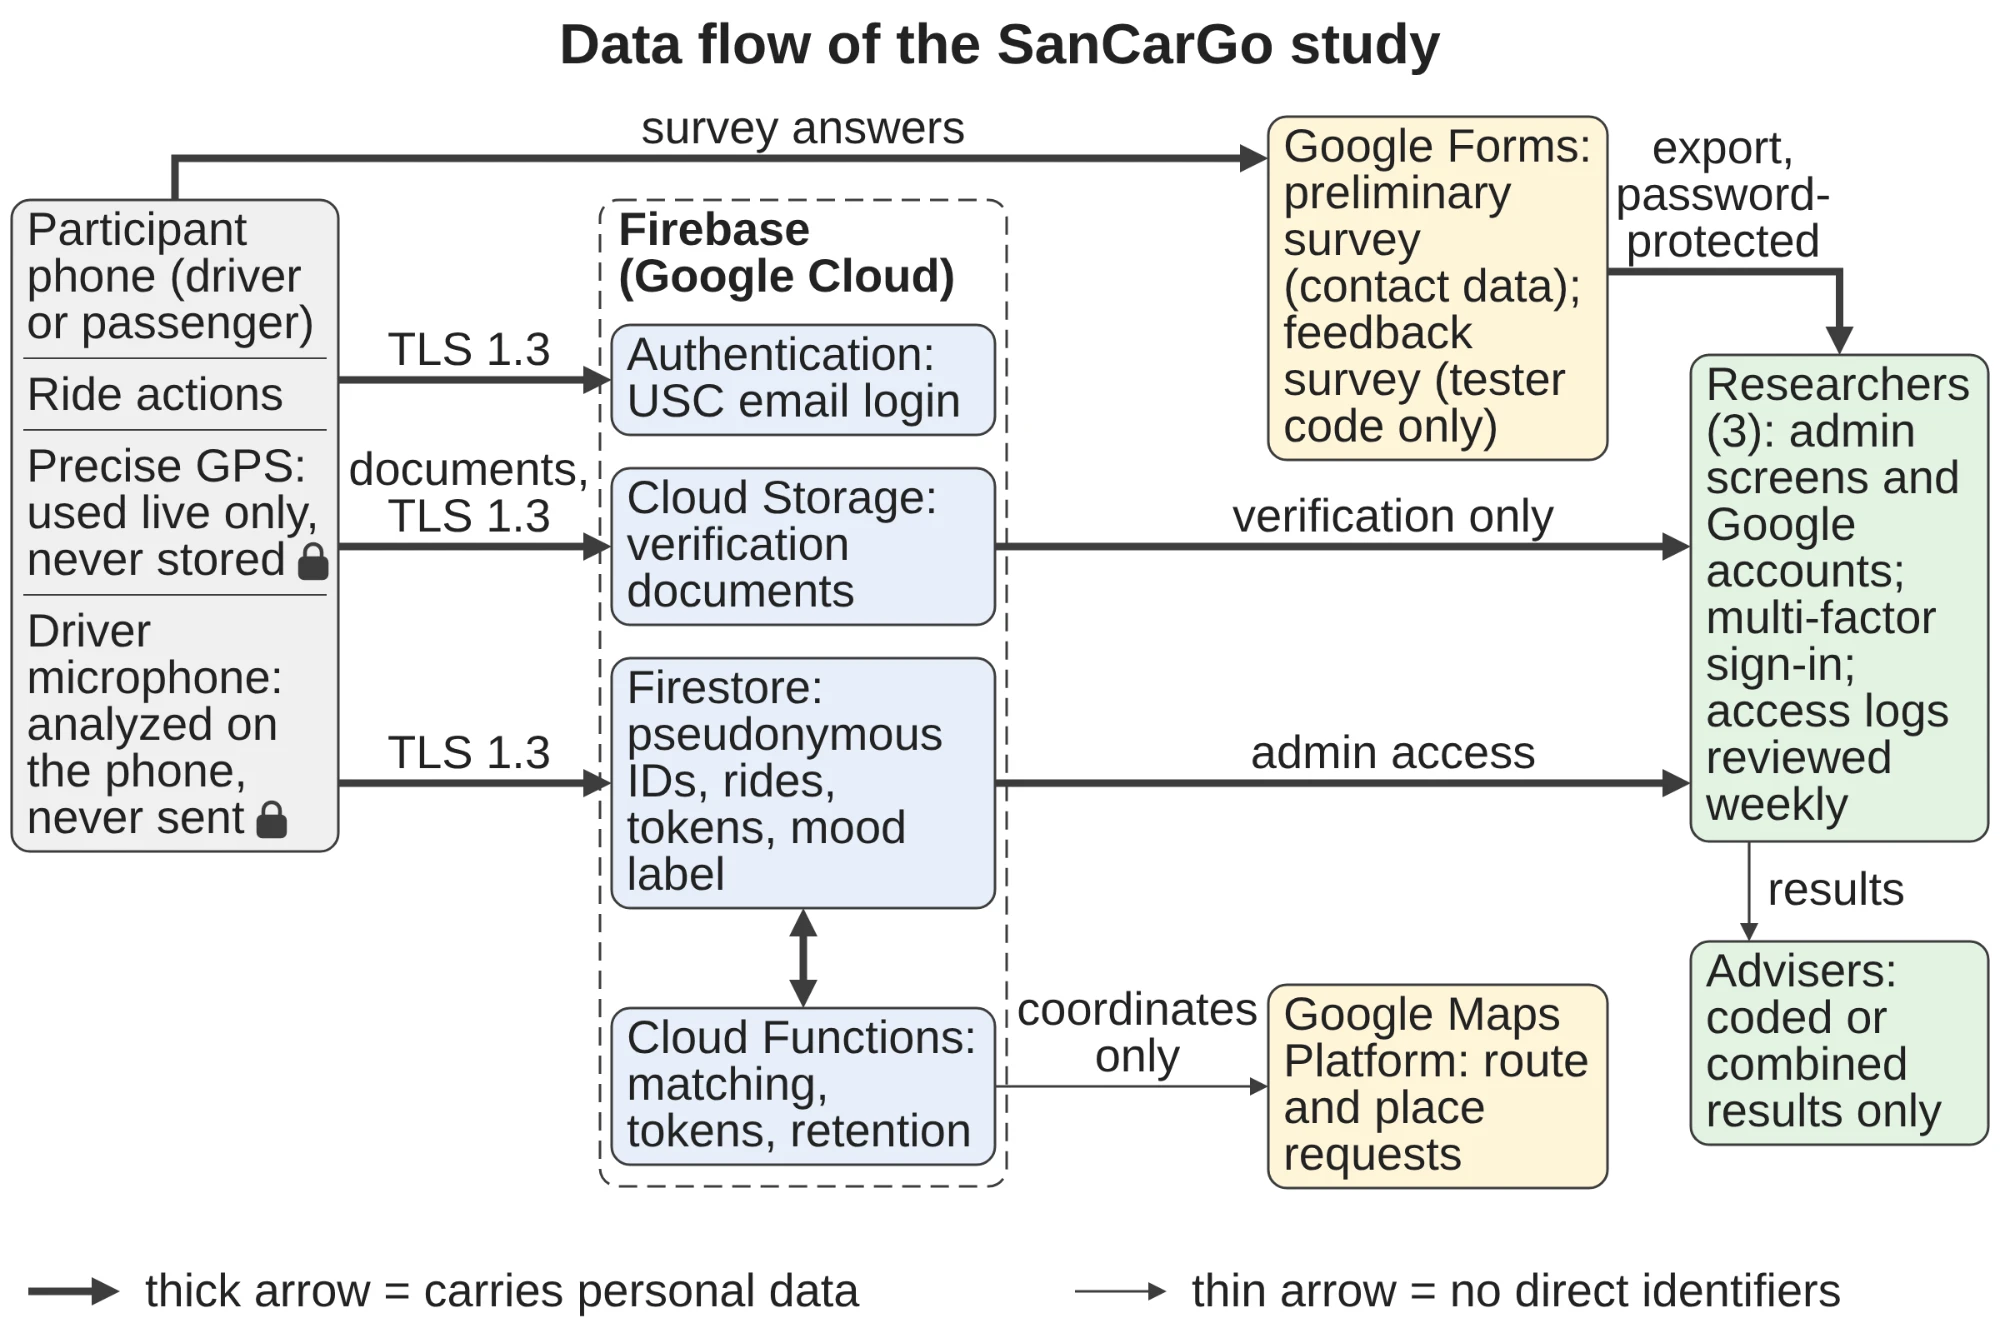
\includegraphics[width=\linewidth]{images/dataflow.png}
\caption[Data flow of the SanCarGo study]{Data flow of the SanCarGo study}\label{fig:dataflow}
\end{figure}

\textit{Storage.} Digital research data are stored in Firebase (Google Cloud) and in the researchers' Google accounts, and downloaded files are kept only in a closed, password-protected folder on the researchers' laptops, which are locked with a password and are not shared. No identifiable research data are kept on removable media such as memory sticks. Backups are made only inside the same accounts. Credentials and encryption keys are kept out of the source code and are restricted to the researchers. Local copies in the phones of the participants (the application cache) are cleared at the end of the testing. Signed paper forms are scanned and kept in a closed folder.

\textit{Access.} Table~\ref{tab:access} shows who may access what. Permissions follow the least-privilege principle, administrator accounts are protected by multi-factor sign-in, and the access logs are reviewed as stated above.

\begin{footnotesize}
\begin{longtable}{p{0.22\textwidth}p{0.62\textwidth}}
\caption[Access-control matrix]{Access-control matrix}\label{tab:access}\\
\hline
\textbf{Role} & \textbf{Access} \\ \hline
\endfirsthead
\hline
\textbf{Role} & \textbf{Access} \\ \hline
\endhead
Participant & Own account, own documents, own rides \\ \hline
Researchers (3) & Pseudonymized research data; documents for verification; the key linking codes to names \\ \hline
Advisers & Coded or combined results only; no identifiable records \\ \hline
Administrators (researchers) & Approval of registrations, reports, and logs, through the admin screens \\ \hline
Others & No access \\ \hline
\end{longtable}
\end{footnotesize}

\subsection[Incidental Findings and Safety Incidents]{Incidental Findings and Safety Incidents}\label{sec:incidental}
An incidental finding is information that appears during the testing without being a purpose of the study, such as a report of unsafe driving, harassment, an accident, or an accidental disclosure of sensitive information. The safety monitor assessed it first, and escalated it to the other researchers and the adviser in case of an injury, a threat, harassment, or a legal issue. Each incident was written in an incident log with only the participant code, the date, and a short description, and no unrelated personal information was collected. Participants were told about this in the informed consent form.

\subsection[Retention and Destruction]{Retention and Destruction}\label{sec:retention}
Retention follows one schedule for each category of data (Table~\ref{tab:data}). Detailed ride records, reports, ratings, emergency events, and requests gathered in the application are deleted after twelve (12) months by a scheduled Cloud Function, which first copies the Ride Token records into an anonymous record of the amount, status, and dates. Accounts and uploaded verification documents are kept until the user deletes the account. Consent forms, survey responses (preliminary and feedback), and the incident log are kept for three (3) years after the completion of the study as proof of consent and for the study records, and are then deleted. The combined results are part of the thesis and contain no names. At each deletion date, the responsible researcher deletes the Firebase data, the Google Forms responses, the downloaded files, the local copies, and the backups of that category, and shreds the paper copies; a second researcher checks the deletion and signs a destruction log. When a participant withdraws, his or her data are deleted on request, including the copies above, except for data that were already irreversibly anonymized or combined into results, which can no longer be taken out. This limit is stated in the informed consent form.

\subsection[Changes from the Proposal on the Advice of the REC]{Changes from the Proposal on the Advice of the REC}\label{sec:rec-changes}
The proposal described the system and the study for a wider setting, with pickup and drop-off points along public roads outside the campus. The design of the system did not change: the application, the routing and matching rules, the mood classifier, and the Ride Token scheme are as described in Sections~\ref{sec:conceptual} to~\ref{sec:tokens}, and they can support routes beyond USC-TC. On the advice of the Research Ethics Committee (REC), which recommended that the research be conducted within the USC-TC campus as a controlled setting, the study was adjusted as follows. The changes concern how the system was tested, and each is described where it applies.
\begin{itemize}
    \item \textbf{Setting.} Testing and demonstration were conducted inside the USC-TC campus only, and no ride was made on public roads. The Bunzel geofence classified the direction of a trip, the Bunzel Point was the fixed terminal, and the other pickup and drop-off points were approved campus buildings, such as SAFAD and SAS (Sections~\ref{sec:routing} and~\ref{sec:uat-safety}).
    \item \textbf{Duration.} The user acceptance testing was planned for two weeks and was held for one week, because the review of the REC took longer than expected (Section~\ref{sec:uat-conduct}).
    \item \textbf{Safety.} A safety protocol and a risk assessment for the rides were added (Sections~\ref{sec:uat-safety} and~\ref{sec:risk}).
    \item \textbf{Data.} The categories of personal data, their legal basis, the data flow, the storage and access, and one retention schedule were stated (Sections~\ref{sec:legal} to~\ref{sec:retention}).
    \item \textbf{Participants.} Eligibility and exclusion criteria were added for both roles, and the parent's permit was removed from the required documents because every participant is an adult who gives his or her own consent (Sections~\ref{sec:phases} and~\ref{sec:registration}).
    \item \textbf{Consent and benefits.} The Informed Consent Form was revised to describe the actual rides, the risks, the emergency procedures, the insurance, and the benefits to the participants (Appendix~\ref{app:icf}).
\end{itemize}
The same practice was followed for the mood design, whose changes from the proposal are stated in Section~\ref{sec:ai}.

\section{Testing Plan} 
\subsection{Testing Phases}
\label{sec:phases}
Testing was carried out in four phases. The first two phases were referred to as alpha testing, and were performed by the proponents. The alpha and beta testing and the dry run before the UAT mostly used the distances of the design setting, and the UAT used those of the controlled setting (Table~\ref{tab:rules-by-setting}). Table~\ref{tab:phases} summarizes the phases and the objective each one supports.

\begin{table}[htbp]
    \centering
    \caption{Testing Phases}
    \label{tab:phases}
    \small
    \renewcommand{\arraystretch}{1.2}
    \begin{tabular}{|>{\raggedright\arraybackslash}p{0.17\textwidth}|>{\raggedright\arraybackslash}p{0.48\textwidth}|>{\raggedright\arraybackslash}p{0.17\textwidth}|}
        \hline
        \textbf{Phase} & \textbf{Scope} & \textbf{Objective} \\
        \hline
        1. Unit testing (alpha) & Ride matching, Ride Token system, and API integration & Objectives 2 and 3 \\
        2. System testing (alpha) & The whole app together: two emulators, the admin side, and the live backend & Objective 1 \\
        3. Beta testing & Volunteer testers use the application on physical iOS and Android devices (rides are played on emulators), followed by the feedback survey & Objective 1 \\
        4. User acceptance testing (UAT) & About 48 Computer Engineering students (25\% of the 191 target respondents) use the application for two weeks, inside the campus only, on physical devices (Android through Firebase App Distribution, iOS through Xcode), followed by the feedback survey & Objective 4 \\
        \hline
    \end{tabular}
\end{table}

\paragraph{Reference standard.} The four phases followed the test levels described in ISO/IEC/IEEE 29119 (Section~\ref{sec:standards}): unit testing of individual rules, system testing of the integrated application, and acceptance testing by the intended users, with beta testing by outside volunteers added before the acceptance phase. Following the documentation practice of the standard, each system test case recorded a step, an expected result, and an actual result per device, and the beta tasks were kept as a fixed written task list (Appendix~\ref{app:beta}). The expected results come from the specified rules, such as the acceptance and route-match distances of Table~\ref{tab:rules-by-setting}, and the token scenarios of Section~\ref{sec:tokens}, which corresponded to the requirement-based test design described in Part 4 of the standard. Part 11 of the standard, on AI-based systems, was a pointer for the mood classifier, which was evaluated on held-out data, on mixed audio, on the phones, and in a rating check on car recordings (Chapter~4). The standard served only as a reference framework; the testing was not assessed for conformance with it.

\paragraph{Testing approach.} The tester tasks and the survey were black box testing: the testers did not know the code and judged the application only by the inputs they gave and the outputs they saw \cite{gfgbox}. Beta testing means that a limited group of real users tries the application and gives feedback, and acceptance testing means that end users check that the application meets their requirements in realistic scenarios \cite{gfgacceptance}. The results were kept in two groups. Functional testing checks that the application works according to its specified requirements \cite{gfgfunctional}; it was the task list, where each task was recorded as Pass, Fail, or Could not try. Non-functional testing checks how well the application works rather than what it does \cite{gfgnonfunctional}; here it was the survey questions on speed, notifications, readability, reliability, and privacy and, in the user acceptance testing, the System Usability Scale. These were the testers' perceptions, not measurements, and no phase timed responses under load, so this study does not claim performance or load testing. The user acceptance phase was judged mainly on these usability and perception questions. The automated and rules tests run by the proponents were white box testing, because the tester knew the code, and checks made with partial knowledge of the internals, such as comparing a token award with the formula, were grey box testing \cite{gfgbox}.

\paragraph{Installing the application on testing devices.}\label{sec:install}
Android and iOS builds were installed in different ways. For alpha and beta testing, and for iOS devices in UAT, the application was built directly onto the device. Android builds for UAT were released through Firebase App Distribution instead (Section~\ref{sec:distribution}).

On Android devices during alpha and beta testing, the proponents built the application onto the device from Android Studio. On iOS devices, the application was installed from Xcode in the following steps, which are also listed in Appendix~\ref{app:download}.
\begin{enumerate}
    \item The person installing the build signed in with an Apple ID in Xcode.
    \item A Bundle Identifier was created for that Apple ID in Firebase and set up in the Google Cloud Console. A new Bundle Identifier was made for each Apple ID.
    \item The GoogleService-Info.plist file of the Bundle Identifier was downloaded from Firebase and configured in Xcode.
    \item In Xcode, under Signing \& Capabilities, the Apple ID was selected under Team and the Bundle Identifier was entered.
    \item The iOS device was plugged in, and Developer Mode was enabled on it.
    \item After the device restarted, the application was built onto it.
    \item On the device, the Apple ID was trusted under General, VPN \& Device Management in the Settings application.
    \item The SanCarGo application could then be opened.
\end{enumerate}
For alpha and beta testing, the proponents signed in with their own Apple IDs and used their own Bundle Identifiers. For the iOS devices in UAT, the proponents asked each participant to sign in with his or her Apple ID in Xcode during onboarding, on the proponents' computer, and every step after that was done in the same way. The proponents used free Apple ID accounts, and an application signed with a free Apple ID stops opening after seven days. The proponents therefore reinstalled the application on each iOS device after seven days.

\subsubsection{Phase 1: Unit Testing}
Unit testing was automated and was white box testing. It ran the Flutter static analysis (\texttt{flutter analyze}), the Flutter test suite (\texttt{flutter test}), the Cloud Functions test suite (\texttt{npm run test:functions}), the Firestore and Storage rules tests (\texttt{npm run test:rules}, run in the Firebase emulator), and a set of nine verification scripts. The Flutter tests were grouped into six areas: accounts and registration, ride flow and matching, tokens, fuel, and the CES period, admin, reports, and ratings, mood detection, and shared interface and safety. The scripts checked that the server campus geofence agreed with the client, the \texttt{matchRide} rules (acceptance distance, geofence-side direction, capacity, and vehicle filters), the Ride Token arithmetic against the scenarios in this manuscript, the routes and Places parsers, the ranking of alternative drop-off points, the Firestore and Storage security rules, and the DOE fuel price parser, which could also be run live against the current DOE report. A few parts had no automated test of their own, namely the eleven push notification triggers, the privacy retention functions, the callable functions that create ride requests and calculate Ride Tokens, the emergency report function, and some client services for the trip lifecycle and notification navigation. These were covered by the system test cases instead.

\subsubsection{Phase 2: System Testing}
System testing ran 32 cases that exercised the application as a whole through its screens, with some checks made against the backend. The cases were grouped into six areas, accounts and admin (S-A1 to S-A6), ride flow (S-B1 to S-B8), matching filters (S-C1 to S-C6), tokens and fuel (S-D1 to S-D4), notifications and chat (S-E1 to S-E4), and safety and privacy (S-F1 to S-F4), and they are listed in Appendix~\ref{app:systemcases}. Each case listed a step, an expected result, and the actual result per device, together with who ran it, the date, and any defect found. The cases were executed on an emulator, with an admin account and the live backend, and then repeated on three physical devices (Table~\ref{tab:devices}). On the physical devices each case was run in five rounds, and it passed only when all five rounds succeeded and failed if at least one round failed. In addition, a set of measurements was recorded per device, taking what was observed rather than an estimate: the time from a ride request to the driver prompt, the time from the driver's acceptance to the passenger's screen update (median of 5 runs each), the cold start time (median of 3 runs), the number of crashes and freezes counted from Firebase Crashlytics and the testers' notes, and the size of the debug build. The checks of the mood AI on the phones are reported separately in Section~\ref{sec:ai-phones}.

\paragraph{Limit on iOS notifications.} The iOS devices could not receive push notifications during alpha testing, because the proponents used free Apple IDs and did not have paid Apple Developer accounts (Section~\ref{sec:scope}). The notification cases (S-E1 to S-E4) could therefore be run only on the emulator and on the Android phone, and not on the two iPhones. Chat itself worked on iOS inside the application, but a message was not announced when the application was closed or in the background.

Every problem found was entered in a defect log with the test that found it, what happened, a severity, an owner, and a status (open, fixed, or won't fix). Severity followed four levels: Critical (data loss, a safety or security problem, or a core flow that is impossible), Major (a feature fails with no workaround), Minor (it works but wrongly), and Cosmetic (it only looks wrong). Alpha testing was considered complete when the exit criteria in Table~\ref{tab:exit} were met.

\begin{table}[htbp]
    \centering
    \caption{Alpha Testing Exit Criteria}
    \label{tab:exit}
    \small
    \renewcommand{\arraystretch}{1.2}
    \begin{tabular}{|>{\raggedright\arraybackslash}p{0.42\textwidth}|>{\raggedright\arraybackslash}p{0.46\textwidth}|}
        \hline
        \textbf{Measure} & \textbf{Target} \\
        \hline
        Flutter unit tests passing & 100\% \\
        Cloud Functions and rules checks passing & All nine verification scripts \\
        System test cases passing & 90\% or more of the 32 cases \\
        Open Critical defects & 0 \\
        Open Major defects & 0, or each has a documented workaround \\
        Crashes in the system runs & 0 on the core flow (S-B1 to S-B3) \\
        \hline
    \end{tabular}
\end{table}

Table~\ref{tab:devices} lists the devices used: the Google Pixel 8 Pro emulator in Android Studio, and three physical devices (one Android phone and two iPhones).

\begin{table}[htbp]
    \centering
    \caption{Devices Used in Alpha Testing}
    \label{tab:devices}
    \small
    \renewcommand{\arraystretch}{1.2}
    \begin{tabular}{|>{\raggedright\arraybackslash}p{0.38\textwidth}|>{\raggedright\arraybackslash}p{0.30\textwidth}|>{\raggedright\arraybackslash}p{0.18\textwidth}|}
        \hline
        \textbf{Device} & \textbf{Operating system} & \textbf{Used as} \\
        \hline
        Google Pixel 8 Pro (Android Studio emulator) & Android 16.0 (Baklava), API 36 & Emulator \\
        Samsung Galaxy A06 5G & Android 16.0 (Baklava), API 36 & Android (physical) \\
        iPhone 17 & iOS 26.6.2 & iOS 1 (physical) \\
        iPhone 15 Pro Max & iOS 26.6.1 & iOS 2 (physical) \\
        \hline
    \end{tabular}
\end{table}

\subsubsection{Phase 3: Beta Testing}
Beta testing checked the application's functions with people who were not part of the development team. It was black box and functional testing. It involved volunteer testers from outside the Computer Engineering department (such as family and friends of the proponents), using physical iOS and Android devices (Table~\ref{tab:betadevices}). Participation was voluntary, and the personal data collected were limited to the tester's account details and a tester code on the survey. Beta testing itself did not require approval from the Research Ethics Committee (REC); only the feedback form was submitted to it.

Testers did not drive or ride. The inbound and outbound rides were played on two Android emulators in Android Studio (Medium Phone with Android 16, and Google Pixel 10a with Android 17), one playing the passenger and one the driver, with simulated GPS, because a ride needs a driver and a passenger in different places at the same time. Moving a vehicle means changing the emulator's location, so nobody had to be on or near campus. The proponents supplied the GPS spots: a spot off campus within 100~m of an approved pickup point for the passenger, a spot within 400~m of that pickup point for the driver, and a spot on campus near the Bunzel Lobby for finishing the trip. A song was played near the driver emulator so that the microphone had something to classify. Every other feature was tested physically: each tester had one physical device with SanCarGo installed. Because registration accepts only \texttt{@usc.edu.ph} email addresses, testers without a USC email used dummy USC accounts created for testing only. The proponents gave each tester the credentials of one of these accounts (a dummy email in the USC domain, usc.edu.ph), and the testers signed up themselves with them. The proponents controlled each mailbox so that the verification email could be confirmed, and provided the files to upload for registration. Because only a few iPhones were available, the iOS testers shared devices. The iPhones could not receive push notifications, and a chat message on iOS is seen only inside the application, so the testers tried the notification and chat tasks on the emulators.

Before each session, the proponents checked that the Cloud Functions and the security rules were deployed and matched the code, that at least one approved pickup point and one drop-off point existed, that the administrator fuel price screen showed a synced price (without one, Ride Tokens could not be computed), and that both emulators could log in, show the map, and receive a test notification. Testers were told that moving means changing the emulator's location, that the emergency button only alerts the administrators and does not call anyone, so they should press Cancel rather than Confirm, that a few Settings rows say they will be added in a future phase, and that nothing in the application involves money.

Each tester followed the task list in Appendix~\ref{app:beta} in order, which was planned to take about 45 minutes with no stopwatch. It had 14 required tasks (T1 to T3 for everyone, and W1 to W11 for one ride) and three optional tasks (O1 to O3) on cancellations and the outbound direction. After the tasks, each tester answered one feedback survey (Section~\ref{sec:survey}, Appendix~\ref{app:survey}), recording Pass, Fail, or Could not try for every task and ratings of their experience. The feedback form was submitted to the Research Ethics Committee (REC).

The proponents separately carried out team checks that testers could not see, as white box and grey box testing. They ran the automated checks on the version under test, registered one account for real (uploading documents, verifying the email, and then approving, denying, and suspending it from the admin side), and went through the admin screens (reviewing a report, approving and dismissing a Ride Token claim, adding and deleting a ride point, refreshing the fuel price, and saving a semester period). They confirmed one emergency alert, checking that every approved admin received the notification and that the event appeared in the admin logs. They took one finished trip and compared its token award with the formula, and checked that a client could not create a ride request directly, write the reward ledger, or read the emergency alerts. One run on a real phone by the proponents was optional, to cover real GPS, battery, background tracking, and push notifications.

Emulator-played rides had limits. They did not show how real GPS drifted on a moving vehicle, battery use and heat, or whether live tracking survived the phone being in a pocket. These limits are stated in Chapter~4 together with the results. The pass marks are in Table~\ref{tab:betapass}.

\begin{table}[htbp]
    \centering
    \caption{Pass Marks for Beta Testing}
    \label{tab:betapass}
    \small
    \renewcommand{\arraystretch}{1.2}
    \begin{tabular}{|>{\raggedright\arraybackslash}p{0.5\textwidth}|>{\raggedright\arraybackslash}p{0.38\textwidth}|}
        \hline
        \textbf{Measure} & \textbf{Target} \\
        \hline
        Task results reported as Pass (ignoring Could not try) & 80\% or more \\
        Core tasks (T1, W2, W4, W6, W8) & No crash reported on any of them \\
        Team checks & All done, with no Critical problem left open \\
        \hline
    \end{tabular}
\end{table}

\begin{table}[htbp]
    \centering
    \caption{Physical Devices Used in Beta Testing}
    \label{tab:betadevices}
    \small
    \renewcommand{\arraystretch}{1.2}
    \begin{tabular}{|c|l|l|}
        \hline
        \textbf{No.} & \textbf{Device} & \textbf{Platform} \\
        \hline
        1 & iPhone 17 & iOS \\
        2 & iPhone 16 & iOS \\
        3 & iPhone 15 Pro Max & iOS \\
        4 & iPhone XR & iOS \\
        5 & Samsung Galaxy Note 8 & Android \\
        6 & Samsung Galaxy A06 5G & Android \\
        7 & Samsung Galaxy A04 & Android \\
        8 & Samsung Galaxy S22 Ultra & Android \\
        9 & Redmi 12C & Android \\
        10 & Huawei Nova Y61 & Android \\
        \hline
    \end{tabular}
\end{table}

\paragraph{Pre-UAT dry run.} Towards the end of beta testing, the proponents went over the flow of the application (Section~\ref{sec:flow}) and asked three people they personally reached out to, such as family members, to try it as a dry run ahead of the UAT. The dry run was not framed as a usability evaluation, and it did not go into technical detail.

\subsubsection{Phase 4: User Acceptance Testing}
The user acceptance testing had four parts, in this order: the preliminary survey of all enrolled Computer Engineering students, which also invited the volunteers; the user acceptance test itself; the distribution of the application to the participants; and the feedback survey that they answered after the test.

\paragraph{Preliminary survey (baseline data collection).}\label{sec:prelim}
\indent Before the application was launched for testing, a Google Forms survey was distributed to all enrolled USC Computer Engineering students. It had two purposes: to collect baseline data for the development of the application, and to invite volunteers for the user acceptance test that followed. The students who answered it are called respondents. Answering the survey did not commit a respondent to the test: each respondent chose whether to be a tester. It took about 3 minutes to answer. The full list of questions is in Appendix~\ref{app:prelim}. The form collected the following:

\begin{itemize}
    \item \textbf{Location.} The city where the respondent primarily lived in the first semester of A.Y. 2026--2027 (Cebu City, Mandaue City, Lapu-Lapu City, Talisay City, or another place), and the nearest major landmark to where the respondent started his or her daily commute. The respondents were told not to enter an exact house number or street address. The landmarks helped the proponents choose pick-up and drop-off zones.
    \item \textbf{Devices.} The operating system of the respondent's phone (iOS, Android, or both), the phone model, and the network carriers used for mobile data. These showed which platforms and network conditions the application had to work on.
    \item \textbf{Interest in user acceptance testing.} Whether the respondent wanted to be a pilot tester for two weeks, and the role he or she wanted to take (both driver and passenger, or passenger only). The answer was the respondent's own choice, and declining had no consequence. A note on the form stated that only student-drivers could earn CES points.
    \item \textbf{Vehicle (for respondents who choose the driver role).} Whether the vehicle with the USC Motor Vehicle Pass sticker is a car or a motorcycle. The study is limited to one registered vehicle per student-driver. Car drivers stated the fuel type, since only gasoline-powered and diesel-powered vehicles were accepted, and the Ride Token computation used the fuel price. Motorcycle drivers stated whether they had a spare helmet to lend to a passenger.
\end{itemize}

Respondents who said they were interested received an email with the date and time of the onboarding for the user acceptance test. About 48 of these volunteers, which was 25\% of the 191 target respondents, were then selected to take part.

This survey data helped refine the application's target user base, determine the driver-to-passenger ratio, and choose the pick-up and drop-off zones.

The survey was sent to all enrolled Computer Engineering students ($N = 378$). The target number of responses followed Cochran's formula \cite{cochran1977} with a 95\% confidence level ($z = 1.96$), a 5\% margin of error ($e$), and an assumed proportion $p = 0.5$:
\begin{equation}
    n_0 = \frac{z^2\, p\,(1-p)}{e^2} \approx 384.16, \qquad
    n = \frac{n_0}{1 + \frac{n_0 - 1}{N}} \approx 190.8 \;\Rightarrow\; 191 \text{ responses.}
\end{equation}
Respondents who were not selected did not receive an incentive. The incentives of the selected participants are described below.

\paragraph{User acceptance test.}\label{sec:uat-test}
UAT evaluated the application in real use. From the respondents who chose to be testers, about 48 Computer Engineering students were to take part, with Years 1 to 3 prioritized because they were on campus more days of the week, which made matching and supervision possible; students of any year level could be selected, and the choice had no effect on grades. The number was 25\% of the 191 target respondents, which is about 48 students, and it was not set by a formula. It was the realistic expectation of the proponents for two reasons: the review of the REC takes time to process, which left little time to recruit and to test, and the controlled setting offered only a few routes that the student testers could take, so a larger group would have been difficult to match and to supervise. UAT was planned to last two weeks and was held inside the USC-TC campus only (Section~\ref{sec:routing}), as the REC recommended.

\textit{Why actual rides are needed.} The beta testing in Phase 3 played the rides on emulators, and it could not show how the real GPS position drifts on a moving vehicle, how the battery and heat behave, whether live tracking continues when the phone is in a pocket, how the driver's microphone hears the cabin of a real vehicle, or how real students perceive the application when they actually offer and take a ride. These were the questions of Objective 4, and acceptance testing means that end users check the application in realistic scenarios~\cite{gfgacceptance}. The risks of real rides are real as well (Section~\ref{sec:lit-risks}), and so the UAT followed the emulator tests and the system tests, was limited to two weeks inside the campus, and was covered by the safety protocol and risk assessment of Sections~\ref{sec:uat-safety} and~\ref{sec:risk}.

\textit{Eligibility and exclusion.} Both roles: a student currently enrolled in the BS Computer Engineering program of USC-TC, at least 18 years old, who answered the preliminary survey, chose to be a tester, and gave informed consent, owned an Android or iOS phone, and uploaded a USC ID and study load that an administrator verified. Drivers also needed a valid driver's license, a valid USC campus vehicle sticker (Motor Vehicle Pass), a registered vehicle, and, for motorcycles, proof of a second helmet. Passengers had no vehicle requirement. A student was excluded if he or she was not enrolled in Computer Engineering, was under 18, could not provide the documents, or had withdrawn consent. The eligibility of a driver was checked by an administrator from the documents, and was separate from whether the student was willing to drive. When more eligible volunteers applied than the target of about 48, the participants were to be chosen from the Years 1 to 3 first, and then from the other year levels, so that drivers and passengers could be matched.

\textit{Voluntariness.} Participation was voluntary. No student was disadvantaged academically or institutionally for declining or withdrawing. The adviser and assistant adviser did not teach or advise any prospective participant, did not take part in selecting participants, and did not see the responses with names. All participants were competent adults, so the procedures for vulnerable populations were not applicable.

\textit{Duration.} The UAT was planned to take about 17 days in total: a one-day onboarding and safety briefing, two weeks of use inside the campus, and a feedback survey of about 5 to 10 minutes within 24 to 48 hours after the two weeks. The optional project-checking demonstration (Section~\ref{sec:checking}) could take additional time.

\textit{Incentives and benefits.} Student-driver participants were rewarded with CES points for their rideshare service through the CES project proposal ``SanCarGo User Acceptance Testing: A Student Ridesharing Service for the USC Community'' (CES PPA Control No. CES2026-1SA-050), which the USC Community Extension Services (CES) Office approved on October 26, 2026 (Appendix~\ref{app:ces}). Student-passengers got a free ride to or from the campus buildings used in the testing. The CES points were separate from the course grade. Ride Tokens earned during UAT were not converted to CES points. All UAT participants also joined a raffle (a single prize drawing, with the GCash prize amount announced at onboarding). No fuel allowance or travel reimbursement was given. UAT participants answered the same feedback form as beta testers, but they saw the System Usability Scale instead of the task results (Section~\ref{sec:survey}), and the UAT was judged mainly on its usability and perception questions, which are non-functional. The target for the System Usability Scale average was 68 or higher.

\paragraph{Distribution of the application.}\label{sec:distribution}
Android builds were released to the UAT participants through Firebase App Distribution, a free service of Firebase that delivers pre-release builds to a list of invited testers. The earlier Kapiot project released its alpha build through the same service~\cite{pepito2022}. It was chosen for three reasons. First, the application needs no app store listing or review, so the proponents can release a build as soon as it is ready. Second, only the people the proponents invite can install it, which keeps the pre-release version limited to the UAT participants who gave their consent. Third, the Firebase tools are already part of the project (Section~\ref{sec:tools}), so no new account or service is needed. iOS builds are not released this way; they are installed from Xcode during onboarding (Section~\ref{sec:install}).

The Android release followed five steps, which are shown in Appendix~\ref{app:download}. The proponents uploaded the build under test to Firebase App Distribution with short release notes, and added the email address of each participant as a tester. Only email addresses in the usc.edu.ph domain were invited, so the pre-release version was limited to USC students. The participants were not placed in groups: each one chose the role (driver or passenger) that he or she wanted to test. The service sent each participant an invitation email with a link. The participant opened the link on the phone that ran the application, signed in with his or her USC (usc.edu.ph) Google account, and accepted the invitation. The participant then followed the prompts to download and install the application, which included allowing the installation when the phone asked. Finally, the participant opened the application, registered with a USC email, and waited for the administrator's approval before following the tester tasks. An invitation was valid for 30 days, and a participant whose invitation had expired asked the proponents for a new one. When the proponents released a corrected build during the UAT period, the testers were notified and updated through the same service, so every participant tested the same version.

\paragraph{Feedback survey (Google Forms evaluation).}\label{sec:survey}
\indent After beta testing and after UAT, testers completed the same Google Form, sent to each tester after the tasks. The form showed each group only its own parts: beta testers answered Parts 1, 2, 4, and 5, and UAT participants answered Parts 1, 3, 4, and 5. Beta testers were identified by a tester code given by the proponents, so that no names were needed. The parts are listed in Appendix~\ref{app:survey}:

\begin{enumerate}
    \item \textbf{About the tester}: the tester code (beta testers only) and how often the tester used ridesharing applications (never, sometimes, or often), which both groups answered.
    \item \textbf{Task results (beta testers only)}: Pass or Fail for every task that was done, and Could not try for an optional task that was not done, with a text box asking what the tester saw instead for every Fail.
    \item \textbf{System Usability Scale (SUS), UAT only}: ten statements rated from 1 (strongly disagree) to 5 (strongly agree).
    \item \textbf{Experience (both groups)}: seven statements rated from 1 to 5 on speed, notification timing, error messages, readability of the screens and map, how easy the emergency button was to find, why location and microphone access were requested, and how safely personal information was handled.
    \item \textbf{Open questions (both groups)}: whether the application crashed, froze, or lost the tester's place; the most confusing part; what was liked most; the one change that would improve it most; and whether the tester would use the application to get to or from campus.
\end{enumerate}

The SUS score of each UAT participant was computed by subtracting 1 from the answer for every odd-numbered statement, subtracting the answer from 5 for every even-numbered statement, adding the ten values, and multiplying the sum by 2.5, which gives a score from 0 to 100:
\begin{equation}
    \text{SUS} = 2.5 \left[ \sum_{i \in \{1,3,5,7,9\}} (x_i - 1) + \sum_{i \in \{2,4,6,8,10\}} (5 - x_i) \right]
\end{equation}
where $x_i$ is the answer to statement $i$. The scores were averaged over the UAT participants, and a score of about 68 is the usual benchmark for average usability. The experience ratings of Part 4 were reported as averages and were testers' perceptions, not measurements.

After each survey closed, the proponents read the comments (every Fail comment in the beta survey and the open responses in both surveys), grouped the repeated ones, and gave each real problem a severity (Critical, Major, Minor, or Cosmetic, as defined in Section~\ref{sec:phases}).

\subsection{Test Cases for Key Features} %\\
\indent Each feature underwent specific test scenarios to confirm that it performed as expected. Below is a breakdown of the major features and their corresponding validation methods:
\begin{enumerate}
    \item Authentication and Sign-Up
        \begin{itemize}
            \item Test Scenario: A user registered using their USC email.
            \item Expected Outcome: 
            A verification link was sent to the email address, and the account could be used only after the link was confirmed and an administrator approved the registration.
            \item Testing Method: Manual testing by attempting sign-ups with valid and invalid credentials.
        \end{itemize}

    \item Ride Request and Matching
        \begin{itemize}
            \item Test Scenario: A passenger requested a ride from their location to USC.
            \item Expected Outcome: The system assigned a nearby available driver, who received a notification to accept or decline the request.
            \item Testing Method: Functional testing using different device combinations (driver and passenger accounts).
        \end{itemize}

    \item Live Tracking and Navigation
        \begin{itemize}
            \item Test Scenario: A passenger tracked their assigned driver in real time.
            \item Expected Outcome: The application continuously updated the driver’s location on the map.
            \item Testing Method: Field testing using two devices in separate locations.
        \end{itemize}
        
    \item Ride Completion and Token System
Test Scenario: Upon completing a ride, the system awarded Ride Tokens to the driver.
Expected Outcome: The correct amount of tokens was credited to the driver’s account.
Testing Method: Simulated rides with pre-defined fare calculations to check accuracy.

    \item CES Point Conversion
        \begin{itemize}
            \item Test Scenario: A user redeemed 100 ride tokens for 1 CES point.
            \item Expected Outcome: The CES point was correctly recorded in the system and appeared in the user’s profile.
            \item Testing Method: Admin verification of CES point logs.
        \end{itemize}
        
    \item Admin Controls
        \begin{itemize}
            \item Test Scenario: An admin suspended a user who had violated the rules.
            \item Expected Outcome: The user’s account was disabled, preventing further ride requests.
            \item Testing Method: Admin attempts to suspend and reinstate test accounts.
        \end{itemize}
\end{enumerate}

\vspace{1em}

\section{Project Checking Strategy}\label{sec:checking}
\indent Following the panelists' instruction, the project checking was a live demonstration of actual ride activity (pickup, driving, and drop-off) with the participants physically present, so the proponents and panelists could observe system behavior, user interaction, and backend updates concurrently. All of it was done inside the USC-TC campus. The participants were drawn from the UAT participants rather than from a separately recruited group. The project checking was held between November 30 and December 4, 2026, in one of the Computer Engineering classrooms or laboratories on the second floor of the Bunzel building, and it followed the safety protocol of Section~\ref{sec:uat-safety}. The pickup and drop-off places of the demonstration were campus buildings: the inbound trip was built around SAS, which was the pickup point of the inbound trip, and the outbound trip started at the Bunzel building and ended at SAFAD and SAS.

\indent The demonstration followed the structured roles below:
\begin{itemize}
    \item Two (2) Student-Drivers proceeded through the registration, logged in to their dashboard menu, and navigated through the app’s driver dashboard.
    \item Four (4) Student-Passengers also registered and logged in through their respective user flow, viewing their version of the dashboard post-verification.
    \item The Proponents managed the approval of all participant registrations using the admin dashboard and monitored backend data changes via Firebase.
\end{itemize}

\vspace{1em}
\indent The simulation was divided into two major trip scenarios:

\subsection[Inbound Trip (iOS -- Driver A)]{Inbound Trip (iOS -- Driver A)}
\vspace{1em}
    \begin{enumerate}
        \item Driver A started at SAFAD, which is outside the Bunzel geofence, and initiated a rideshare trip using an Apple device.
        \item During the trip, Driver A intentionally deviated from the assigned route, using the campus roads only.
        \item The app triggered automatic rerouting through Google Maps.
        \item The AI model activated and rated the sound in the vehicle as ``Lively''.
        \item The system matched Driver A with Passenger A, whose mood preference was also Lively.
        \item Driver A picked up Passenger A at SAS.
        \item Passenger B, who preferred Calm, was not matched with the Lively driver, so the request stayed unmatched. After waiting about two minutes, Passenger B was prompted to change the mood preference and chose Lively (Section~\ref{sec:moodmatch}). Driver A could then see the request and picked up Passenger B at SAS.
        \item The driver completed the trip, arriving at the Bunzel building with both passengers.
    \end{enumerate}

\subsection[Outbound Trip (Android -- Driver B)]{Outbound Trip (Android -- Driver B)}
\vspace{1em}
    \begin{enumerate}
        \item Driver B started at the Bunzel building, inside the geofence, and initiated an outbound rideshare trip using an Android device.
        \item The AI model activated and detected a ``Calm'' mood.
        \item Driver B was matched with Passenger C, who preferred Calm and was waiting in the Bunzel building, and picked Passenger C up there.
        \item The system detected no match with Passenger D, who had no stated preference and whose destination was not aligned with the route of Driver B.
        \item Passenger D was also picked up in the Bunzel building, to test the ride inclusion logic.
        \item Driver B completed the ride by dropping off Passenger C at SAFAD and then Passenger D at SAS.
    \end{enumerate}

\indent This structured testing process ensured all key system components—registration flows, admin controls, routing and rerouting mechanisms, AI-based mood detection, and match compatibility—were executed in observable and verifiable conditions. The test also provided a qualitative basis for evaluating the app’s tolerance for imperfect match cases and real-world variability.


